\documentclass[preprint,12pt]{elsarticle}
\usepackage{mathtools}
\usepackage{subcaption}
\usepackage{booktabs}
\setlength{\marginparwidth}{2cm}
\usepackage{natbib}
\usepackage{changes}
\usepackage{amssymb}
\usepackage{amsmath}
\setlength{\emergencystretch}{2em}

\journal{Electric Power Systems Research}

\begin{document}
\begin{frontmatter}
\title{Nonlinear Observer-Based Control Paradigms for Two-Stage Grid-Connected PV System}

%% use optional labels to link authors explicitly to addresses:
%% \author[label1,label2]{}
%% \affiliation[label1]{organization={},
%%             addressline={},
%%             city={},
%%             postcode={},
%%             state={},
%%             country={}}
%%
%% \affiliation[label2]{organization={},
%%             addressline={},
%%             city={},
%%             postcode={},
%%             state={},
%%             country={}}

\author{Noman Ali, Qudrat Khan, Waqar Alam} %% Author name

%% Author affiliation
\affiliation[Noman Ali, Qudrat Khan]{organization={Department of Electrical Engineering, COMSATS University, Islamabad, Pakistan},
            addressline={qudratullah@comsats.edu.pk}, 
            city={Islamabad},
            postcode={44000}, 
            state={},
            country={Pakistan}}

            \affiliation[Waqar Alam]{organization={Department of Electronics,University of Buner},
            addressline={walam@ubuner.edu.pk}, 
            city={Sowari, Buner},
            postcode={19290}, 
            state={},
            country={Pakistan}}

\begin{abstract}
The global shift toward renewable energy has increased the importance of solar energy as a clean and sustainable power source for various applications. However, it is strongly affected by variations in meteorological conditions, such as solar irradiance and temperature, which directly influence the voltage and current of photovoltaic (PV) arrays. These limitations necessitate the development of effective and robust power control methods for the reliable integration of PV-generated power into utility grids. This study explores the application of nonlinear control strategies to optimize the performance of grid-connected photovoltaic (PV) systems. Two advanced sliding mode control strategies, i.e., the Continuous Twisting Algorithm (CTA) and Discontinuous Integral Control (DIC), are implemented for dual-stage control of the proposed framework. In the first stage, these control schemes effectively track the maximum power point (MPP) under varying solar conditions using a reference voltage obtained through the Perturb and Observe (P\&O) method. By doing so, it outperformed the traditional PI control technique, which is quite slow to adapt to changes in irradiance. In the second stage, the proposed control strategies regulate the inverter efficiency, which is connected to the grid via an inductor-capacitor-inductor (LCL) filter, thereby reducing undesirable harmonics and ensuring high power quality with a unity power factor. In addition, a sliding mode observer is incorporated to estimate critical parameters, i.e., inverter current and capacitor voltage, thus enabling precise control in the dq coordinate system. The simulation results are obtained using the MATLAB/Simulink environment, which validates the superior performance of the proposed control techniques compared with that of the conventional PI control scheme. The proposed control strategy, i.e., CTA, guarantees exceptional stability and consistent reduction in harmonic distortion (THD) during grid power transfer, while the DIC scheme demonstrates minimal error accumulation over time. Stability analysis are carried out against both the control schemes to ensure finite-time convergence and robustness properties.
\end{abstract}

\begin{keyword}
 Grid-connected Systems, Continuous Twisting Algorithm, Discontinuous Integral Control, Total Harmonic Distortion, Observer
\end{keyword}
\end{frontmatter}

\section{Introduction}
\label{sec1}
The global transition to renewable energy sources underscores the critical importance of clean and sustainable power generation systems. Among the various renewable energy technologies, PV systems have emerged as front-runners owing to their ability to offer reliable and environmentally friendly energy solutions. As countries strive to achieve carbon neutrality, PV systems play a pivotal role in reducing greenhouse gas emissions and combating climate change \cite{esram2007comparison}. The increasing demand for green energy is motivated by technological advancements and heightened awareness of the detrimental effects of fossil fuels. Unlike conventional energy sources, solar power generation does not emit harmful pollutants, making it a key contributor to sustainability. This advantage, combined with the environmental benefits, has positioned PV systems as essential components of modern energy systems \cite{saleh2024challenges}.

Recently, the drastic decline in cost of PV panels has made solar energy accessible to a broader population \cite{nikolina2016international,khan2024economics}. The affordability of PV technology is attributed to advancements in manufacturing processes, economies of scale, and increased competition among manufacturers \cite{esram2007comparison}. This development has enabled households, businesses, and utility companies to integrate solar energy solutions into their operations, further driving global adoption. 

PV systems are broadly categorized as either grid-connected or stand-alone systems. A Stand-alone system operates independently and depends on energy storage elements, i.e., battery banks, to ensure a continuous power supply. In contrast, a grid-connected system interacts directly with the utility grid, allowing surplus energy to be fed back into the grid and drawing power when solar energy generation is insufficient. Such configurations eliminate the need for costly energy storage components, making grid-connected systems a reliable and practical solution \cite{carrasco2006power}. Grid-connected PV systems typically consist of two primary architectures: single-stage and two-stage \cite{trujillo2016modeling}. Single-stage systems connect the PV array directly to the grid via a single inverter, hence simplifying the design and reducing costs. However, this approach limits the energy conversion efficiency under different environmental conditions. In contrast, two-stage grid-connected PV systems consist of a DC-DC converter and a DC-AC inverter stage, thus introducing control over Maximum Power Point Tracking (MPPT) and grid synchronization, which enhances adaptability to dynamic operating conditions \cite{kouro2015grid}. This decoupled architecture in two-stage grid-connected PV systems also improves the MPPT performance by ensuring maximum energy harvesting from the PV array under varying irradiance. In addition, the presence of a DC-DC converter enhances voltage regulation, which is critical for the stability of the system. 
%Furthermore, two-stage systems exhibit superior harmonic mitigation capabilities, ensuring compliance with grid codes and reducing power quality issues \cite{prajapati2023comparative}. These benefits make two-stage systems the preferred choice for modern PV installations, particularly for large-scale and high-power applications.
%For instance, a fractional-order (FO) controller based on fractional-order backstepping control (FOBSC) was introduced for a single-phase, two-stage, grid-connected PV system \cite{fahad2020advanced}. The reported simulation results indicate significant improvements in the maximum power extraction, THD reduction, and overall system efficiency compared with those of traditional integer-order controllers.

The main control objectives of two-stage grid-connected PV systems are to maximize power generation, reduce harmonics in the inverter output, and ensure efficient power transfer to the utility grid. In two-stage systems, MPPT is implemented in the DC-DC converter, which improves the efficiency, particularly under varying weather conditions \cite{trujillo2016modeling}. However, harmonics in the inverter output degrade the power quality, hence necessitating the use of filters such as RL, LC, and LCL. Among these, LCL filters offer better attenuation of high-frequency harmonics but require careful design to avoid resonance issues \cite{li2023harmonic}. Additionally, the precise control of the current and voltage in the inverter ensures maximum active power delivery with minimal reactive power \cite{ahmed2022evaluation}. 

To achieve the required features, different MPPT techniques are used to extract the maximum power from PV panels as follows: The incremental conductance method compares incremental and instantaneous conductance for better performance under variant conditions, whereas the perturb and observe (P\&O) method continuously adjusts the voltage to observe changes in power; however, it struggles with rapid fluctuations \cite{soumana2022comparison}. Sliding Mode Control (SMC) strategies, which are known for their robustness in the presence of uncertainties, have been widely explored to enhance the performance of two-stage grid-connected PV systems \cite{liu2022sliding, alnami2024enhanced}. The SMC achieves superior dynamic and steady-state performance compared with traditional P\&O strategies in both off-grid and grid-connected modes, while also demonstrating improved robustness and efficiency, thus outperforming conventional PI controllers in voltage stability and power output. An integral SMC (ISMC)-based control scheme for two-stage three-phase grid-tied PV systems considered MPPT, DC-link voltage regulation, and grid current synchronization and provided accurate MPPT with reduced power oscillations and fast DC-link voltage regulation under varying irradiation conditions \cite{kihal2018robust}. The works in \cite{dash2022photovoltaic,kumar2015sliding} also employed SMC for dual-inverter-based PV systems, resulting in improved energy conversion efficiency and grid compliance. The problem of unbalanced grid voltage with a grid-connected inverter is addressed in \cite{wu2022sliding} using an SMC scheme. The traditional PI controller struggled with second-order harmonic fluctuations and significant grid current distortion, whereas the SMC approach effectively mitigated these issues and enhanced the quality of the current injected into the grid. In summary, numerous researchers have addressed the problem of improved system stability, efficiency, and power quality, i.e., the input-output feedback linearization (IOFL) method \cite{parvathy2020modelling}, backstepping-based techniques \cite{aouadi2018nonlinear,naddami2022nonlinear}, fractional-order backstepping control (FOBSC), adaptive PI and adaptive SMC \cite{zeb2021control}, and the Super Twisting Sliding Mode Controller (ST-SMC) \cite{zeb2020design,dash2024robust}). The results reported in these studies are promising; however, there remains room for the development of a more advanced control structure to address this problem.

This study addresses the control of a two-stage grid-connected PV system by designing two advanced control laws, i.e., the CTA and DIC schemes, to accurately extract maximum power on the DC-DC converter side. The same control structure is employed at the inverter stage to ensure efficient power injection into the grid with high current quality. In the first stage of the design, the Perturb and Observe (P\&O) algorithm generates a reference PV voltage $V_{ref}$. This reference voltage is used to convert the MPPT design problem into an error regulation problem that adapts to changing solar conditions, and the resulting error dynamics are steered to the origin using the proposed CTA and DIC control strategies. In the second stage, a PI control scheme regulates the DC link voltage and determines the reference grid current. To inject power into the utility grid with minimal distortion, the CTA and DIC control schemes are designed in the dq reference frame to ensure high power quality and maintain the total harmonic distortion (THD) within IEEE limits. Because the system states are not always directly available in real-time scenarios, a state estimator is designed to provide the state estimates required for control implementation, which enhances the robustness and performance of the system. The overall system is simulated in the MATLAB/Simulink environment, and a comparative study of the CTA and DIC is conducted. 

The rest of paper is organized as follows. Section 2 presents the overall system configuration of the proposed framework. Section 3 outlines the design procedure for the proposed control strategies. Section 4 describes the design of the MPPT controller. Section 5 introduces the Utkin sliding-mode observer used to estimate the inverter currents and capacitor voltages in the dq-frame. In Section 6, the designs of the CTA and DIC controllers for the grid-side inverter are presented. Section 7 presents the MATLAB/Simulink simulation results under varying irradiance conditions. Section 8 provides a quantitative comparative analysis of the proposed CTA and DIC controllers. Finally, Section 9 concludes the paper and outlines the directions for future work.

\section{Overall System Configuration}
\label{sec2}
To understand the role of each component in the performance and functionality of a two-stage grid-connected PV system, its overall structure must be demonstrated. This section describes the mathematical models of the key components: the PV array, DC-DC converter, DC link, DC-AC inverter, and grid. These models support the design of the proposed reliable control strategies for obtaining maximum power from the PV system, converting energy efficiently, and satisfying utility grid requirements.
\begin{figure}
    \centering
    \includegraphics[width=\linewidth]{two stage control Simple f.png}
    \caption{Block Diagram of overall system}
    \label{fig:system-overview}
\end{figure}
\subsection{The PV Array}
\label{subsec1}
PV arrays consist of individual PV cells connected in series or parallel to convert sunlight into electricity. To understand their performance, a mathematical model is developed as follows
\begin{equation}
I = N_{p}\big(I_{ph} - I_0 ( e^{\frac{\frac{V}{N_{s}}+ I R_s}{n V_t} } - 1) - \frac{\frac{V}{N_{s}} + I R_s}{R_{sh}}\big)
\label{eq:pv_model},
\end{equation}
where \( I \) is the output current, \( V \) is the terminal voltage produced by PV array, \( I_{ph} \) is the photocurrent that depends on irradiance and temperature, \( I_0 \) is the diode saturation current, \( R_s \) is the series resistance, \( R_{sh} \) is the shunt resistance, \( n \) is the ideality factor of the diode, and \( V_t = \frac{k T}{q} \) is the thermal voltage, whereas \( k \) is the Boltzmann constant, \( T \) is the temperature in Kelvin, and \( q \) is the charge of an electron.
\subsection{The Boost Converter}
\label{subsec:boost-converter}
In a two-stage grid-connected PV system, the first stage uses a DC-DC boost converter to adjust the PV voltage so that the array operates at its maximum power point, which maintains system stability and maximizes the energy harvested from the solar panels.
The dynamic model of the DC-DC boost converter in terms of the duty cycle \(D\), inductor current \(i_L\), and PV voltage \(V_{pv}\) can be presented as
\begin{equation}
\frac{d i_L}{dt} = \frac{V_{pv}}{L} - \frac{(1 - D) V_{dc}}{L}
\label{eq:inductor_current}
\end{equation}
\begin{equation}
\frac{d V_{pv}}{dt} = \frac{1}{C_{pv}} \left( I_{pv} - i_L \right),
\label{eq:pv_voltage},
\end{equation}
where \( i_L \) is the inductor current, \( V_{pv} \) is the PV voltage, \( V_{dc} \) is the output voltage, \( I_{pv} \) is the PV array current, \( L \) and \( C_{pv} \) are the inductor and PV-side capacitance, respectively. These equations describe how the PV voltage and inductor current change dynamically with the duty cycle \(D\).
\begin{figure}[t]
\centering
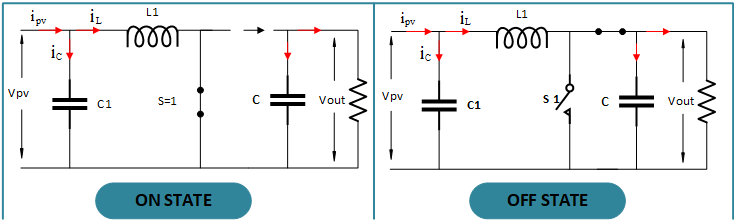
\includegraphics[width = 0.48\textwidth]{BOOST Circuit noman.png}
\caption{Boost converter in (a) ON STATE and (b) OFF STATE}\label{fig1}
\end{figure}
\subsection{Three-Phase Grid-Connected Inverter with LCL Filter}
\label{subsec3}
A three-phase inverter converts DC to AC using six bidirectional switches, each consisting of an Insulated Gate Bipolar Transistor (IGBT) with an antiparallel diode, as shown in Fig.~\ref{fig:grid-inverter}. These switches connect the inverter to the three-phase grid through an LCL filter (\( L_i, C_f, L_g \)). To prevent a DC-link short circuit, the two switches in each leg operate in a complementary manner, i.e., when one is on, the other is off. The inverter has eight possible switching states, two of which produce zero AC line voltage, which allows current to circulate freely. By switching between different states, the inverter generates discrete AC output voltages (\( V_{dc}, -V_{dc} \)), shaping the desired waveform. A modulation strategy ensures valid switching among the states for an efficient operation. Thus, the inverter voltage vector is expressed in terms of the DC link voltage and the switching states.
\begin{figure}
    \centering
    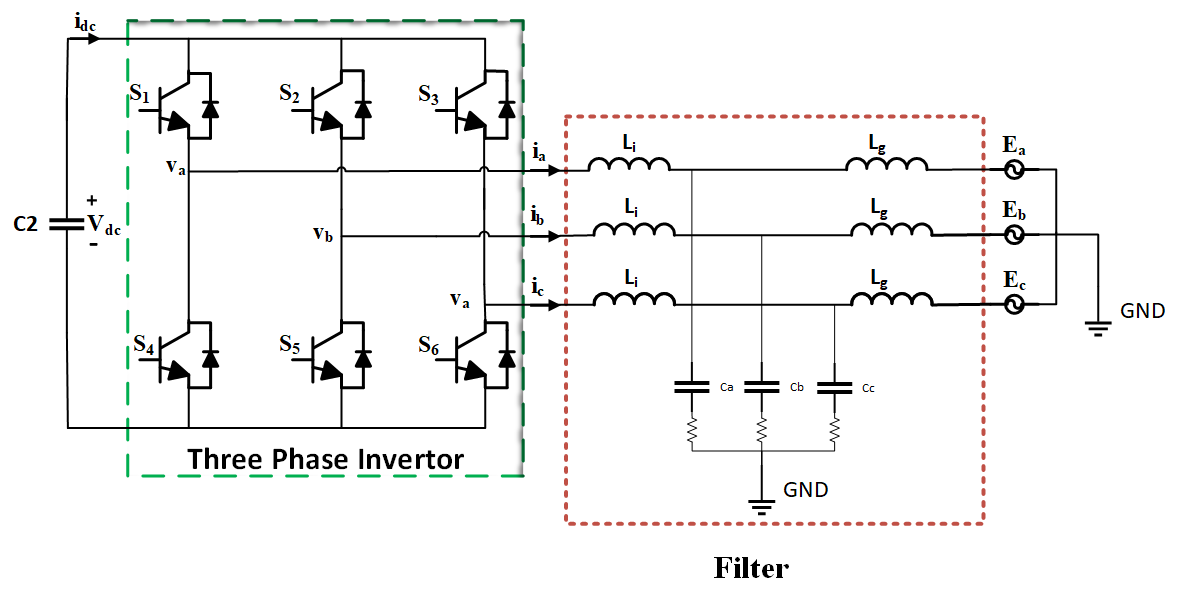
\includegraphics[width=\linewidth]{Grid connected Inverter.png}
    \caption{Schematic diagram of the grid connected three phase inverter with LCL filter}
    \label{fig:grid-inverter}
\end{figure}
As shown in Fig.~\ref{fig:grid-inverter}, the three-phase dynamic model of a grid-connected inverter with an LCL filter in the stationary abc coordinates system is computed using Kirchhoff's laws of voltage and current. The dynamic equations are as follows

\begin{equation}
\left.
\begin{aligned}
\frac{d}{dt}(i_{g_{abc}})=\frac{1}{L_g}v_{c_{abc}}-\frac{1}{L_g}v_{g_{abc}}\\
\frac{d}{dt}(v_{c_{abc}})=\frac{1}{C_f}i_{i_{abc}}-\frac{1}{C}i_{g_{abc}}\\
\frac{d}{dt}(i_{i_{abc}})=\frac{1}{L_i}v_{i_{abc}}-\frac{1}{C_f}v_{c_{abc}}
\end{aligned}
\right\}
\end{equation}

By transforming the system from the abc coordinate system to the dq frame, the number of equations in the system is reduced, and it is easier to use for the control-law design. Transforming Equation (4) into the dq model yields
\begin{equation}
%\sum:
\left\{
\begin{aligned}
    \frac{d}{dt} I_{gd} &= \frac{1}{L_g} V_{cd} + \omega I_{gq} - \frac{1}{L_g} V_{gd} \\
    \frac{d}{dt} V_{cd} &= \frac{1}{C_f} I_d - \frac{1}{C_f} I_{gd} + \omega V_{cq} \\
    \frac{d}{dt} I_d &= -\frac{1}{L_i} V_{cd} + \omega I_q + \frac{1}{L_i} V_d \\
    \frac{d}{dt} I_{gq} &= \frac{1}{L_g} V_{cq} + \omega I_{gd} - \frac{1}{L_g} V_{sgq}\\
    \frac{d}{dt} V_{cq} &= \frac{1}{C_2} I_q - \frac{1}{C_2} I_{gq} - \omega V_{cd} \\
    \frac{d}{dt} I_q &= -\frac{1}{L_i} V_{cq} - \omega I_d + \frac{1}{L_i} V_q
\end{aligned}
\right.
\end{equation}
The state-space representation is crucial for the modeling and control of grid-connected PV systems, as it provides a structured way to analyze the dynamics, design observers i.e., the Utkin observer, and implement an efficient control system. Therefore, the overall state space model of the understudy system can be expressed as

\begin{equation}
%\sum:
\left\{
\begin{aligned}
    \dot{x}_1 &= \frac{1}{L_g} x_2 + \omega x_4 - \frac{1}{L_g} V_{gd} \\
    \dot{x}_2 &= \frac{1}{C_f} x_3 - \frac{1}{C_f} x_1 + \omega x_5 \\
    \dot{x}_3 &= -\frac{1}{L_i} x_2 + \omega x_6 + \frac{1}{L_i} V_d \\
    \dot{x}_4 &= \frac{1}{L_g} x_5 + \omega x_1 - \frac{1}{L_g} V_{gq}\\
    \dot{x}_5 &= \frac{1}{C_2} x_6 - \frac{1}{C_2} x_4 - \omega x_2 \\
    \dot{x}_6 &= -\frac{1}{L_i} x_5 - \omega x_3 + \frac{1}{L_i} V_q
\end{aligned}
\right.
\end{equation}
where \(x_1\), \(x_2\) \(x_3\), \(x_4\), \(x_5\) \(x_6\) correspond to \(I_{gd}\),  \(V_{cd}\), \(I_d\), \(I_{gq}\), \(V_{cq}\) \(I_q\) respectively. The first three dynamics represent d components whereas the later represent q components of the dq coordinate system. Based on the aforementioned dynamics, the control design is presented is follow

\section{Proposed Control Schemes}
\label{sec3}
In this section, the problems associated with the two-stage grid-connected PV system, i.e., maximum power point tracking (MPPT) and  accurate control of inverter to improve power quality, are addressed by designing robust control algorithms, i.e., CTA and DIC-based SMC strategies. In the design of each component, it is prioritized to ensure maximum power extraction from the PV array and to inject it synchronously into the power grid with minimal total harmonic distortion (THD).
\section{Design of MPPT Control}
\label{sec4}
To achieve maximum power point tracking from the photovoltaic array under varying irradiance conditions, the proposed control system is subdivided into two stages, as depicted in the block diagram in Fig.~\ref{fig:mppt-block}. In the first stage, a voltage-based MPPT (V-MPPT) controller is designed using the Perturbation and Observation (P\&O) method to determine a reference voltage \(V_{ref}\). In the second stage, an ISMC-based control law is designed to track the reference voltage \(V_{ref}\) with sufficient accuracy. The boost converter is then controlled by varying the duty cycle \(D\).
\begin{figure}
    \centering
    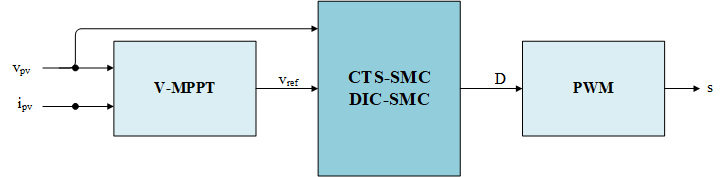
\includegraphics[width=\linewidth]{MPPT.png}
    \caption{Block diagram of proposed VO-MPPT}
    \label{fig:mppt-block}
\end{figure}
\subsection{P\&O-Based V-MPPT}
\label{subsec:po-vmppt}
Based on V-MPPT, a reference voltage \(V_{ref}\) is generated. To this end, the V-MPPT technique is designed to operate using the Perturb and Observe (P\&O) method because of its ease of use and high efficiency, as illustrated in Fig. ~\ref{fig:po-flowchart}. This method systematically varies the voltage and simultaneously measures the resulting change in power, thereby identifying the voltage at which the maximum power is delivered.

\begin{figure}
    \centering
    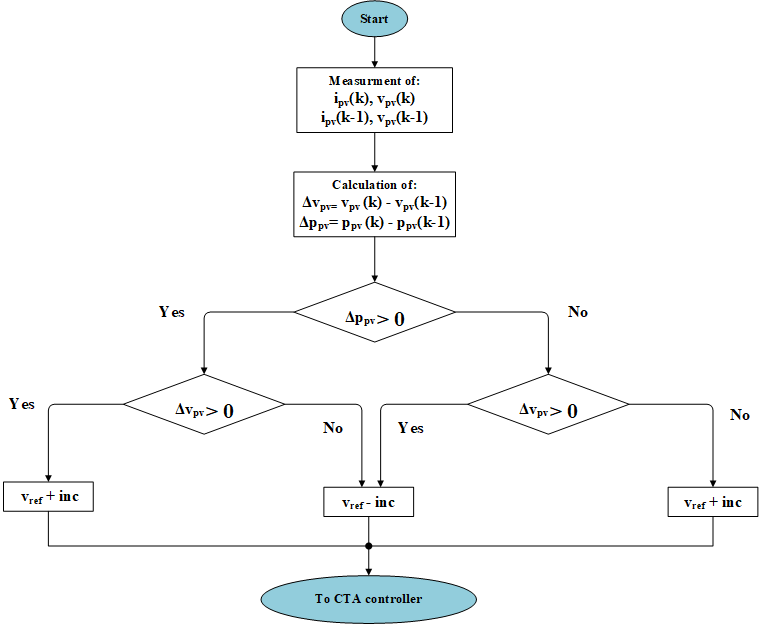
\includegraphics[width=\linewidth]{Flow Chart.png}
    \caption{P\&O based V-MPPT flowchart}
    \label{fig:po-flowchart}
\end{figure}
\subsection{CTA-based Control Design for MPPT}
\label{subsec:cta-mppt}
In the CTA scheme \cite{torres2017design}, the sliding mode control (SMC) mitigates chattering while effectively handling system uncertainties and nonlinearities. Unlike conventional twisting algorithms, the CTA ensures smoother control actions, hence minimizing the mechanical wear in the control loops. Its key advantages include robustness against disturbances, continuous regulation to reduce chattering, and rapid convergence to the sliding manifold. This makes it particularly useful for precision-demanding applications, such as robotics, automotive systems, and aviation. V-MPPT provides a fast response with minimal PV voltage fluctuations under changes in irradiance. Its efficiency relies on the cascade voltage regulator principle. This study proposes an improved V-MPPT-based regulator that accurately determine the duty cycle, ensuring that the boost converter tracks the reference voltage \(V_{ref}\) for optimal PV power extraction. The proposed sliding surface is presented as
\begin{equation}\label{jwdwekjd}
s = \int e_{pv} \, dt,
\end{equation}
where \(e_{pv}\)= \(V_{pv}\) -\(V_{ref}\). 
%Substituting in \label{jwdwekjd} and taking first derivative, we get
%\begin{equation}
%\dot{s} = d ( \int \left( V_{pv} - V_{ref} \right) dt )
%\end{equation}
\begin{equation}\label{dnejde}
\eta' = - \left( k_3 |s|^0 + k_4 |\dot{s}|^0 \right)
\end{equation}
$\eta$ is the structure of the twisting controller \cite{torres2017design}, which is integrated to generate a continuous signal that allows the controller to reject perturbations with bounded derivatives. Substituting the values of \(s\) and \(\dot{s}\) into $\ref{dnejde}$ yields
\begin{equation}
\eta' = - k_3 \left| \int \left( V_{pv} - V_{ref} \right) dt \right|^0 - k_4 \left| V_{pv} - V_{ref} \right|^0 ,
\end{equation}
where \(|s|^a\) = \(|s|^a sign(s)\). The main control law can be written as
\begin{equation}\label{ewjdewkjdbwe}
Duty = -\left( -k_1 |s|^{1/3} - k_2 |\dot{s}|^{1/2} + \eta \right)
\end{equation}
Substituting the values of \(s\) and \(\dot{s}\) into $\ref{ewjdewkjdbwe}$ results in the following control law
\begin{equation}
\begin{aligned}
Duty ={}& -k_1 \left| \int (V_{pv} - V_{ref}) \, dt \right|^{1/3}
          - k_2 |V_{pv} - V_{ref}|^{1/2} \\
        &- k_3 \left| \int (V_{pv} - V_{ref}) \, dt \right|^0
          - k_4 |V_{pv} - V_{ref}|^0 .
\end{aligned}
\end{equation}
\subsection{DIC-based Design for MPPT}
\label{subsec:dic-mppt}
The DIC \cite{moreno2017discontinuous} is a nonlinear control strategy designed to handle dynamic uncertainties and external disturbances, particularly in systems with high variability. Unlike conventional integral controllers, the DIC employs a discontinuous integration approach that enhances the system robustness while preserving stability. It effectively mitigates overshoot and oscillations, making it well-suited for applications requiring precise and rapid control actions, such as Maximum Power Point Tracking (MPPT), Variable Voltage Variable Frequency (VVVF) control, and grid stabilization. Its ability to adapt to disturbances ensures improved inverter performance and power quality regulation in grid-connected systems. By enhancing stability under fluctuating grid conditions, the DIC plays a crucial role in maintaining efficient energy conversion and reliable system operations.
The control law derived for the DIC is as follows
\begin{equation}\label{nwjnww}
    Duty=-k_1 \left| \sigma_1 \right|^{1/3} + \bar{v}
\end{equation}
\begin{equation}\label{fwkfjhw}
    \dot{\bar{v}} = -k_3 \left| \sigma_2 \right|^0,
\end{equation}
where \(\sigma_1\) and \(\sigma_2\) can be presented as
\(\sigma_1=s+k_2 \left|\dot{s} \right|^{3/2}\)
\(\sigma_2=s+k_4 \left|\dot{s} \right|^{3/2}\)

Substituting $\sigma_2$ in $\ref{fwkfjhw}$ and taking its derivatives and then putting it values in $\ref{nwjnww}$ along with $\sigma_1$ results in the overall control law as
\begin{equation}
    Duty = -k_1 \left| s + k_2 \left| \dot{s} \right|^{3/2} \right|^{1/3} - \int \left( k_3 \left| s + k_4 \left| \dot{s} \right|^{3/2} \right|^0 \right) dt
\end{equation}

\section{Design of Utkin Observer}
\label{sec5}
A state observer or state estimator provides internal state observation or estimation by measuring the input and output of a given real system. The system is observed using a computer-implemented program, which serves as the base for many practical systems. However, the implementation of a state observer depends on the complete observability of the system.
Consider the following linear system,
\begin{equation}
    i(t) = Ax(t) + Bu(t) + DU,
\end{equation}
\begin{equation}
    y(t) = Cx(t)
\end{equation}
where \( x(t) \) is the state vector, \( u(t) \) is the input vector, \( y(t) \) is the output vector, \( A \) is the state matrix, \( B \) is the input matrix, \( C \) is the output matrix, \( D \) represents direct feedthrough, and \( U \) is the disturbance vector. The observability of the pair \((A, C)\) for the LCL-filtered grid-connected inverter model considered here is a standard result from the linear systems theory and has been established for similar dq-frame formulations in the literature. Based on this observability property, a Utkin sliding-mode observer can be designed for the proposed system model as follows:

The Utkin observer equation is expressed as follows:

{\scriptsize
\setlength{\arraycolsep}{3pt}
\begin{equation}
\begin{cases}
\dot{\bar{x}}_3 = \left( w\bar{x}_6 + v_{inv\_d} / L_i - \bar{x}_2 / L_i + L_{11}M_1\text{sign}(e_1) + L_{12}M_2\text{sign}(e_2) \right) - G_{11}e_1 - G_{12}e_2 \\

\dot{\bar{x}}_2 = -\left( \bar{x}_1 / C_f - \bar{x}_3 / C_f + L_{21}M_1\text{sign}(e_1) + L_{22}M_2\text{sign}(e_2) \right) - G_{21}e_1 - G_{22}e_2 \\

\dot{\bar{x}}_5 = \left( \bar{x}_6 / C_f - \bar{x}_4 / C_f + L_{31}M_1\text{sign}(e_1) + L_{32}M_2\text{sign}(e_2) \right) - G_{31}e_1 - G_{32}e_2 \\

\dot{\bar{x}}_6 = \left( v_{inv\_q} / L_i - w\bar{x}_3 - \bar{x}_5 / L_i + L_{42}M_2\text{sign}(e_2) + L_{41}M_1\text{sign}(e_1) \right) - G_{41}e_1 - G_{42}e_2 \\

\dot{\bar{x}}_1 = \left( w\bar{x}_4 - v_{gd} / L_g + \bar{x}_2 / L_g - M_1\text{sign}(e_1) - e_1g_{11} - e_2g_{12} \right) \\

\dot{\bar{x}}_4 = \left( \bar{x}_5 / L_g - w\bar{x}_1 - v_{gq} / L_g - M_2\text{sign}(e_2) - e_1g_{21} - e_2g_{22} \right);
\end{cases}
\end{equation}
}
where $\bar{x}$ is the estimated state and $L$ is the observer gain matrix.

\section{Design of Inverter Controllers}
\label{sec:inverter-controllers}
In this section, we present the design of a robust sliding mode control (RSMC) strategy for the inverter stage of a two-stage grid-connected PV system. The proposed control framework integrates the Continuous Twisting Algorithm (CTA) and the Discontinuous Integral Controller (DIC) to ensure maximum power transfer, reduced Total Harmonic Distortion (THD), and precise grid synchronization.

The control design begins with defining the reference grid currents \(i^*_{dg}, i^*_{qg}\), derived from the Maximum Power Point Tracking (MPPT) and DC-link voltage regulation. The CTA-based current controller enforces finite-time convergence, thereby enhancing disturbance rejection and chattering suppression. Simultaneously, the DIC compensates for unknown disturbances, ensuring steady-state accuracy and improved robustness.

To achieve optimal switching control, the computed control signals are fed into a Space Vector Modulation (SVM) scheme, generating the appropriate inverter switching states. The proposed controller effectively stabilizes the system under grid fluctuations and load variations, ensuring compliance with IEEE power quality standards.

\subsection{CTA Controller Design for Inverter}
\label{subsec:cta-inverter}
Initially, the reference direct current \(i^*_{dg}\) is estimated using a PI voltage regulator, as discussed in the preceding section. Concurrently, the reference quadrature current \(i^*_{qg}\) is set to zero, which is a strategic choice designed to prevent the injection of reactive power into the grid, and thereby focus solely on active power transfer. Subsequently, the derived reference voltage vector \(D_d, D_q\) is converted into the abc frame and applied through PWM to control the grid-tied inverter. Additionally, the phase-locked loop (PLL) plays a crucial role in synchronizing the estimated grid phase angle $\theta_g$  with that of the actual grid, which is essential for effectively implementing Park’s transformation. This comprehensive approach ensures a streamlined integration of PV power into the grid, optimizing the stability and efficiency of the power transfer.

\begin{figure}
    \centering
    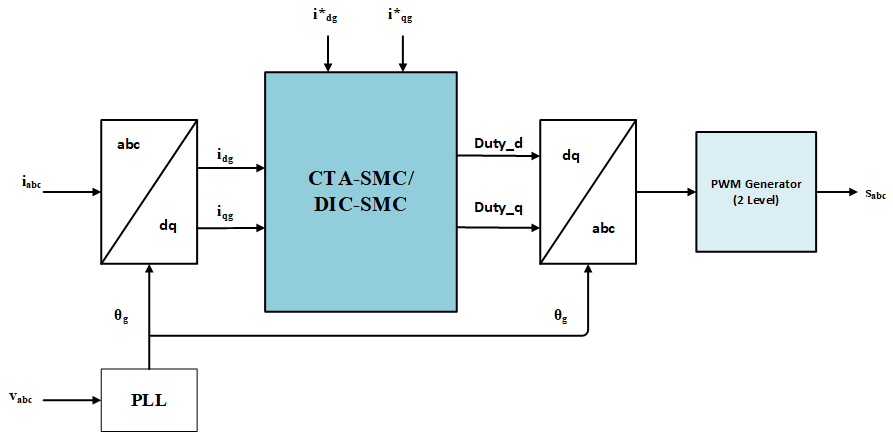
\includegraphics[width=\linewidth]{CTA-SMC Invervter.png}
    \caption{Block diagram of the CTA-SMC-based inverter controller}
    \label{fig:cta-inverter-control}
\end{figure}

\begin{equation}
    e_d = i_{dg}-i^*_{dg}
\end{equation}

\begin{equation}
   e_q = i_{qg}-i^*_{qg}
\end{equation}
where \(e_d\) is the error between currents \(i_{dg}\) and \(i^*_{dg}\) in the d frame, and \(e_q\) is the error between currents \(i_{qg}\) and \(i^*_{qg}\) in the q frame.

Taking derivatives of \(e_d\) and \(e_q\)

\begin{equation}
    e'_d = \frac{di_d}{dt} - \frac{di_{d\_ref}}{dt}
\end{equation}

\begin{equation}
    e'_q =  \frac{di_q}{dt} - \frac{di_{q\_ref}}{dt}
\end{equation}

Where \(\frac{di_d}{dt}\) and \(\frac{di_q}{dt}\) are:

\begin{equation}
    \frac{di_{dg}}{dt} = \frac{V_{cd}}{L_2} + w i_{sgq} - \frac{V_{gd}}{L_2}
\end{equation}

\begin{equation}
    \frac{di_{gq}}{dt} = \frac{V_{cq}}{L_2} - w i_{gd} - \frac{V_{gq}}{L_2}
\end{equation}
Substituting the expressions for \(\frac{di_{dg}}{dt}\) and \(\frac{di_{qg}}{dt}\) into \(e'_d\) and \(e'_q\) yields
\begin{equation}
    e'_d = \frac{V_{cd}}{L_2} + w i_{sgq} - \frac{V_{gd}}{L_2} - \frac{di^*_{dg}}{dt}
\end{equation}

\begin{equation}
    e'_q =  \frac{V_{cq}}{L_2} - w i_{gd} - \frac{V_{gq}}{L_2} - \frac{d^*i_{qg}}{dt}
\end{equation}

where \( V_{cd} \) and \( V_{cq} \) are the filter capacitor voltages in the dq components, and \( V_{gd} \) and \( V_{gq} \) are the grid voltages in the dq components, respectively.

The proposed sliding-mode surfaces are defined in terms of the dq rotating frame as follows:
\begin{equation}
S_d = e_d + Z_d \int e_d dt
\end{equation}

\begin{equation}
S_q = e_q + Z_q \int e_q dt
\end{equation}

where \( Z \) denotes the sliding surface coefficient.

The time derivatives of the equations yield

\begin{equation}
s'_d = e'_d + Z_d e_d
\end{equation}

\begin{equation}
s'_q= e'_q + Z_q e_q
\end{equation}
Substituting the expressions for \( \frac{di_{dg}}{dt} \) and \( \frac{di_{qg}}{dt} \) yields

\begin{equation}
s'_d = \left(\frac{V_{cd}}{L_2} + w i_{sgq} - \frac{V_{gd}}{L_2} - \frac{di^*_{dg}}{dt} + Z_d e_d \right)
\end{equation}

\begin{equation}
s'_q =  \left(
\frac{V_{cq}}{L_2} - w i_{gd} - \frac{V_{gq}}{L_2} - \frac{d^*i_{qg}}{dt} + Z_q e_q
\right)
\end{equation}

The structure of the Twisting Controller \cite{torres2017design} is defined by the parameter \( \eta \), which generates a continuous signal that enables the controller to effectively reject perturbations with bounded derivatives:

\begin{equation}
    \dot{\bar{\eta}}_{d} = -\left( k_3 \lceil s_d \rfloor^0 + k_4 \lceil \dot{s'_d} \rfloor^0 \right).
\end{equation}

\begin{equation}
    \dot{\bar{\eta}}_{q} = -\left( k_3 \lceil s_q \rfloor^0 + k_4 \lceil \dot{s'_q} \rfloor^0 \right).
\end{equation}

Substituting the expressions for \(s_d\) and \(s_q\) into the above equations yields the following:

\begin{equation}
    \dot{\bar{\eta}}_{d} = -\left( k_3 \lceil e_d + Z_d \int e_d dt \rfloor^0 + k_4 \lceil \left(\frac{V_{cd}}{L_2} + w i_{sgq} - \frac{V_{gd}}{L_2} - \frac{di^*_{dg}}{dt} + Z_d e_d \right) \rfloor^0 \right).
\end{equation}

\begin{equation}
    \dot{\bar{\eta}}_{q} = -\left( k_3 \lceil  e_q + Z_q \int e_q dt \rfloor^0 + k_4 \lceil \left(
\frac{V_{cq}}{L_2} - w i_{gd} - \frac{V_{gq}}{L_2} - \frac{d^*i_{qg}}{dt} + Z_q e_q
\right) \rfloor^0 \right).
\end{equation}

where \(\lceil s \rfloor^a = |s|^a {sign}(s)\)

The main control law is given by

\begin{equation}
    D_d = -\left(-k_1 \lceil s_d \rfloor^{1/3} - k_2 \lceil {s'_d} \rfloor^{1/2} + \bar{\eta}_d \right)
\end{equation}
\begin{equation}
    D_d = -\left(-k_1 \lceil s_q \rfloor^{1/3} - k_2 \lceil {s'_q} \rfloor^{1/2} + \bar{\eta}_q \right)
\end{equation}
Substituting the expressions for \(s_d\), \(s'_d\), \(s_q\), and \(s'_q\) into the equations above yields the final overall control law for the inverter in terms of the system parameters.
{\footnotesize
\begin{equation}
\begin{aligned}
    D_d = & -\Bigg(-k_1 \lceil e_d + Z_d \int e_d dt \rfloor^{1/3} 
    - k_2 \Bigg\lceil \left(\frac{V_{cd}}{L_2} + w i_{gq} - \frac{V_{gd}}{L_2} 
    - \frac{di^*_{gd}}{dt} + Z_d e_d \right) \Bigg\rfloor^{1/2} \\
    & -\int\left( k_3 \lceil e_d + Z_d \int e_d dt \rfloor^0 
    + k_4 \Bigg\lceil \left(\frac{V_{cd}}{L_2} + w i_{gq} - \frac{V_{gd}}{L_2} 
    - \frac{di^*_{gd}}{dt} + Z_d e_d \right) \Bigg\rfloor^0 \right) \Bigg).
\end{aligned}
\end{equation}
}

{\small
\begin{equation}
 \begin{aligned}
    D_q = & -\Bigg(-k_1 \lceil e_q + Z \int e_q dt \rfloor^{1/3} 
    - k_2 \Bigg\lceil \left(\frac{V_{cq}}{L_2} - w i_{gq} - \frac{V_{gq}}{L_2} 
    - \frac{di^*_{gq}}{dt} + Z e_q \right) \Bigg\rfloor^{1/2} \\
    & -\int\left( k_3 \lceil e_q + Z \int e_q dt \rfloor^0 
    + k_4 \Bigg\lceil \left(\frac{V_{cq}}{L_2} - w i_{gd} - \frac{V_{gq}}{L_2} 
    - \frac{di^*_{gq}}{dt} + Z e_q \right) \Bigg\rfloor^0 \right) \Bigg).
 \end{aligned}
\end{equation}
}

\subsection{Discontinuous Integral Controller}
\label{subsec:dic-inverter}
The main control law for the discontinuous integral controller is expressed as

\begin{equation}
\left\{
\begin{aligned}
    D_d &= -k_1 \Big\lceil s_d + k_2 \lceil {s'}_d \rfloor^{3/2} \Big\rfloor^{1/3}
    - \int \left( k_3 \Big\lceil s_d + k_4 \lceil {s'}_d \rfloor^{3/2} \Big\rfloor^0 \right) dt \\
    D_q &= -k_1 \Big\lceil s_q + k_2 \lceil {s'}_q \rfloor^{3/2} \Big\rfloor^{1/3}
    - \int \left( k_3 \Big\lceil s_q  + k_4 \lceil {s'}_q \rfloor^{3/2} \Big\rfloor^0 \right) dt
\end{aligned}
\right.
\end{equation}
As derived for the CTA controller, the overall control law for the DIC controller is given below after substituting the values of \(s_d\), \(s'_d\), \(s_q\) and \(s'_q\) in equation(42) and building the dq equations separately.

{\small
\begin{equation}
\begin{aligned}
    D_d &= -k_1 \Bigg\lceil e_d + Z \int e_d dt + k_2 \Big\lceil \frac{V_{cd}}{L_2} + w i_{gq} - \frac{V_{gd}}{L_2} - \frac{di^*_{gd}}{dt} + Z e_d \Big\rfloor^{3/2} \Bigg\rfloor^{1/3} \\
    & \quad - \int \left( k_3 \Bigg\lceil e_d + Z \int e_d dt + k_4 \Big\lceil \frac{V_{cd}}{L_2} + w i_{gq} - \frac{V_{gd}}{L_2} - \frac{di^*_{gd}}{dt} + Z e_d \Big\rfloor^{3/2} \Bigg\rfloor^0 \right)dt \\
\end{aligned}
\end{equation}
}

{\small
\begin{equation}
\begin{aligned}
    D_q &= -k_1 \Big\lceil e_q + Z \int e_q dt  + k_2 \Bigg\lceil \frac{V_{cq}}{L_2} - w i_{gd} - \frac{V_{gq}}{L_2} - \frac{di^*_{gq}}{dt} + Z e_q \Big\rfloor^{3/2} \Bigg\rfloor^{1/3} \\
    & \quad - \int \left( k_3 \Bigg\lceil e_q + Z \int e_q dt + k_4 \Big\lceil \frac{V_{cq}}{L_2} - w i_{gd} - \frac{V_{gq}}{L_2} - \frac{di^*_{gq}}{dt} + Z e_q \Big\rfloor^{3/2} \Bigg\rfloor^0 \right) dt
\end{aligned}
\end{equation}
}

\subsection{Stability Analysis via a Lyapunov Candidate Function}
\label{subsec:stability-discussion}

The preceding subsections established the CTA and DIC control laws for the MPPT and inverter stages. We now analyze their stability explicitly by constructing Lyapunov candidate functions for the closed-loop error dynamics, rather than relying solely on citation of the underlying theorems. The analysis proceeds in three steps for each control loop: (i) the closed-loop error dynamics are cast in a canonical two-state form; (ii) a Lyapunov candidate is proposed and its derivative is evaluated along the closed-loop trajectories to establish convergence; and (iii) the homogeneity of the closed-loop vector field is verified to establish that convergence occurs in \emph{finite time} rather than merely asymptotically. Throughout, we use the notation
\begin{equation}
    \lceil y \rfloor^a := |y|^a\,\mathrm{sign}(y), \qquad \lceil y \rfloor^0 := \mathrm{sign}(y), \qquad a \geq 0,
    \label{eq:power-sign-notation}
\end{equation}
consistent with its use in Sections~\ref{sec4} and \ref{sec:inverter-controllers}.

\paragraph{Standing assumptions.}
\begin{itemize}
    \item[\textbf{(A1)}] The lumped disturbance $\varphi(t,x)$ entering each error channel --- arising from irradiance/temperature variation, PV array nonlinearity, boost-converter parameter uncertainty (MPPT stage), and matched grid/filter disturbances (inverter stage) --- is unknown but bounded with a Lipschitz-continuous, bounded derivative: $|\dot{\varphi}(t,x)| \leq L$ for a known constant $L>0$.
    \item[\textbf{(A2)}] (Matching condition) In the coordinates in which the sliding variable and its derivative are defined, the duty cycle $D$ (respectively $D_d, D_q$) enters the second time-derivative of the sliding variable with a known, bounded-away-from-zero, and constant-sign control-effectiveness gain, which is absorbed into the gains $k_1,\dots,k_4$. This is the standard assumption under which the CTA/DIC design methodologies of \cite{torres2017design,moreno2017discontinuous} apply, and it is consistent with the model reduction implicit in Sections~\ref{sec4} and \ref{sec:inverter-controllers}.
\end{itemize}

\subsubsection{Canonical form of the CTA-controlled MPPT loop}
\label{subsubsec:cta-mppt-canonical}

Let $x_1 := s = \int (V_{pv}-V_{ref})\,dt$ and $x_2 := \dot{s} = e_{pv} = V_{pv}-V_{ref}$, so that trivially
\begin{equation}
    \dot{x}_1 = x_2 .
    \label{eq:mppt-x1-dot}
\end{equation}
Substituting the CTA control law (equation~(13)) and the auxiliary dynamics (equation~(9)) into the plant under Assumption (A2), the closed loop takes the canonical form
\begin{equation}
    \dot{x}_2 = -k_1 \lceil x_1 \rfloor^{1/3} - k_2 \lceil x_2 \rfloor^{1/2} + \eta + \varphi(t,x), \qquad
    \dot{\eta} = -k_3\,\mathrm{sign}(x_1) - k_4\,\mathrm{sign}(x_2).
    \label{eq:mppt-cta-closedloop}
\end{equation}
Introducing the shifted auxiliary state $w := \eta + \varphi(t,x)$, which absorbs the disturbance and vanishes exactly when $\eta$ equals its ideal equivalent-control value $-\varphi$, \eqref{eq:mppt-cta-closedloop} becomes
\begin{equation}
\begin{aligned}
    \dot{x}_1 &= x_2, \\
    \dot{x}_2 &= -k_1 \lceil x_1 \rfloor^{1/3} - k_2 \lceil x_2 \rfloor^{1/2} + w, \\
    \dot{w} &= -k_3\,\mathrm{sign}(x_1) - k_4\,\mathrm{sign}(x_2) + \dot{\varphi}(t,x),
\end{aligned}
    \label{eq:mppt-cta-shifted}
\end{equation}
where, by Assumption (A1), $|\dot\varphi| \leq L$; note that $\varphi$ itself has been cancelled exactly out of the $\dot{x}_2$-equation by the shift, leaving only its bounded derivative as a disturbance acting on the auxiliary state.

\subsubsection{Lyapunov candidate and convergence of the reaching phase}
\label{subsubsec:lyapunov-mppt}

Consider the Lyapunov candidate
\begin{equation}
    V(x_1,x_2) = \frac{3k_1}{4}|x_1|^{4/3} + \frac{1}{2}x_2^2 .
    \label{eq:lyap-mppt}
\end{equation}
$V$ is continuously differentiable, positive definite, radially unbounded, and vanishes only at the origin. Differentiating along the trajectories of \eqref{eq:mppt-cta-shifted},
\begin{equation}
\begin{aligned}
    \dot{V} &= k_1 \lceil x_1 \rfloor^{1/3} \dot{x}_1 + x_2 \dot{x}_2 \\
            &= k_1 \lceil x_1 \rfloor^{1/3} x_2 \\
            & \quad + x_2\left(-k_1 \lceil x_1 \rfloor^{1/3} - k_2 \lceil x_2 \rfloor^{1/2} + w\right) \\
            &= -k_2\,\lceil x_2 \rfloor^{1/2} x_2 + x_2 w \\
            &= -k_2 |x_2|^{3/2} + x_2 w,
\end{aligned}
\label{eq:lyap-mppt-derivative}
\end{equation}
where the two $k_1\lceil x_1\rfloor^{1/3}x_2$ terms cancel exactly, and $\lceil x_2\rfloor^{1/2}x_2 = |x_2|^{3/2}$ because $\mathrm{sign}(x_2)\,x_2=|x_2|$. Hence
\begin{equation}
    \dot{V} \leq -k_2|x_2|^{3/2} + |x_2|\,|w| = -|x_2|\left(k_2|x_2|^{1/2} - |w|\right).
    \label{eq:lyap-mppt-bound}
\end{equation}
Equation~\eqref{eq:lyap-mppt-bound} shows that $\dot V < 0$ whenever $|x_2| > (|w|/k_2)^2$, so that $(x_1,x_2)$ is driven into, and remains ultimately bounded within, a neighborhood of the origin whose radius shrinks as $|w|\to 0$. The auxiliary dynamics $\dot w = -k_3\,\mathrm{sign}(x_1) - k_4\,\mathrm{sign}(x_2) + \dot\varphi$ constitute exactly the discontinuous integral sub-loop analyzed in \cite[Thm. ~1]{torres2017design}: provided $k_3, k_4$ are chosen sufficiently large relative to the disturbance bound $L$ (the precise algebraic condition of that theorem), $w$ is driven to zero in finite time. Cascading this fact through \eqref{eq:lyap-mppt-bound} (a standard nested-Lyapunov argument for higher-order sliding-mode loops) shows that the ultimate bound on $(x_1,x_2)$ shrinks to zero, i.e., $(x_1,x_2)=(s,\dot s) \to (0,0)$.

\subsubsection{Homogeneity and finite-time convergence}
\label{subsubsec:homogeneity}

To confirm that this convergence occurs in \emph{finite} time (rather than merely asymptotically), consider the dilation
\begin{equation}
    \Delta_r(t,x_1,x_2,w) = (rt,\; r^3x_1,\; r^2x_2,\; rw), \qquad r>0.
    \label{eq:dilation}
\end{equation}
Direct substitution into the nominal ($\dot\varphi \equiv 0$) closed loop \eqref{eq:mppt-cta-shifted} verifies that every term scales consistently with the weight vector $(q_1,q_2,q_3)=(3,2,1)$ assigned to $(x_1,x_2,w)$:
\begin{equation}
\begin{aligned}
    \frac{d(r^3x_1)}{d(rt)} &= r^2 x_2, \\
    \frac{d(r^2x_2)}{d(rt)} &= r\left(-k_1\lceil x_1\rfloor^{1/3} - k_2\lceil x_2\rfloor^{1/2}+w\right), \\
    \frac{d(rw)}{d(rt)} &= -k_3\,\mathrm{sign}(x_1) - k_4\,\mathrm{sign}(x_2),
\end{aligned}
\label{eq:homogeneity-check}
\end{equation}
which is precisely the original vector field evaluated at $(x_1,x_2,w)$ multiplied by $r^{q_i+\nu}/r^{q_i}=r^\nu$ with $\nu = -1$ in each of its components. The closed loop \eqref{eq:mppt-cta-shifted} is therefore homogeneous of \emph{negative} degree $\nu=-1$ with respect to the weights $(3,2,1)$. By the homogeneity-based finite-time stability theorem of Bhat and Bernstein (\emph{negative-degree homogeneity together with local asymptotic stability of the origin implies global finite-time stability}), and given that the local asymptotic stability of \eqref{eq:mppt-cta-shifted} is established for suitably chosen gains in \cite[Thm. ~1]{torres2017design}, the origin $(x_1,x_2,w)=(0,0,0)$, equivalently $(s,\dot s)=(0,0)$, is reached in a finite time.

As a consistency check, this homogeneity structure predicts that robustness against a disturbance bound $L$ requires the gains to scale as $k_1 \propto L^{2/3}$, $k_2 \propto L^{1/2}$, $k_3 \propto L$, $k_4 \propto L$ (since $x_1,x_2,w$ carry weights $3,2,1$ and $\lceil x_1\rfloor^{1/3}$, $\lceil x_2\rfloor^{1/2}$ must each carry the same weight, $1$, as $w$). This is precisely the scaling law reported for the implemented gains in Table~\ref{tab:gains} ($K_1 \propto \eta^{0.667}$, $K_2 \propto \eta^{0.5}$, $K_3 \propto \eta$, $K_4 \propto \eta$), providing an independent structural confirmation that the tuned gains are consistent with the finite-time stability conditions derived above.

\subsubsection{Exact maximum-power tracking on the sliding manifold}
\label{subsubsec:exact-mppt-tracking}

A notable feature of the MPPT loop is that $x_2$ \emph{is} the physical tracking error, that is, $x_2 = e_{pv} = V_{pv}-V_{ref}$. Consequently, once $(x_1,x_2)$ reaches the origin at some finite time $T$, the invariance of the origin under \eqref{eq:mppt-cta-shifted} guarantees $x_2(t) \equiv 0$ for all $t \geq T$, i.e.,
\begin{equation}
    V_{pv}(t) = V_{ref}(t), \qquad \forall\, t \geq T,
    \label{eq:exact-mppt}
\end{equation}
Therefore, the PV voltage tracks the P\&O-generated reference \emph{exactly} (not merely asymptotically) once the sliding manifold is reached, confirming the maximum power point tracking objective of Section~\ref{sec4}.

\subsubsection{Stability of the DIC-controlled MPPT loop}
\label{subsubsec:dic-mppt-stability}

For the DIC controller (equations~(15)--(19)), recall the two auxiliary sliding variables
\begin{equation}
    \sigma_1 = x_1 + k_2\lceil x_2\rfloor^{3/2}, \qquad \sigma_2 = x_1 + k_4\lceil x_2\rfloor^{3/2}, \qquad k_2 \neq k_4,
    \label{eq:sigma-dic}
\end{equation}
with the control law $D = -k_1\lceil\sigma_1\rfloor^{1/3}+\bar v$, $\dot{\bar v}=-k_3\,\mathrm{sign}(\sigma_2)$. Two observations establish the stability. First, a direct structural argument: if $\sigma_1=\sigma_2=0$ simultaneously, then subtracting the two definitions gives $(k_2-k_4)\lceil x_2\rfloor^{3/2}=0$; because the tuned gains satisfy $k_2\neq k_4$ (Table~\ref{tab:gains} uses $k_2=0.05$, $k_4=4.5$ for the MPPT-DIC loop), this forces $x_2=0$, and then $\sigma_1=0$ forces $x_1=0$. Hence, the \emph{simultaneous} vanishing of the two auxiliary variables is equivalent to $(x_1,x_2)=(s,\dot s)=(0,0)$, exactly as required. Second, by the discontinuous-integral-control theorem of \cite{moreno2017discontinuous}, under Assumption (A1) and gains $k_1,k_2,k_3,k_4>0$ satisfying the algebraic conditions of that reference (matched in Table~\ref{tab:gains} by the relation $K_3 = \eta/l$, which ties the integral gain directly to the disturbance-bound parameter $\eta$, exactly as required by the cited theorem), $\sigma_1$ and $\sigma_2$ are driven to zero in finite time, and therefore so is $e_{pv}=x_2$, by the same argument as in \eqref{eq:exact-mppt}.

\subsubsection{Extension to the inverter current-tracking loops}
\label{subsubsec:inverter-stability}

The dq-frame current loops share the same mathematical structure as the MPPT loop, with two simplifications that are worth noting. First, the cross-coupling terms $\omega i_{gq}$ and $\omega i_{gd}$ that appear in the open-loop dynamics (equations for $\dot i_{dg}, \dot i_{gq}$) are fed forward and cancelled explicitly inside the control laws $D_d, D_q$ (equations~(38)--(41)), so that the closed-loop $d$- and $q$-axis error dynamics decouple into two independent scalar problems, each of the canonical form \eqref{eq:mppt-cta-shifted}. Second, unlike the MPPT loop, the inverter sliding variables are proportional-integral combinations,
\begin{equation}
\begin{aligned}
    S_d &= e_d + Z_d\!\int e_d\,dt, \qquad & S_q &= e_q + Z_q\!\int e_q\,dt, \\
    e_d &= i_{dg}-i^*_{dg}, \qquad & e_q &= i_{qg}-i^*_{qg},
\end{aligned}
    \label{eq:sd-sq-recall}
\end{equation}
Therefore, by setting $y_1:=S_d$, $y_2:=\dot S_d = e'_d+Z_de_d$ (and analogously for the $q$-axis), the pair $(y_1,y_2)$ satisfies $\dot y_1 = y_2$ exactly, and under Assumption (A2), the CTA law of equation~(37) [or the DIC law of equation~(42)] closes the loop on $(y_1,y_2)$ in precisely the canonical form \eqref{eq:mppt-cta-shifted}. The Lyapunov candidate
\begin{equation}
    V_{\text{inv}} = \frac{3k_1}{4}\left(|S_d|^{4/3}+|S_q|^{4/3}\right) + \frac{1}{2}\left(\dot S_d^2 + \dot S_q^2\right)
    \label{eq:lyap-inverter}
\end{equation}
is the sum of two independent copies of \eqref{eq:lyap-mppt}, and by \eqref{eq:lyap-mppt-derivative}--\eqref{eq:lyap-mppt-bound} applied axis-by-axis,
\begin{equation}
    \dot V_{\text{inv}} \leq -k_2\left(|\dot S_d|^{3/2}+|\dot S_q|^{3/2}\right) + |\dot S_d|\,|w_d| + |\dot S_q|\,|w_q|,
    \label{eq:lyap-inverter-derivative}
\end{equation}
Therefore, by the same homogeneity and cascading arguments of Sections~\ref{subsubsec:lyapunov-mppt}--\ref{subsubsec:homogeneity}, both $(S_d,\dot S_d)$ and $(S_q,\dot S_q)$ are driven to the origin in finite time under the CTA law, and the analogous argument of Section~\ref{subsubsec:dic-mppt-stability} applies verbatim (with $x_1\to S_d,\,x_2\to \dot S_d$, respectively $S_q,\dot S_q$) to the DIC law of equation~(42).

\subsubsection{Exponential convergence of the current-tracking error}
\label{subsubsec:exp-convergence-current}

Unlike the MPPT loop, $y_2=\dot S_d$ is \emph{not} the physical tracking error $e_d$, so reaching $(S_d,\dot S_d)=(0,0)$ at a finite time $T_d$ does not make $e_d$ vanish instantaneously. Instead, the invariance of the sliding manifold under the CTA/DIC laws guarantees $S_d(t)\equiv 0$ for all $t \geq T_d$, so that differentiating $S_d\equiv 0$ gives the exact linear error dynamics
\begin{equation}
    \dot e_d(t) = -Z_d\,e_d(t), \qquad t \geq T_d,
    \label{eq:ed-reduced}
\end{equation}
whose solution, using the Lyapunov function $V_{e_d}=\tfrac{1}{2}e_d^2$ with $\dot V_{e_d} = e_d\dot e_d = -Z_de_d^2 = -2Z_dV_{e_d}$, is
\begin{equation}
    e_d(t) = e_d(T_d)\,e^{-Z_d(t-T_d)} \longrightarrow 0 \quad \text{exponentially, provided } Z_d>0,
    \label{eq:ed-exponential}
\end{equation}
and identically for $e_q(t) = e_q(T_q)e^{-Z_q(t-T_q)}$ with $Z_q>0$. Thus, the grid current-tracking loop exhibits \emph{finite-time reaching} of the sliding manifold, followed by \emph{exponential} convergence of the tracking error to zero, in contrast to the MPPT loop, where the tracking error itself vanishes exactly at the finite reaching time (Section~\ref{subsubsec:exact-mppt-tracking}). Because $Z_d, Z_q > 0$ were selected as design parameters in Section~\ref{subsec:cta-inverter}, this condition is satisfied by construction.

\subsubsection{Overall closed-loop stability}
\label{subsubsec:overall-stability}

Collecting the results above: (i) the MPPT loop drives $V_{pv}$ to $V_{ref}$ exactly in a finite time under both the CTA and DIC designs; (ii) the resulting accurate DC-link voltage reference is regulated by the outer PI loop, whose linear dynamics are exponentially stable by standard design; and (iii) the inner dq-frame current loop drives the current-tracking errors $e_d, e_q$ to zero exponentially, following finite-time reaching of the sliding manifold under both the CTA and DIC designs. Because the MPPT, DC link, and current loops operate on well-separated time scales (the current loop is the fastest, consistent with the gain magnitudes in Table~\ref{tab:gains}), the standard cascade/singular-perturbation argument for multi-loop sliding-mode systems applies, and the interconnection of the three loops is locally asymptotically stable, with the sliding-mode subsystems converging in finite time, as established above. This is consistent with the transient behavior observed in the simulations in Section~\ref{sec:results}.

\section{Simulation Results and Discussion}
\label{sec:results}
The controllers designed in Sections~\ref{sec4}--\ref{sec:inverter-controllers} were implemented on the system shown in Fig. ~\ref{fig:system-overview} and evaluated under varying irradiance and temperature. The performance of the system was analyzed using multiple metrics, including MPPT tracking, DC link voltage regulation, output current and voltage, and active/reactive power control. A comparative study was conducted between the proposed controllers (CTA-SMC for both MPPT and inverter) and a conventional PI controller to highlight their effectiveness. The control strategies derived in the previous sections are based on finite-time sliding mode methodologies, ensuring robust and precise control enforcement. This section presents the simulation results of the proposed controllers alongside the PI controller, followed by a detailed analysis.

Numerical simulations were performed using MATLAB/Simulink to compare the proposed method with the conventional approach. The key specifications are summarized in Table\ref{tab:system-params}. The DC link reference voltage was set to 750 V, and the reference current \(i^*_{gq}\) was maintained at zero to ensure only active power injection. It is well established that while temperature has a negligible impact on the PV array's Maximum Power Point (MPP), irradiance plays a critical role in its performance. Therefore, the proposed control technique was tested under varying irradiance conditions, as shown in Fig. ~\ref{fig:irradiance-profile}, with the temperature maintained constant at 25°C. To ensure a fair comparison, identical conditions and parameters were applied to both the proposed and PI-based control methods.
\begin{table}[htbp]
    \centering
    \caption{System Parameters}
    \label{tab:system-params}
    \begin{tabular}{p{6cm} p{4cm}}
        \toprule
        \textbf{Parameters} & \textbf{Value} \\
        \midrule
        Typical peak power & 213 W \\
        Voltage at peak power & 29 V \\
        Current at peak power & 7.35 A \\
        Short-circuit current & 7.84 A \\
        Open-circuit voltage & 36.3 V \\
        Temperature coefficient of $I_{sc}$ & 0.102 (\%/$^{\circ}$C) \\
        Temperature coefficient of $V_{oc}$ & -0.361 (\%/$^{\circ}$C) \\
        Grid voltage & 380 V \\
        Grid frequency ($f$) & 50 Hz \\
        Grid inductance ($L$) & $10^6$ \\
        \bottomrule
    \end{tabular}
\end{table}
The LCL filter parameters are listed in Table~\ref{tab:lcl-params}.
\begin{table}[htbp]
    \centering
    \caption{LCL Filter Parameters}
    \label{tab:lcl-params}
    \begin{tabular}{p{6cm} p{4cm}}
        \toprule
        \textbf{Parameters} & \textbf{Value} \\
        \midrule
        Filter Inductance (L1) & $9.1 \times 10^{-4}$ mH \\
        Filter Capacitance ($C_f$) & 0.5 mF \\
        Filter Inductance (L2) & 5.5 mH \\
        Damping Resistance & 0.3 $\Omega$ \\
        \bottomrule
    \end{tabular}
\end{table}
\subsection{Irradiance and Power}
The system uses solar irradiance as a key input to determine its output power. Fig.~\ref{fig:irradiance-profile} illustrates the variation in solar irradiance over an 8-hour period, representing a typical sunny day in Islamabad, Pakistan. Irradiance peaked during midday and gradually decreased until sunset. Islamabad receives an average of 6–7 h of sunshine daily, with annual sunshine hours ranging between 3,000 and 3,300 h. These fluctuations in irradiance directly affect the electric current and power output of PV systems. Specifically, higher irradiance levels lead to increased current flow and power generation, whereas lower irradiance levels result in a reduced output. This relationship underscores the importance of robust control strategies for maintaining optimal performance under varying irradiance.
\begin{figure}[htbp]
\begin{center}
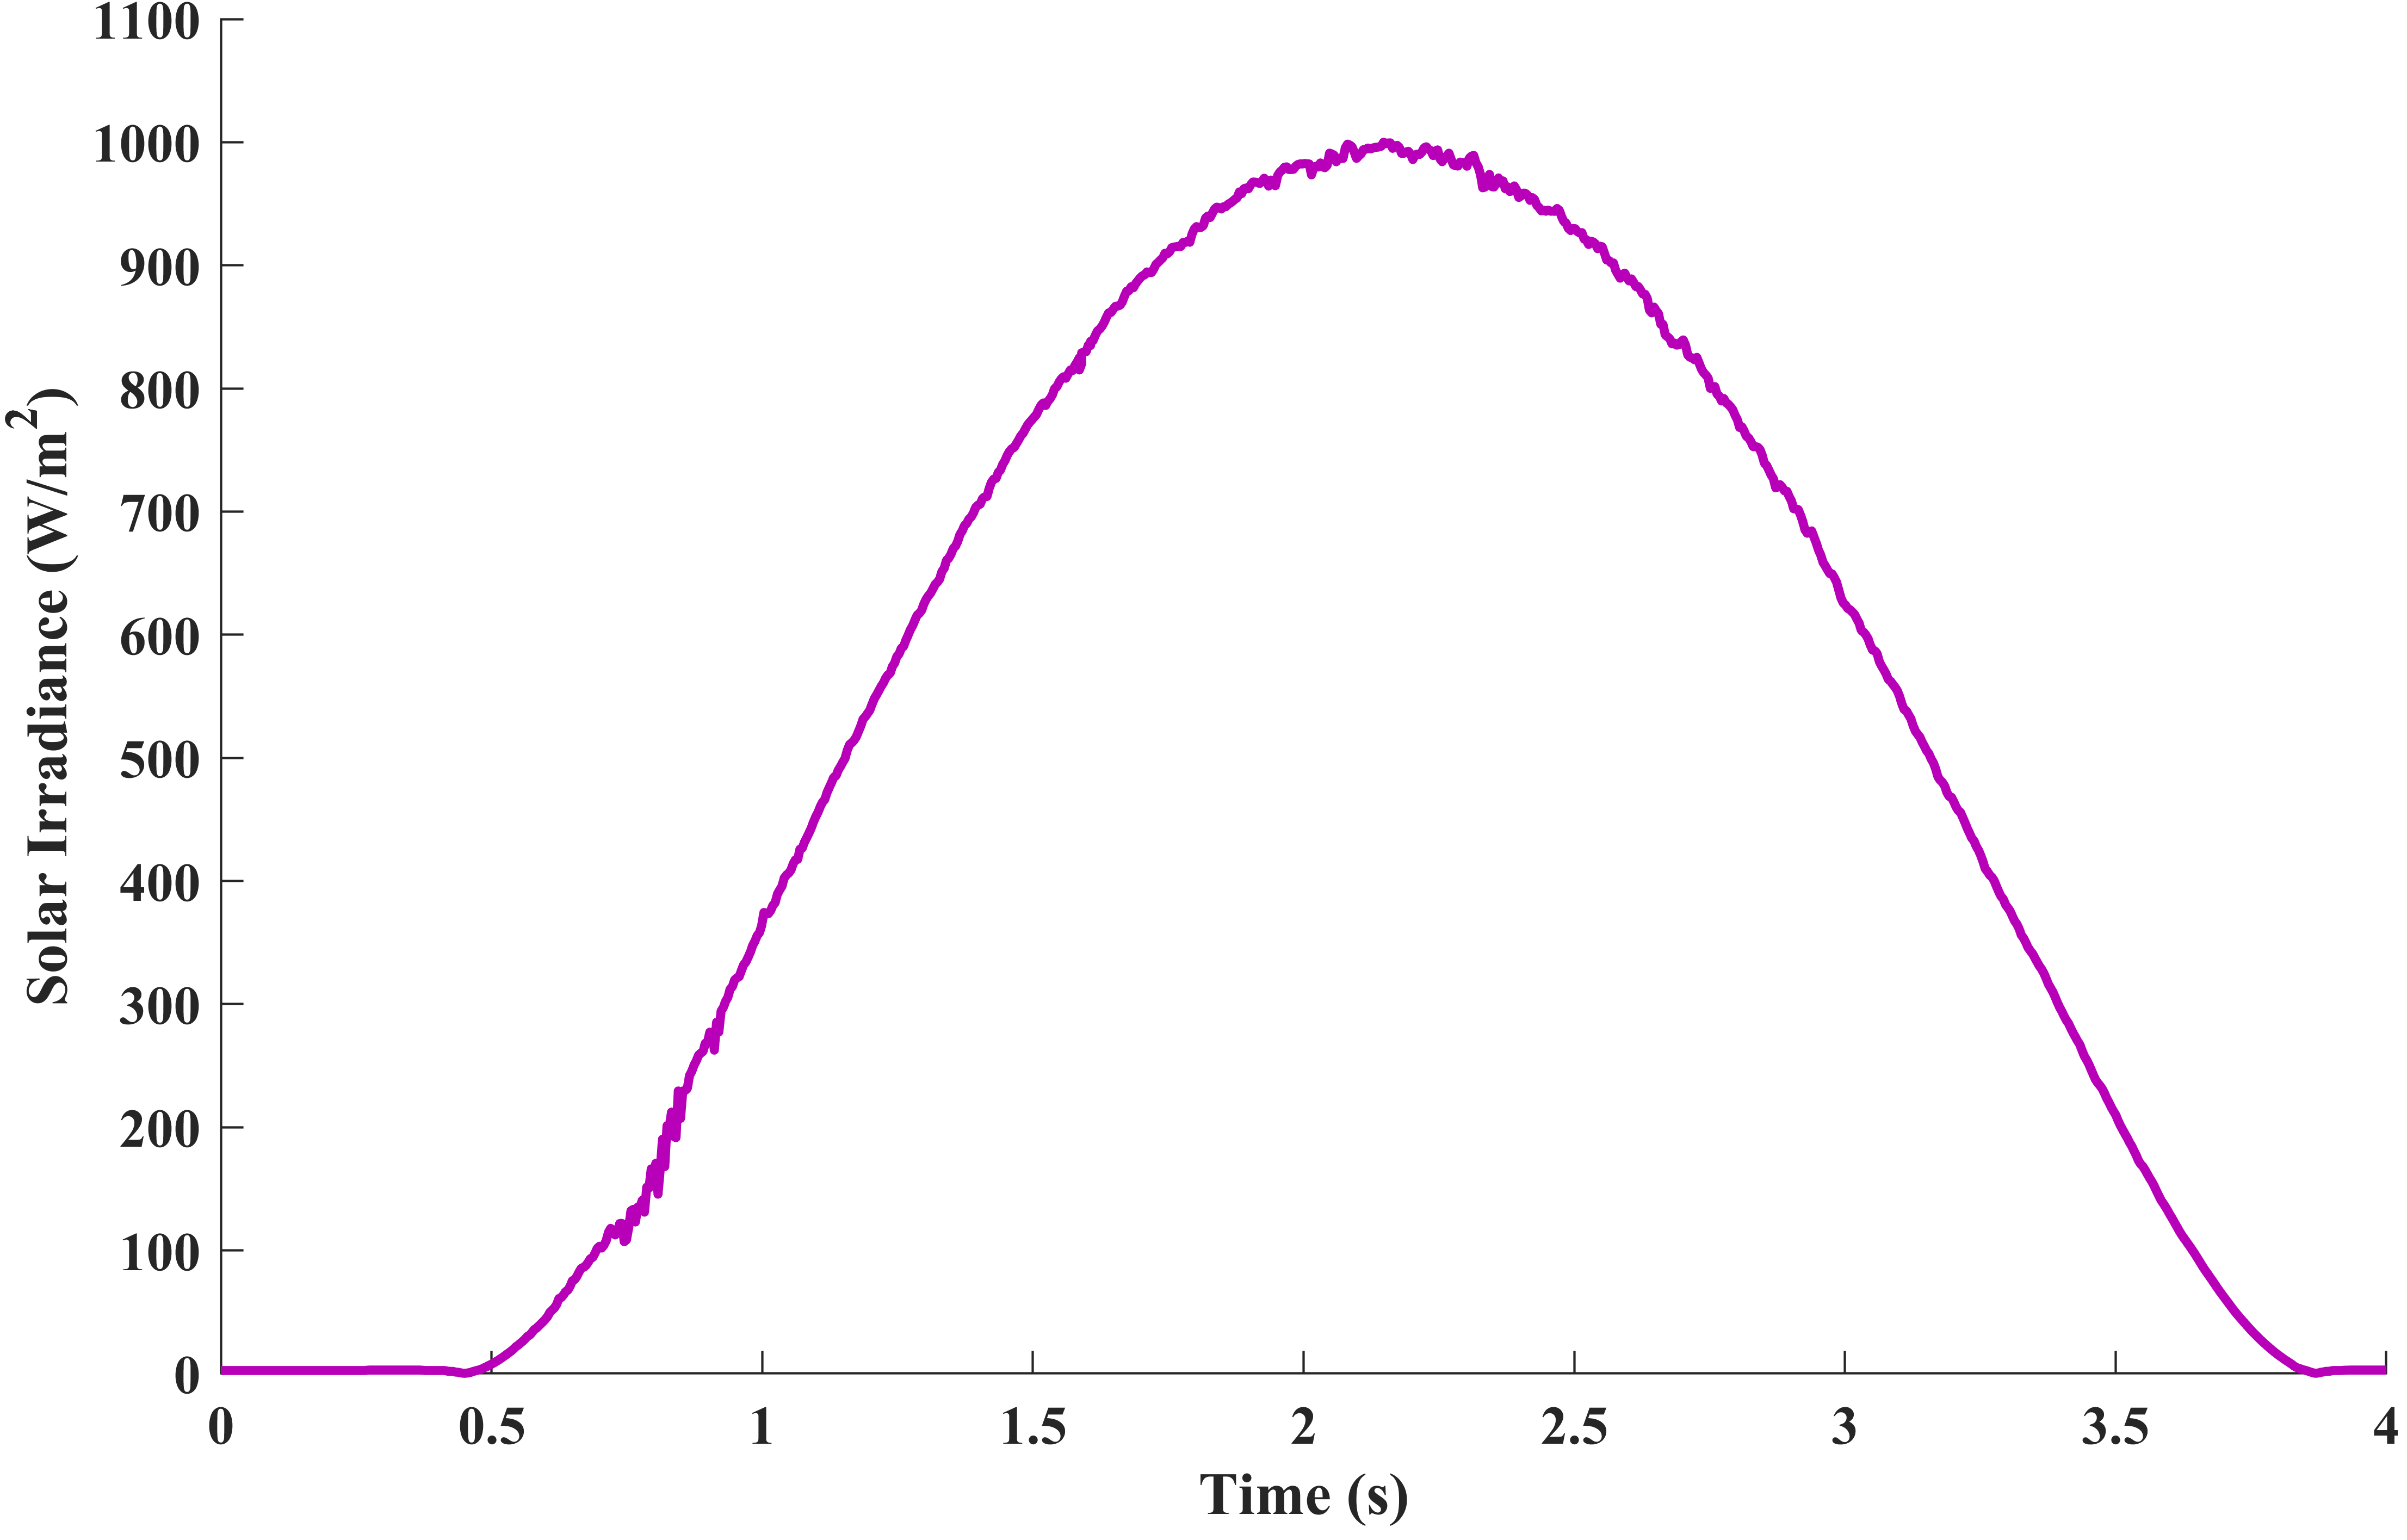
\includegraphics[width=.90\columnwidth]{Pictures/SOLAR IRREDIANCE.png}
\caption{{Solar irradiance curve {\label{fig:irradiance-profile}}%
}}
\end{center}
\end{figure}
\subsubsection{Simulation results of Proposed Controllers}
The performance of the Continuous Twisting Algorithm Sliding Mode Controller (CTA-SMC) and Discontinuous Integral Controller Sliding Mode Controller (DIC-SMC) were evaluated using key attributes of the PV system, including PV voltage, current, irradiance, and MPPT curve. This section assesses the controller’s ability to regulate the DC-link voltage, output current, active/reactive power, and Total Harmonic Distortion (THD). Additionally, grid-side metrics, such as the power factor and voltage-current phase synchronization, were analyzed to comprehensively compare the efficacy of the CTA-SMC and (DIC-SMC) PI Control strategies.
\subsection{Controllers Results}
Both CTA-SMC and DIC-SMC demonstrated robust control in grid-connected PV systems. The CTA-SMC (Fig.~\ref{fig:sliding-surfaces}(a) and (c)) achieves rapid stabilization with minimal fluctuations, excelling in the dynamic response to varying irradiance. In contrast, DIC-SMC (Fig.  The sliding surfaces in Figs. ~\ref{fig:sliding-surfaces}(b) and (d)) exhibit marginally slower transient behaviors but ensure stable operation with negligible overshoot and oscillations, even under abrupt load changes. While CTA-SMC prioritizes agility, DIC-SMC emphasizes precision in the steady state. These results underscore the suitability of these devices for real-world applications that demand high power quality and resilience.
\begin{figure}
    \centering
    % First row of images
    \begin{subfigure}{0.45\textwidth}
        \centering
        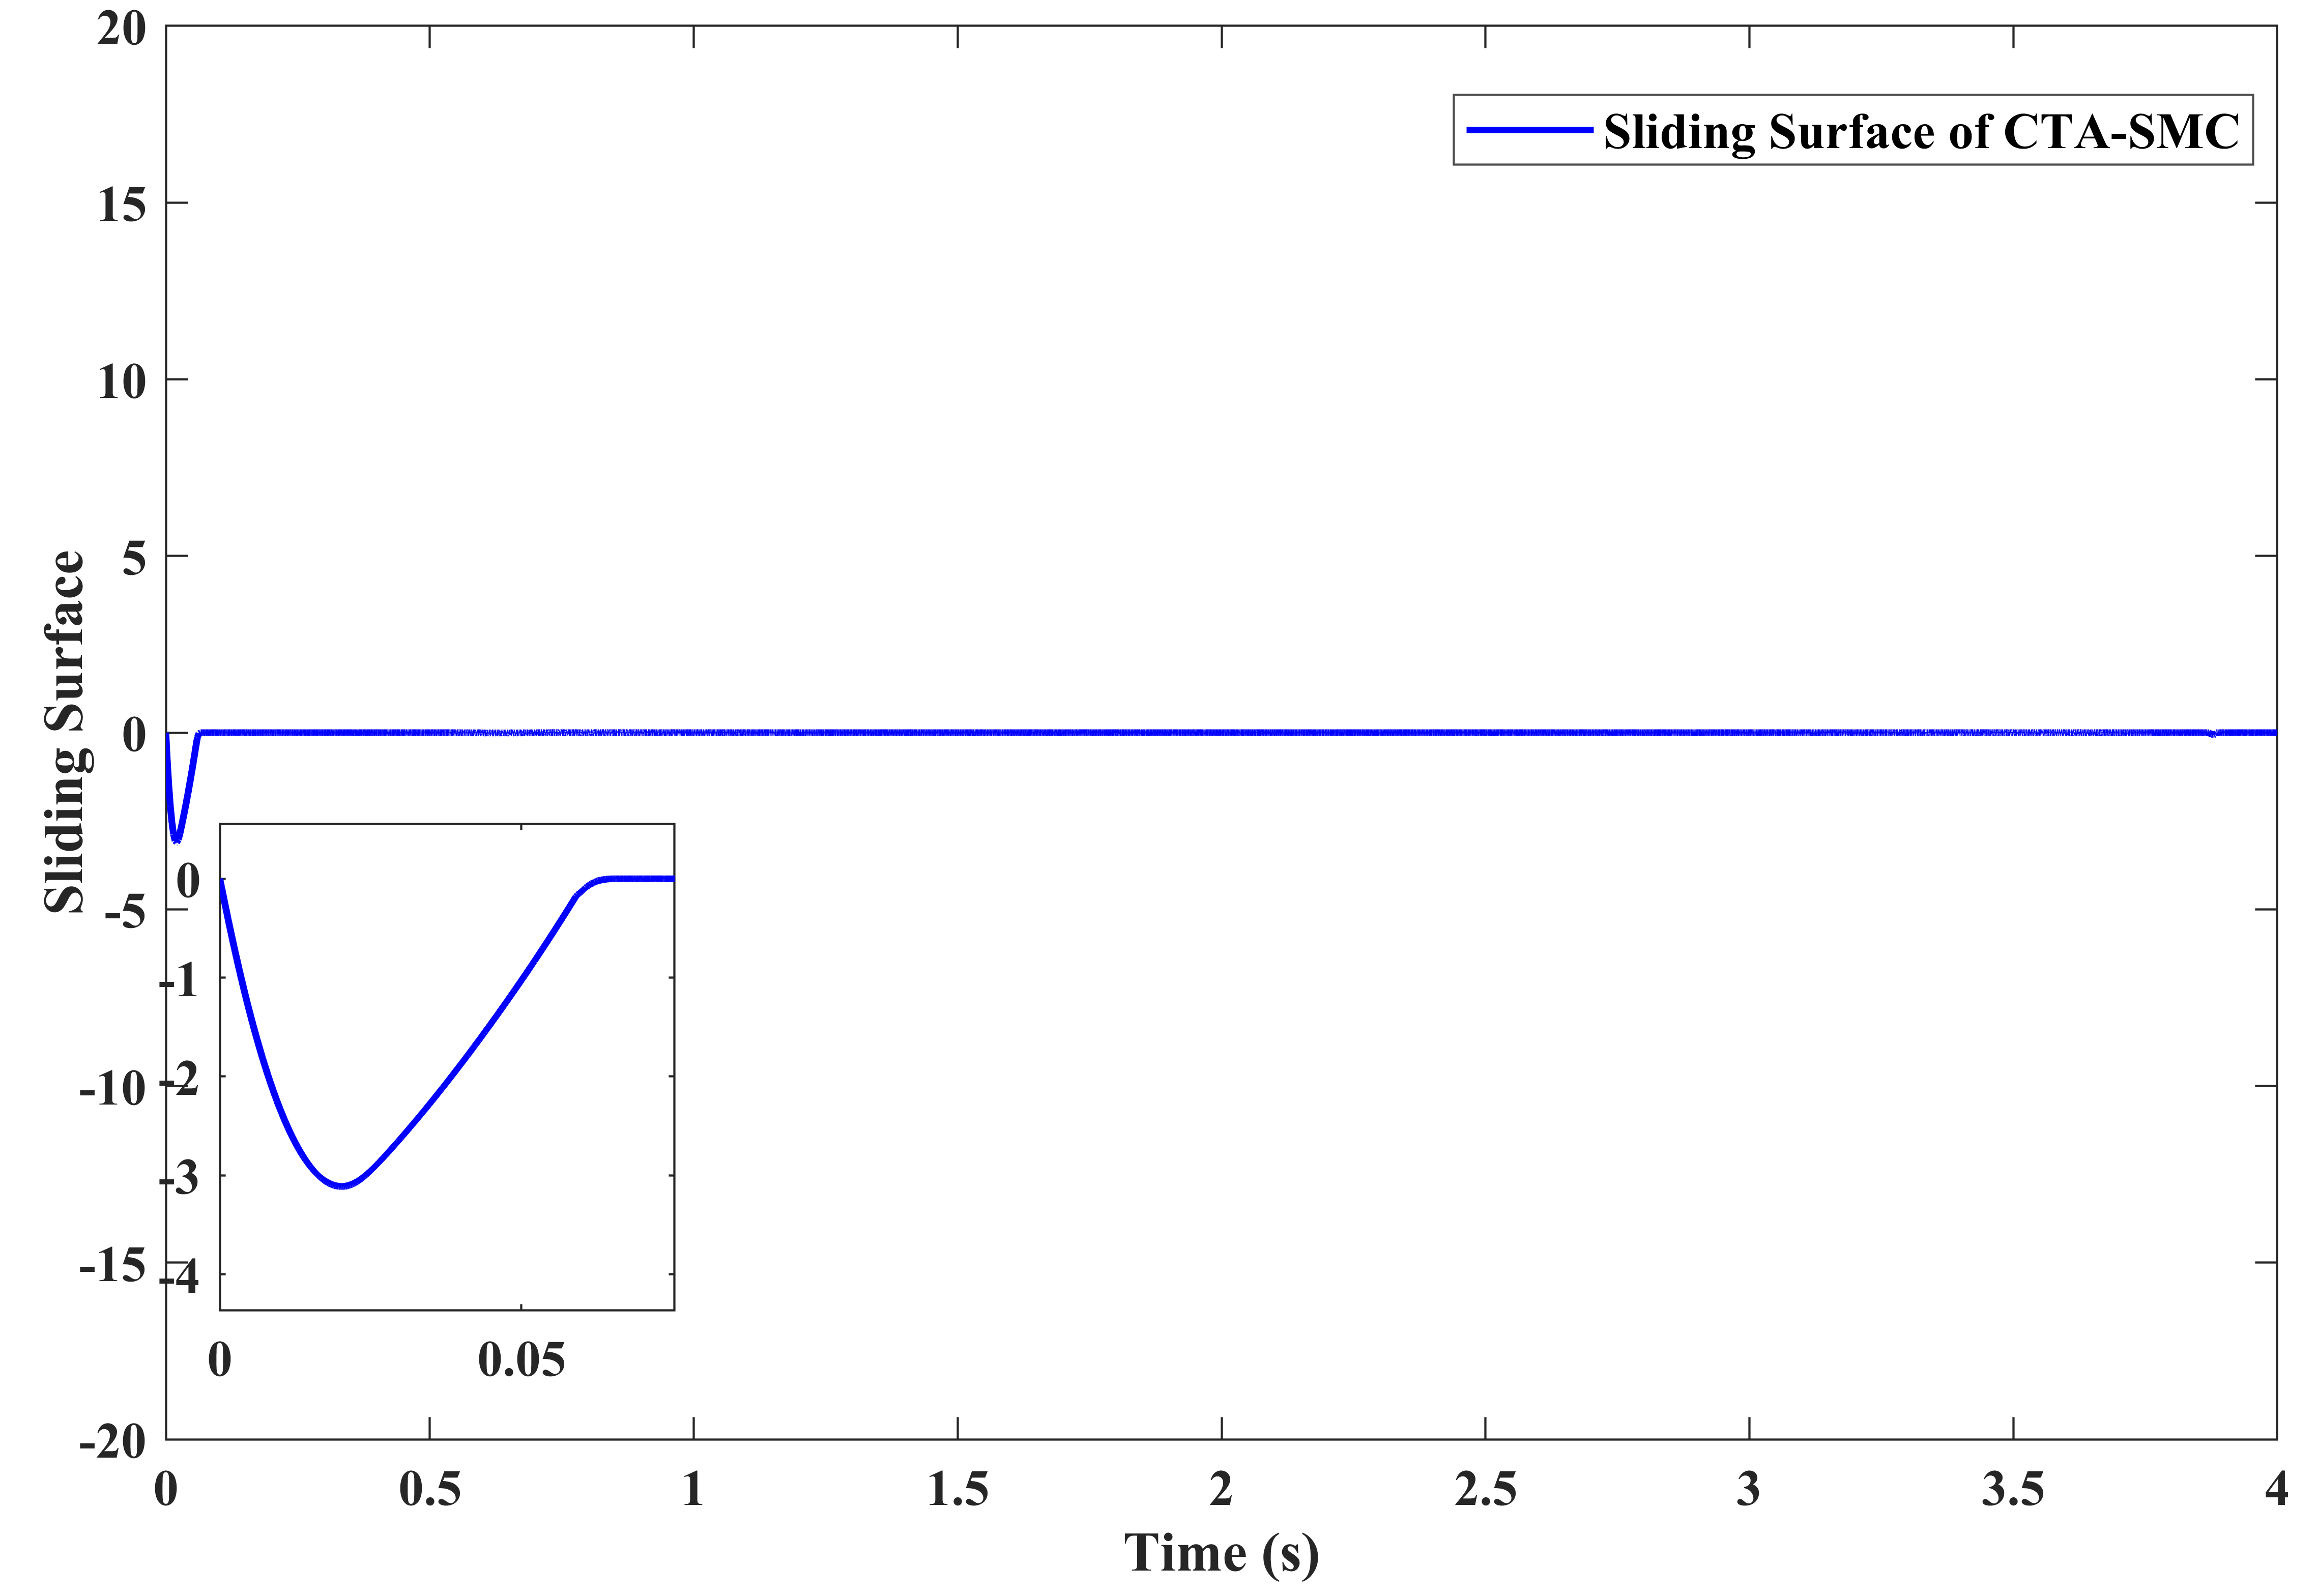
\includegraphics[width=\textwidth, height=4cm, keepaspectratio]{Pictures/CTA Sliding Surface MPPT.png}
        \caption{Sliding surface of MPPT CTA Controller}
    \end{subfigure}
    \hfill
    \begin{subfigure}{0.45\textwidth}
        \centering
        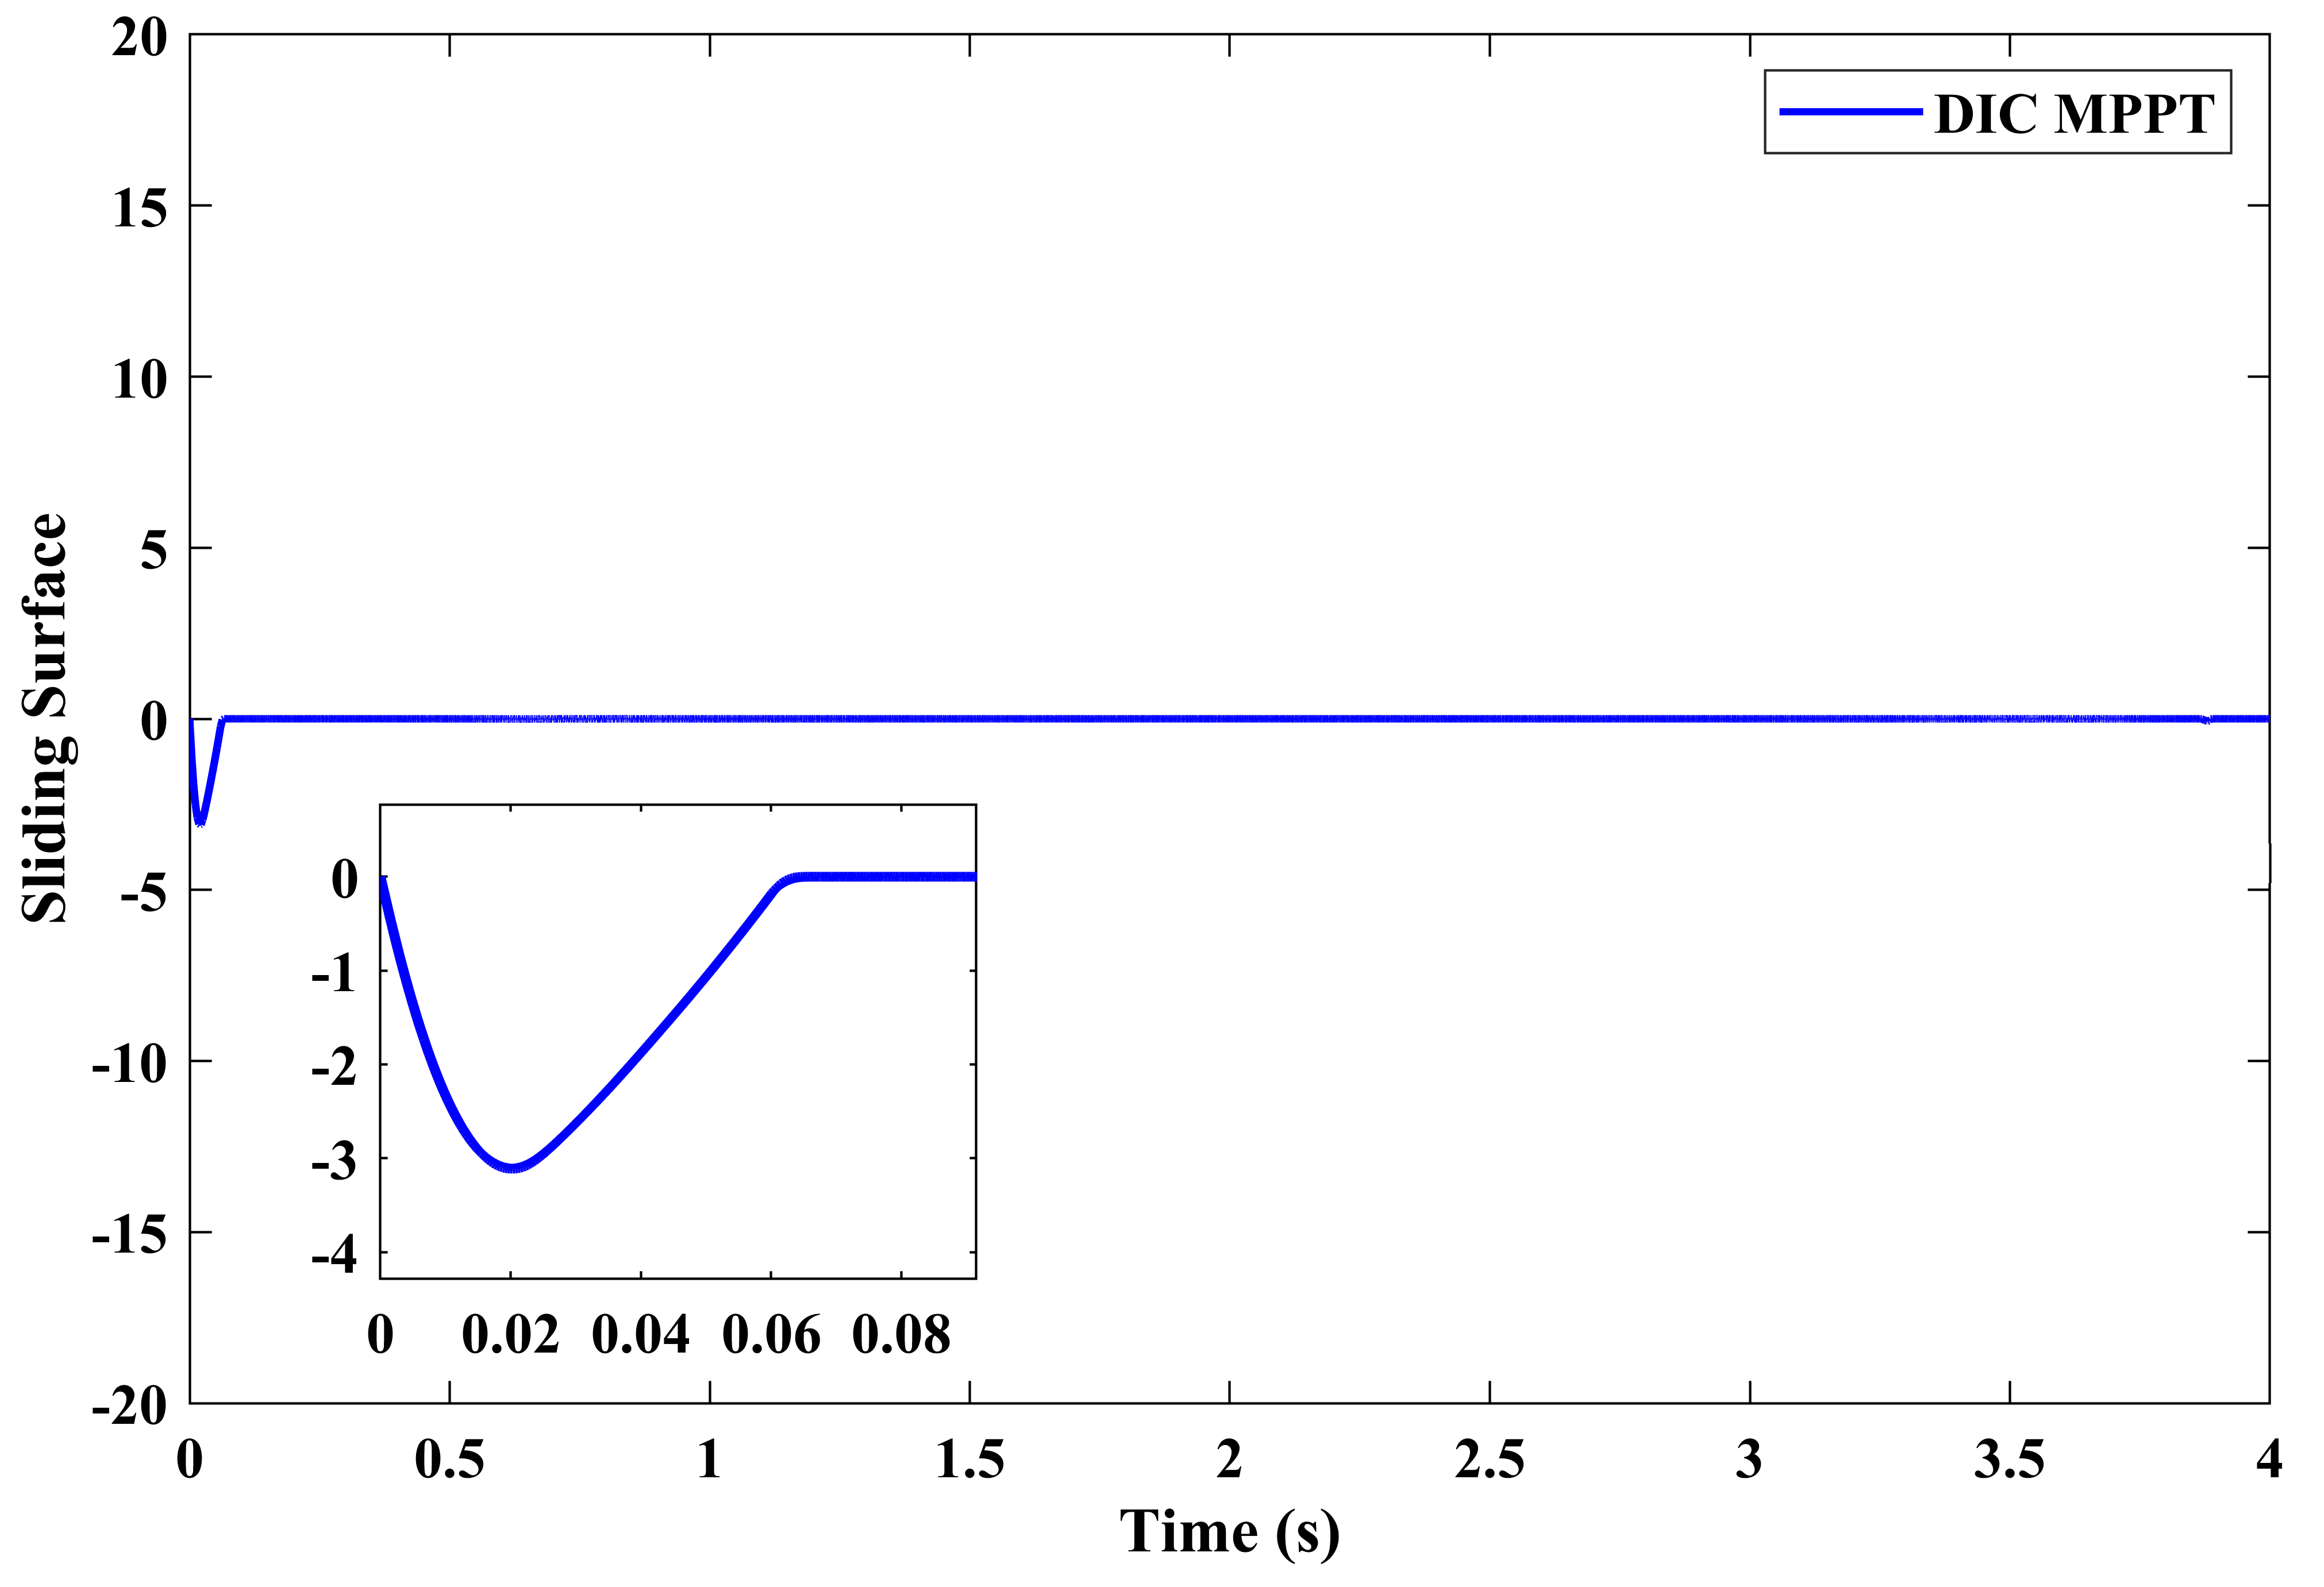
\includegraphics[width=\textwidth, height=4cm, keepaspectratio]{Pictures/Sliding surface DIC mppt.png}
        \caption{Sliding surface of MPPT DIC controller}
    \end{subfigure}
      % Second row of images
\begin{subfigure}{0.45\textwidth}
        \centering
        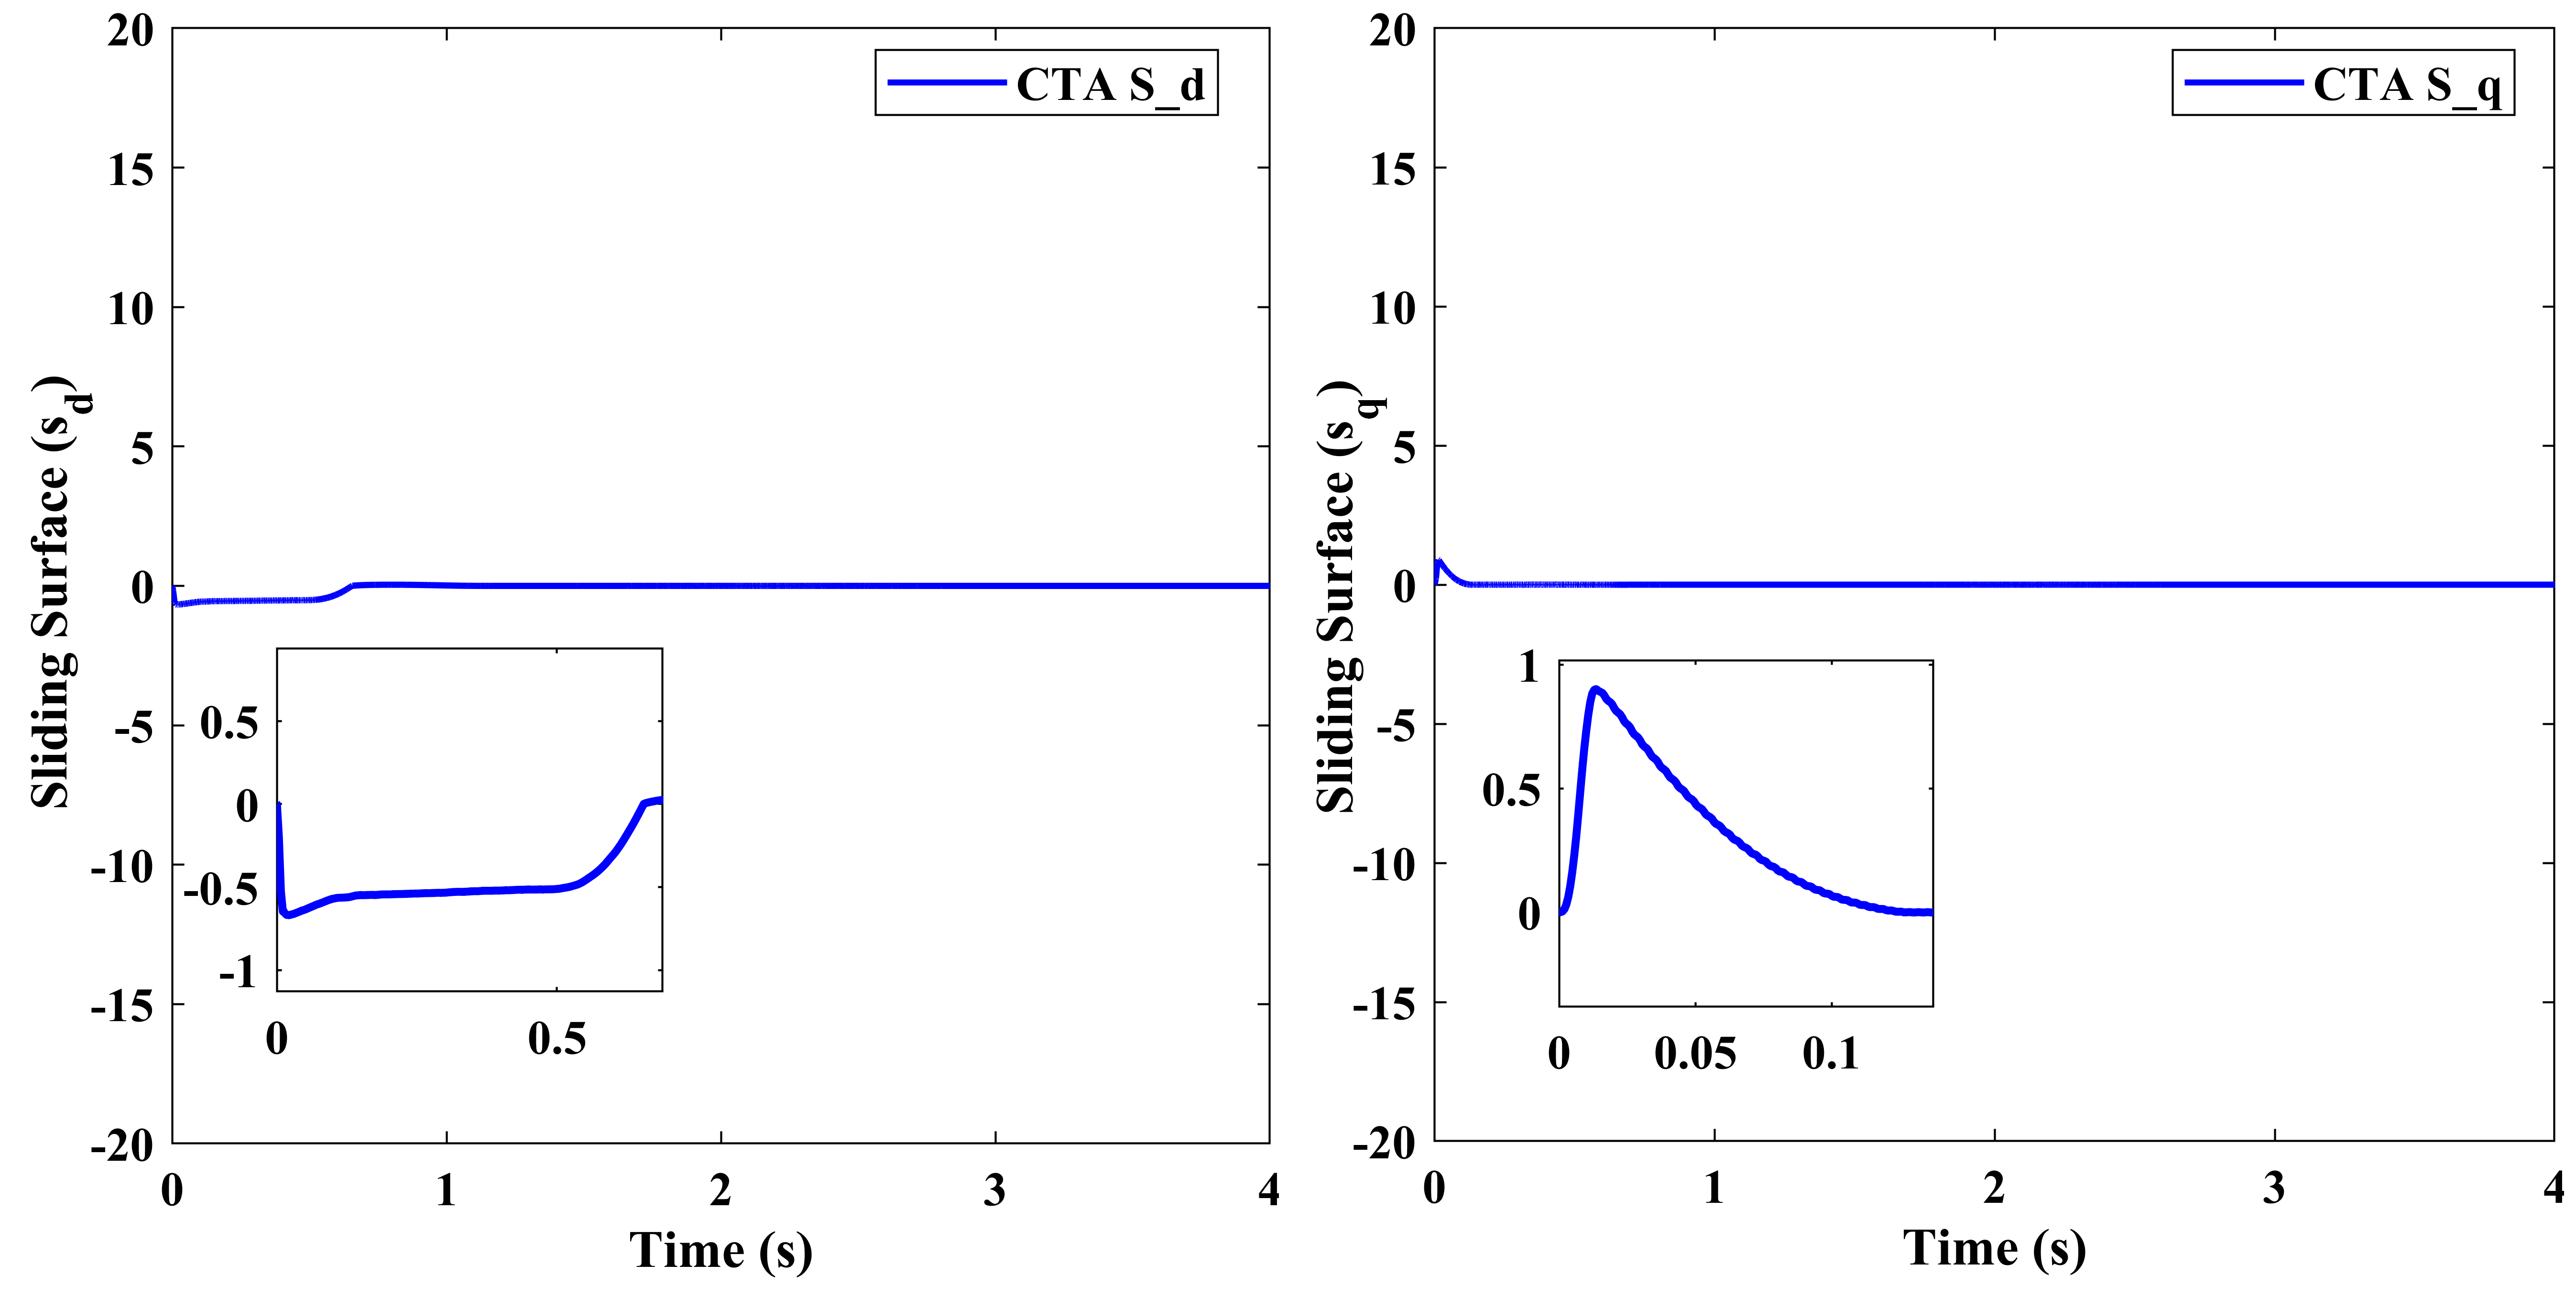
\includegraphics[width=\textwidth, height=4cm, keepaspectratio]{Pictures/Sliding Surface CTA Inverter.png}
        \caption{Sliding surface of Inverter CTA controller}
    \end{subfigure}
    \hfill
    \begin{subfigure}{0.45\textwidth}
        \centering
        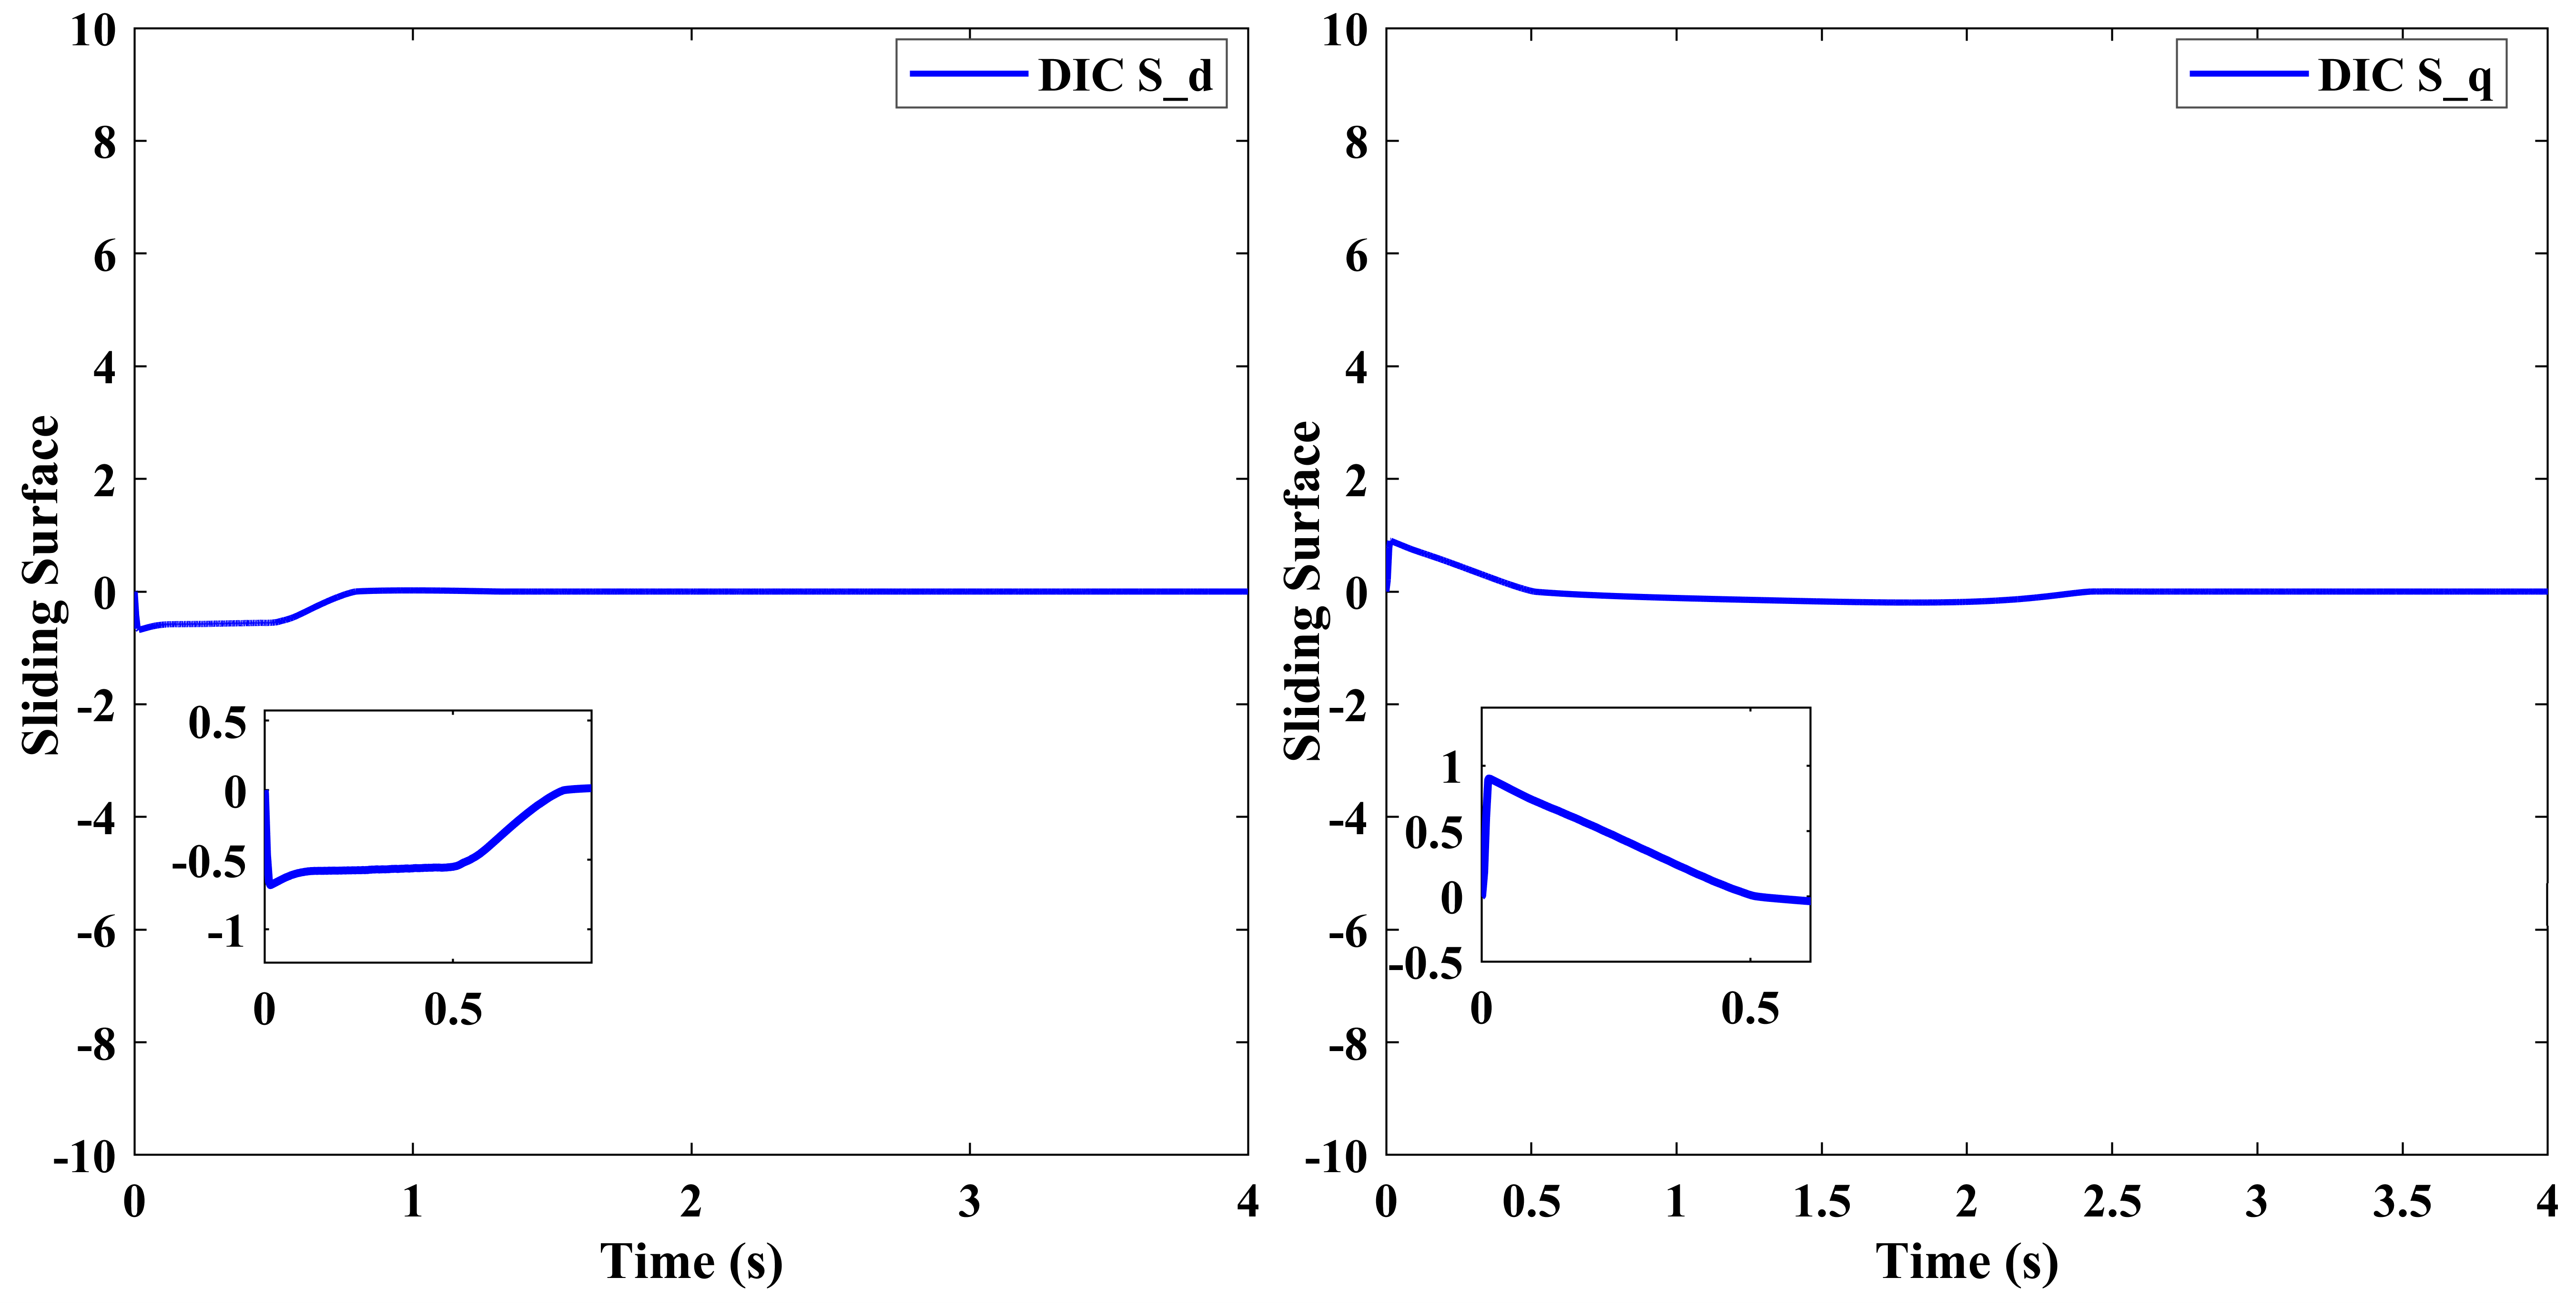
\includegraphics[width=\textwidth, height=4cm, keepaspectratio]{Pictures/Sliding Surface DIC Inverter.png}
        \caption{Sliding surface of inverter DIC controller}
    \end{subfigure}
    
    \caption{Sliding surfaces of the proposed MPPT and inverter controllers .}
    \label{fig:sliding-surfaces}
\end{figure}

\subsection{Results of Utkin Observer}
Accurate estimation of internal states, such as filter capacitor voltage and inverter current, is critical for optimizing the control performance and ensuring stability in grid-tied PV systems. Building on the framework derived in Section 3, a Utkin sliding mode observer was implemented to estimate these states in the dq reference frame by leveraging the measured grid currents. This observer excels in uncertain or disturbed environments (e.g., grid fluctuations or parameter variations) owing to its inherent robustness, whereas the dq transformation streamlines the system dynamics for improved real-time compatibility.

The observer efficacy is shown in Fig. ~\ref{fig:observer-results}, which compares the estimated and actual values of the capacitor voltage, inverter current, and grid current in dq coordinates. The results demonstrate high-precision state estimation, enabling sensor reduction and enhancing the reliability of control strategies for grid-connected PV systems.


\begin{figure}
    \centering
    % First row of images
    \begin{subfigure}{0.45\textwidth}
        \centering
        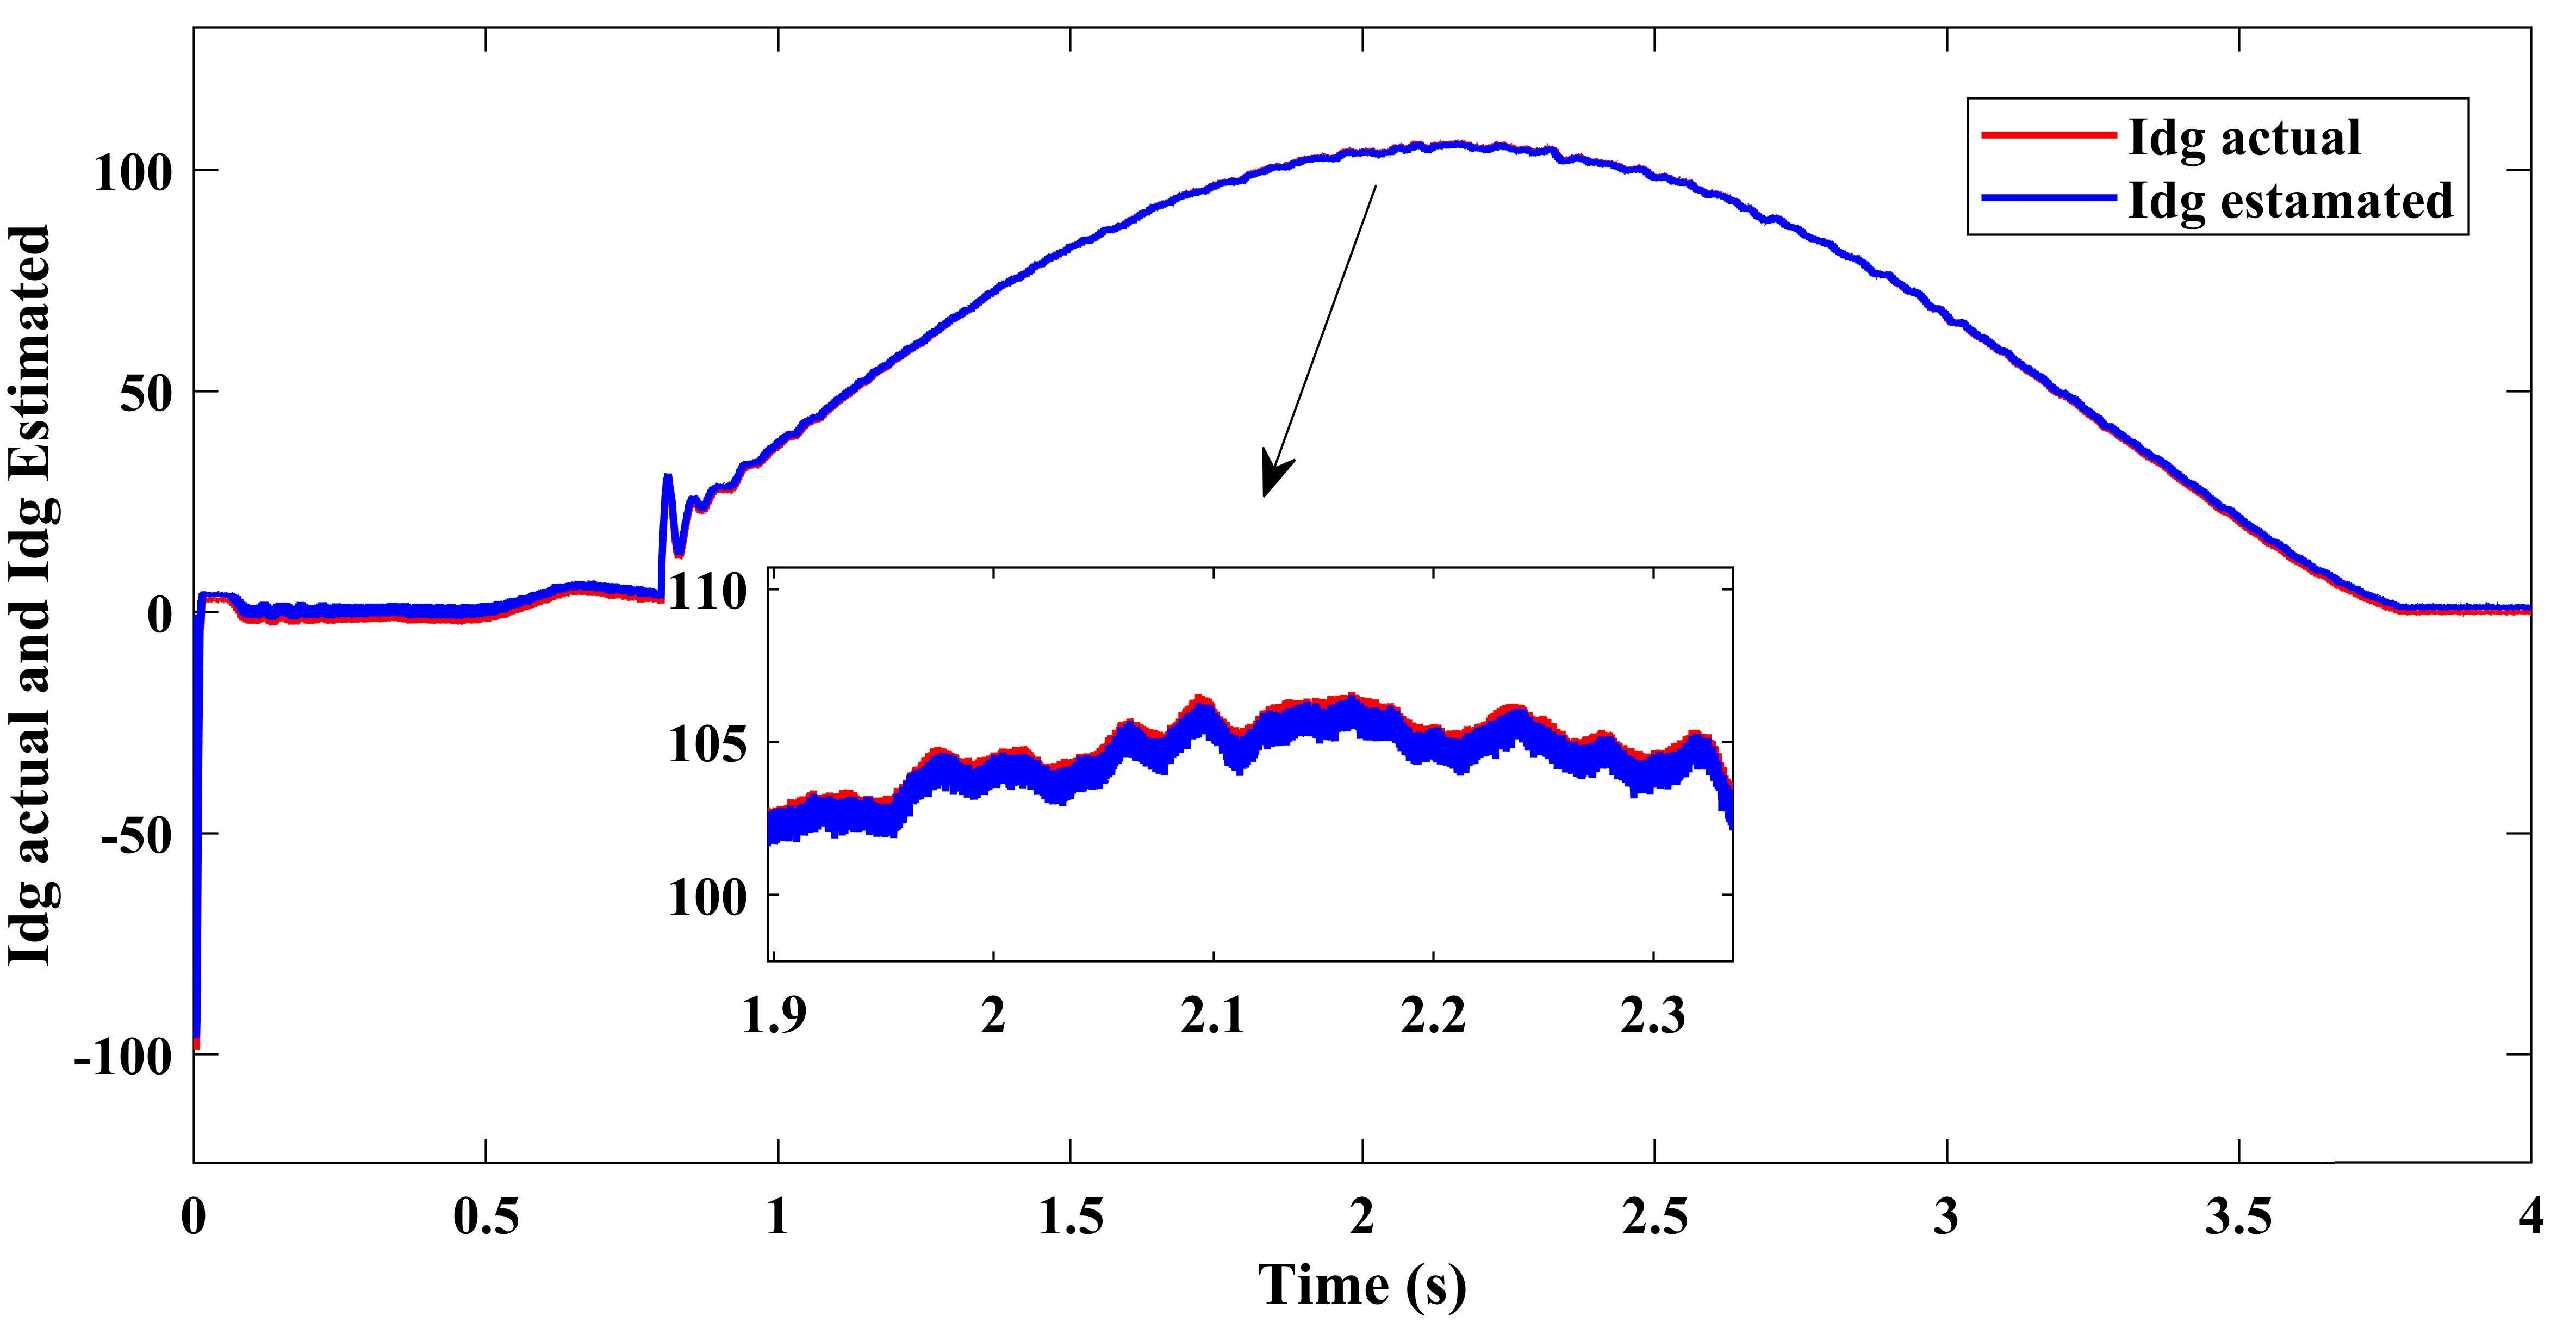
\includegraphics[width=\textwidth, height=4cm]{Pictures/Igd Observed.jpg}
        \caption{Grid current $I_{gd}$: estimated vs. actual}
    \end{subfigure}
    \hfill
    \begin{subfigure}{0.45\textwidth}
        \centering
        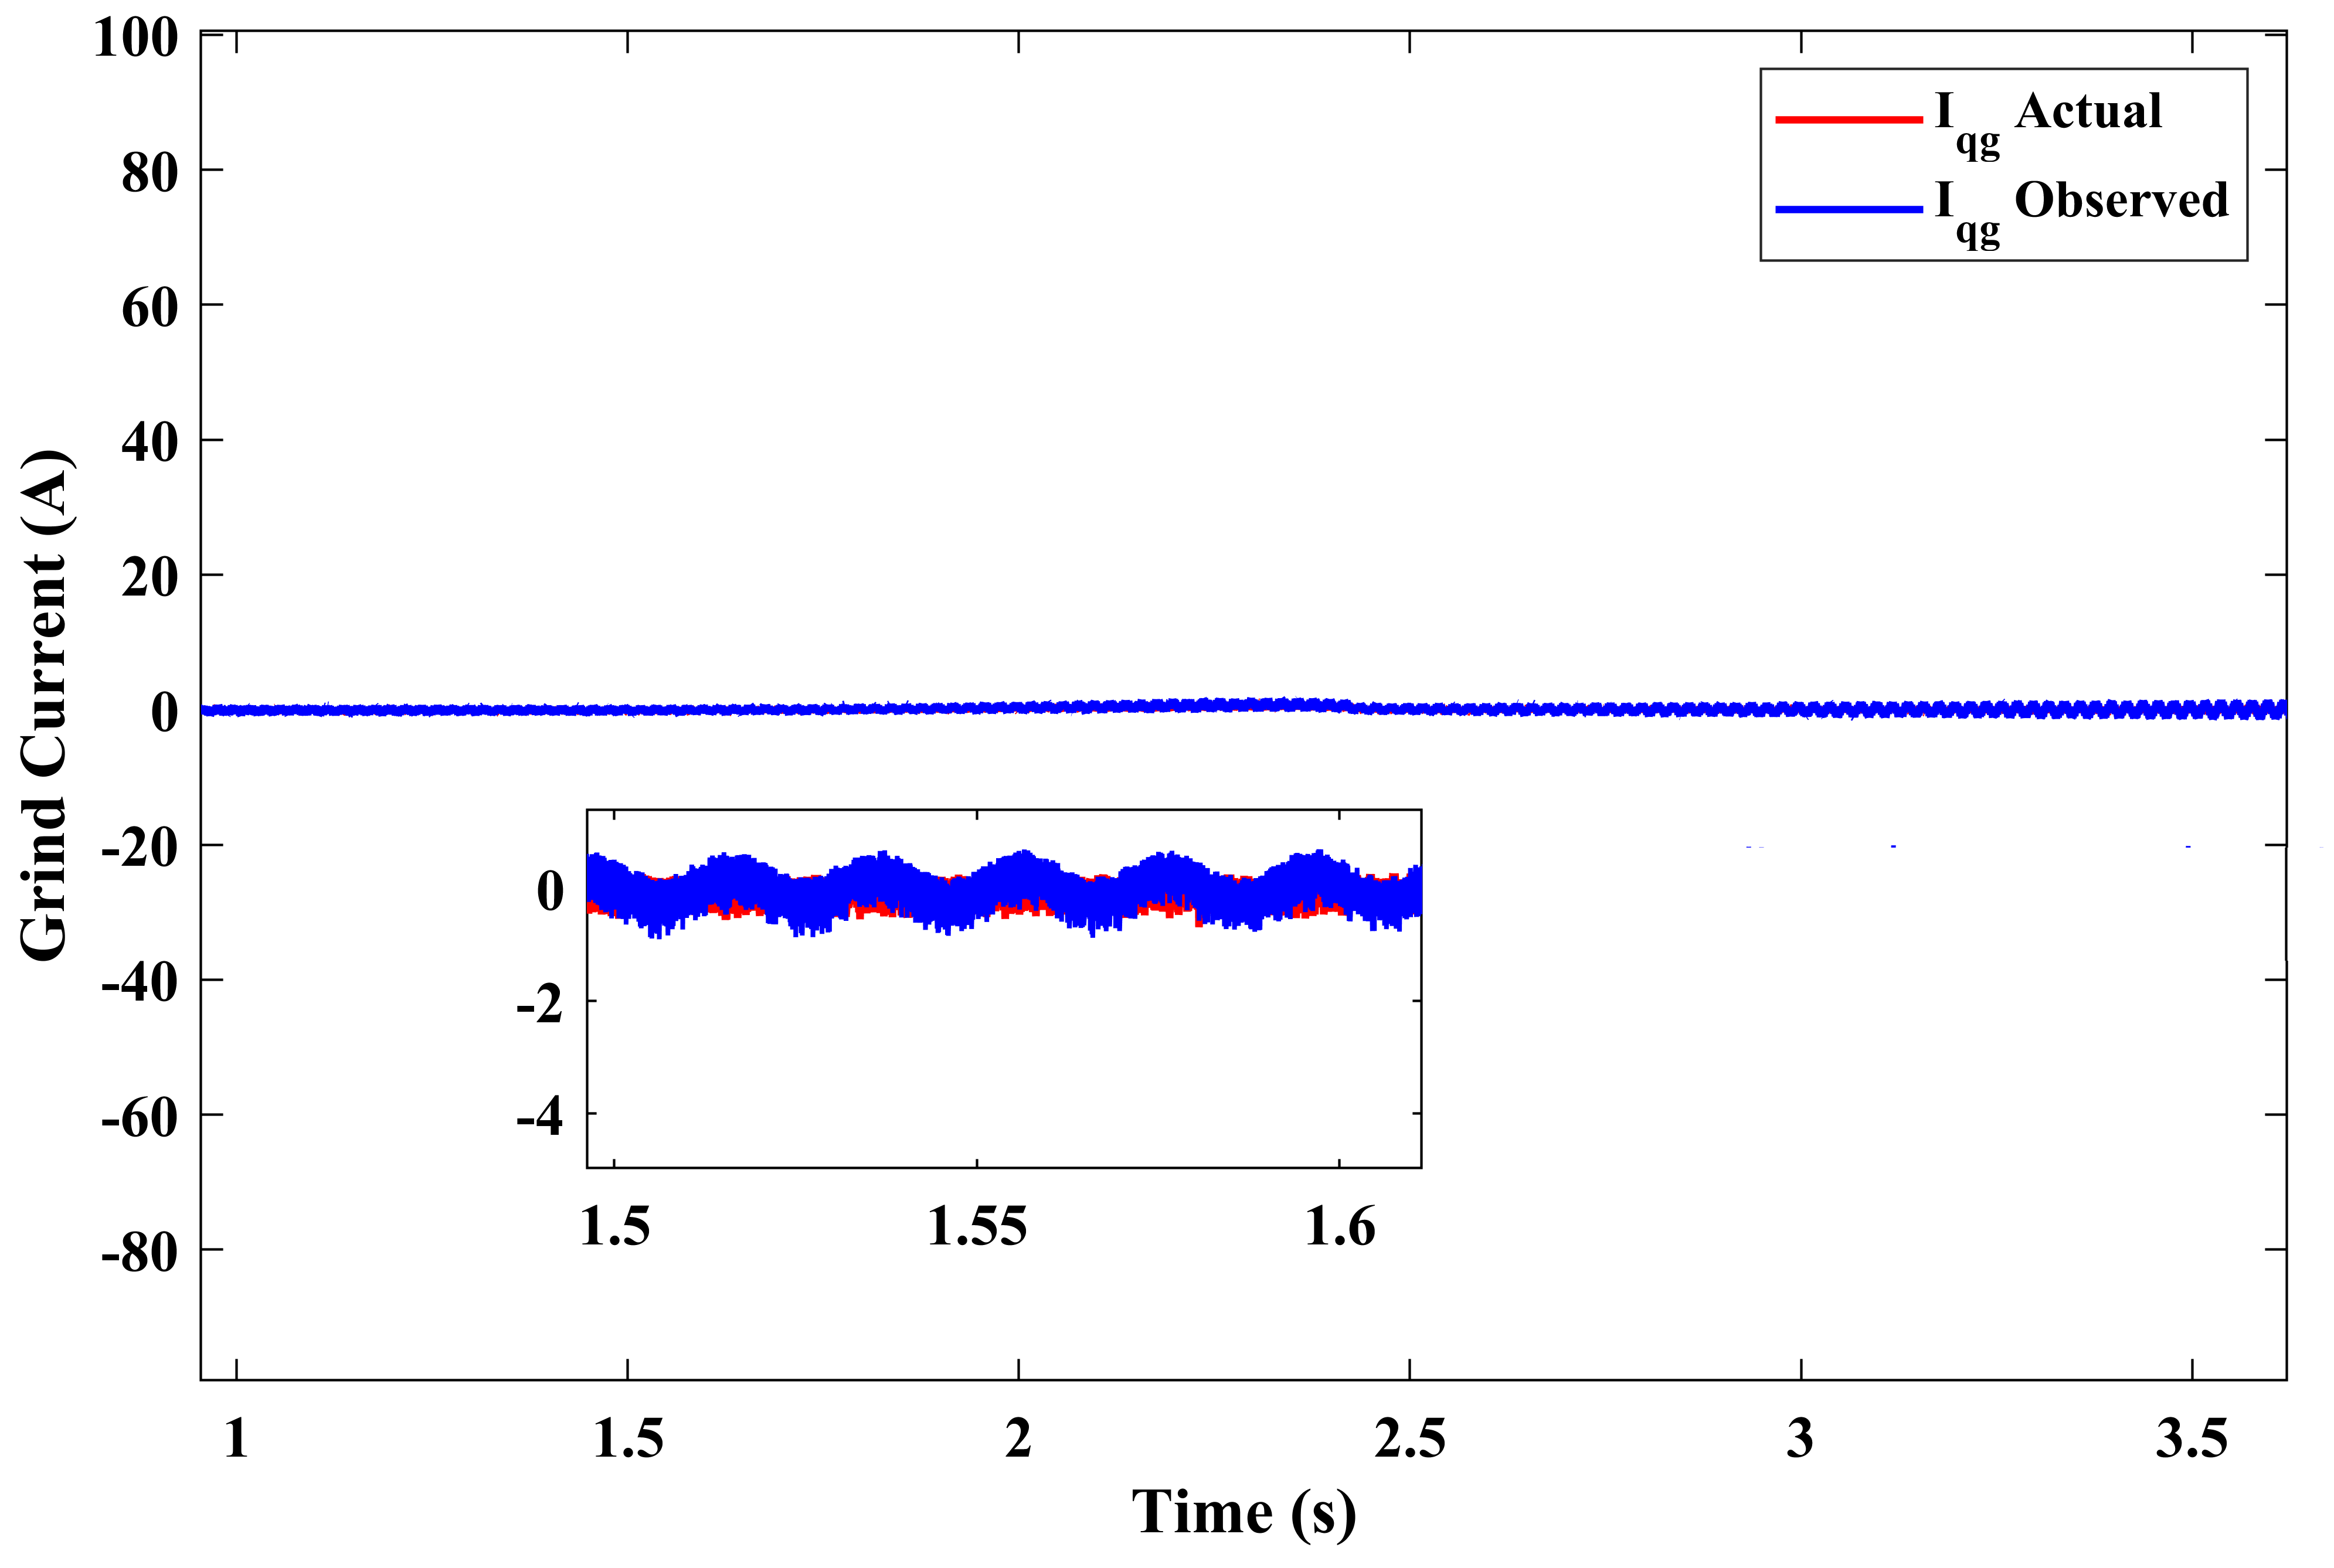
\includegraphics[width=\textwidth, height=4cm]{Pictures/Igq Observed.png}
        \caption{Grid current $I_{gq}$: estimated vs. actual}
    \end{subfigure}

    % Second row of images
    \begin{subfigure}{0.45\textwidth}
        \centering
        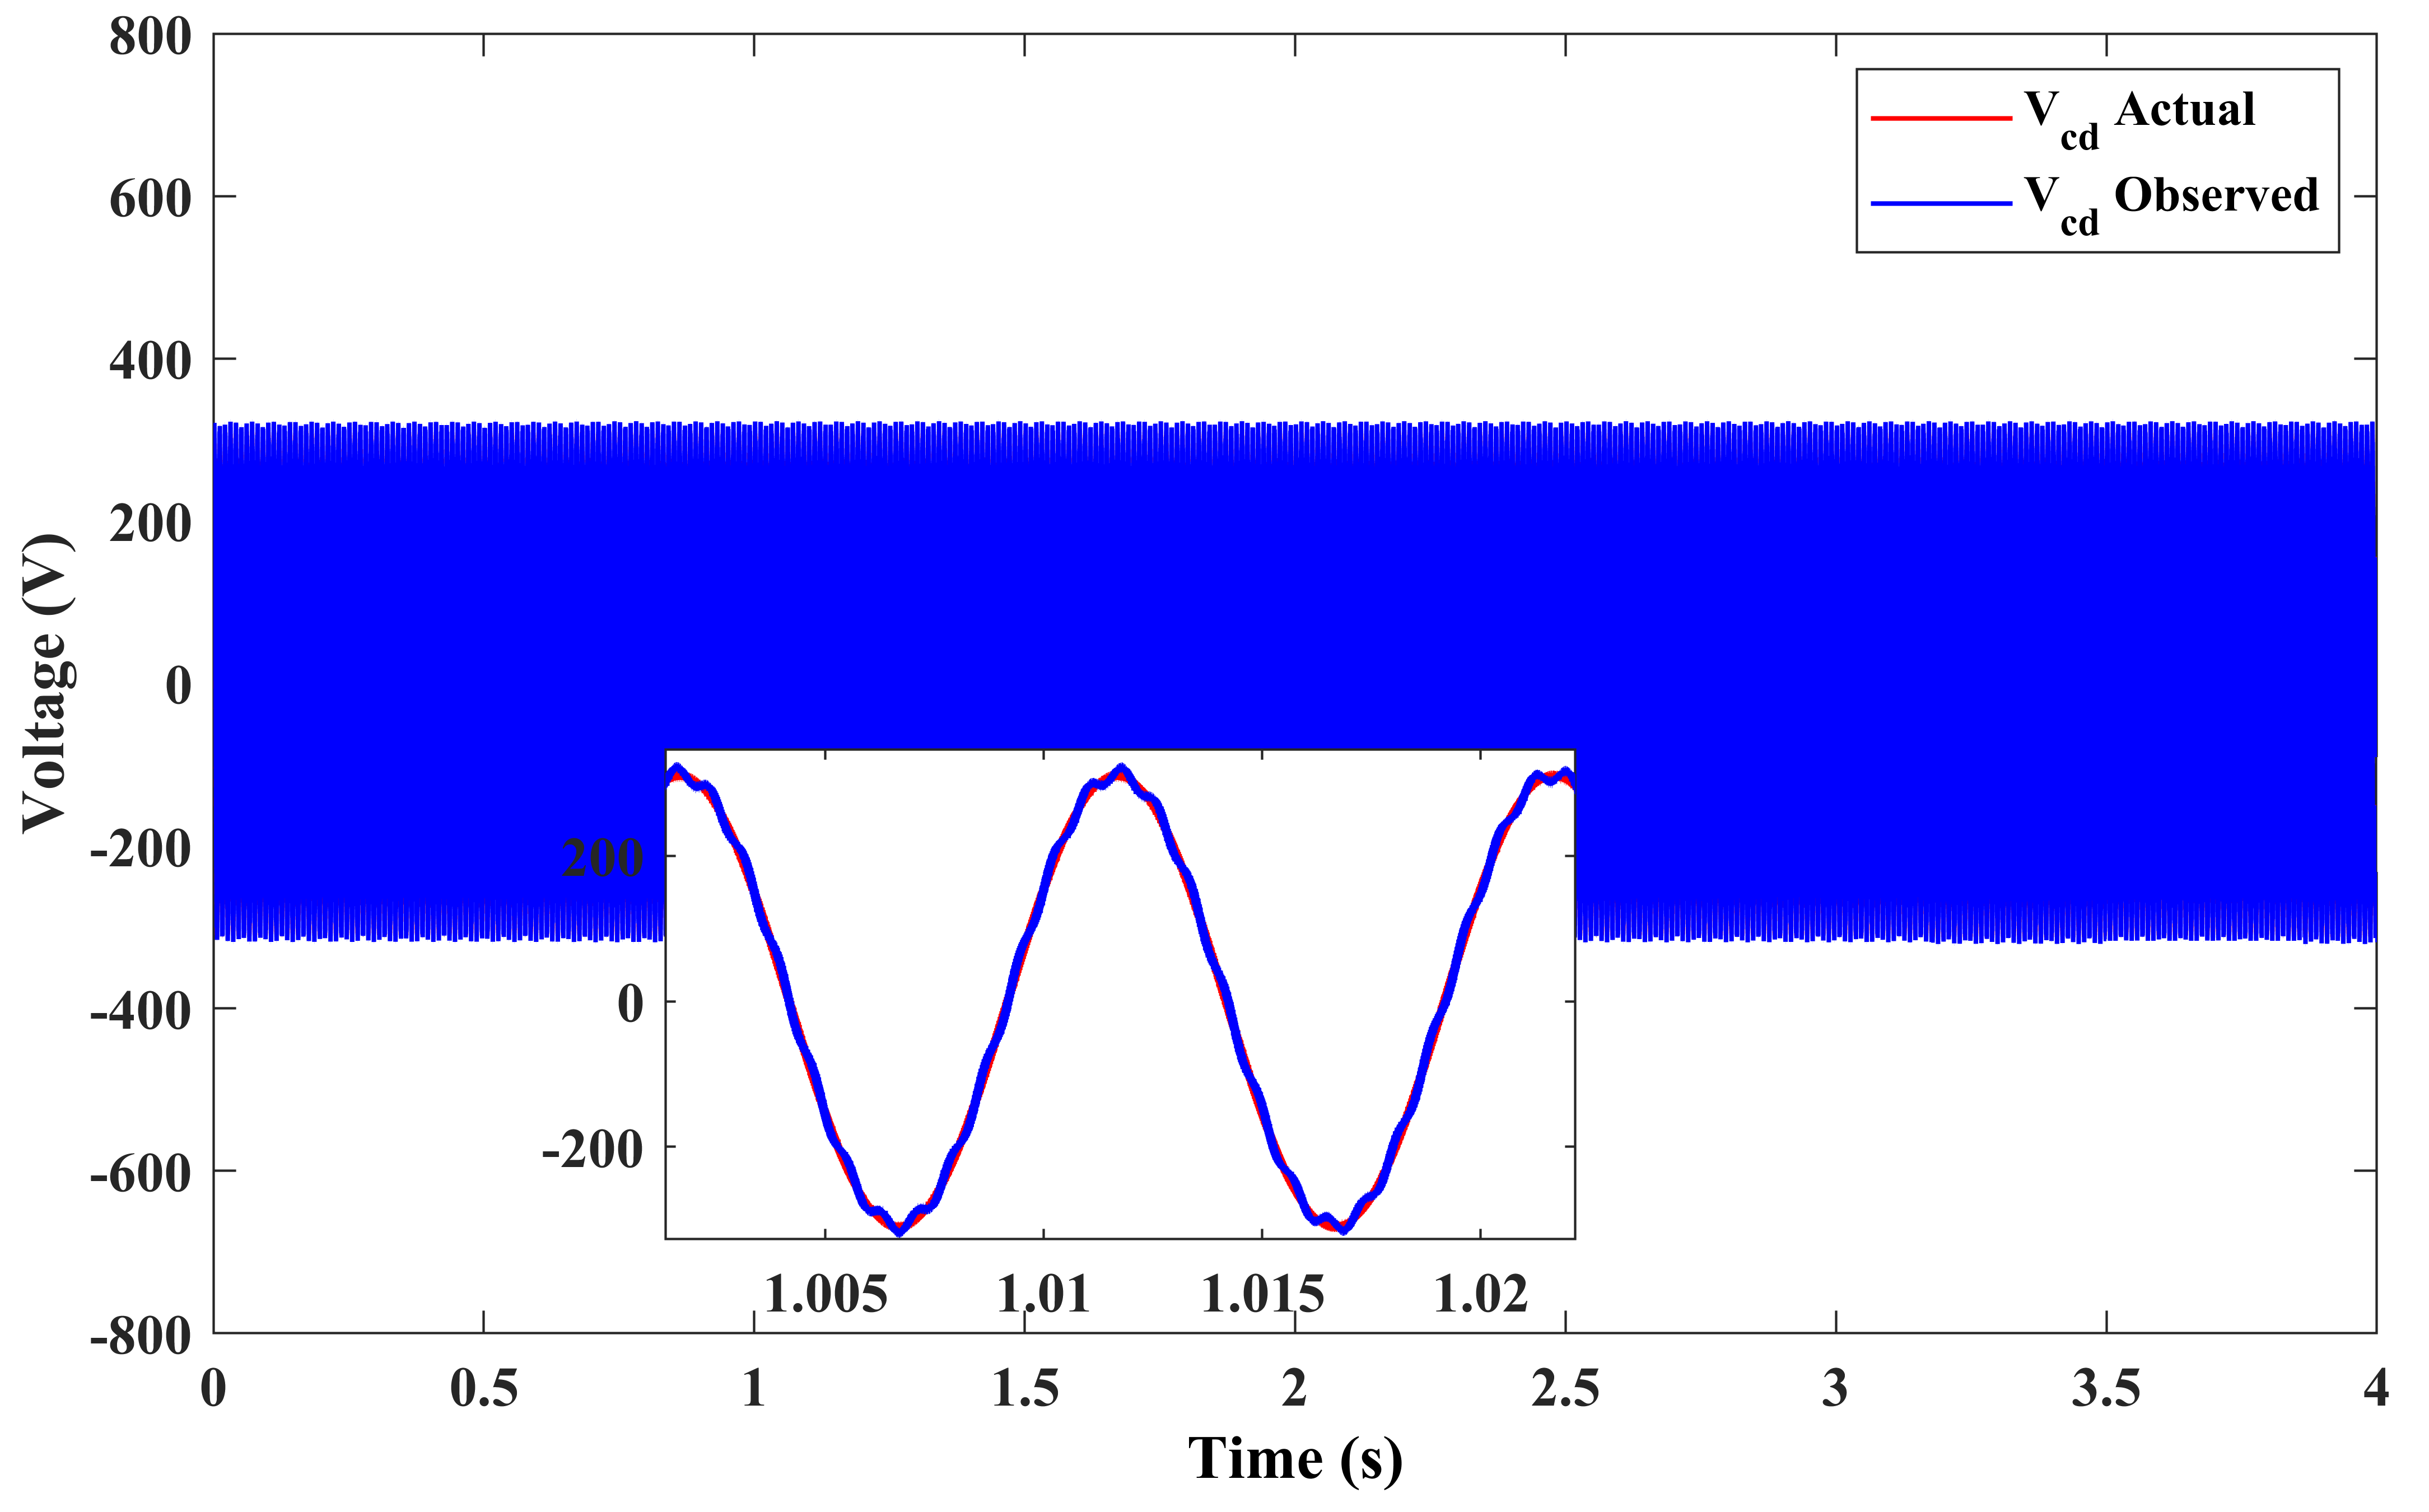
\includegraphics[width=\textwidth, height=4cm]{Pictures/Vcd Observed New1.png}
        \caption{Capacitor voltage $V_{cd}$: estimated vs. actual}
    \end{subfigure}
    \hfill
    \begin{subfigure}{0.45\textwidth}
        \centering
        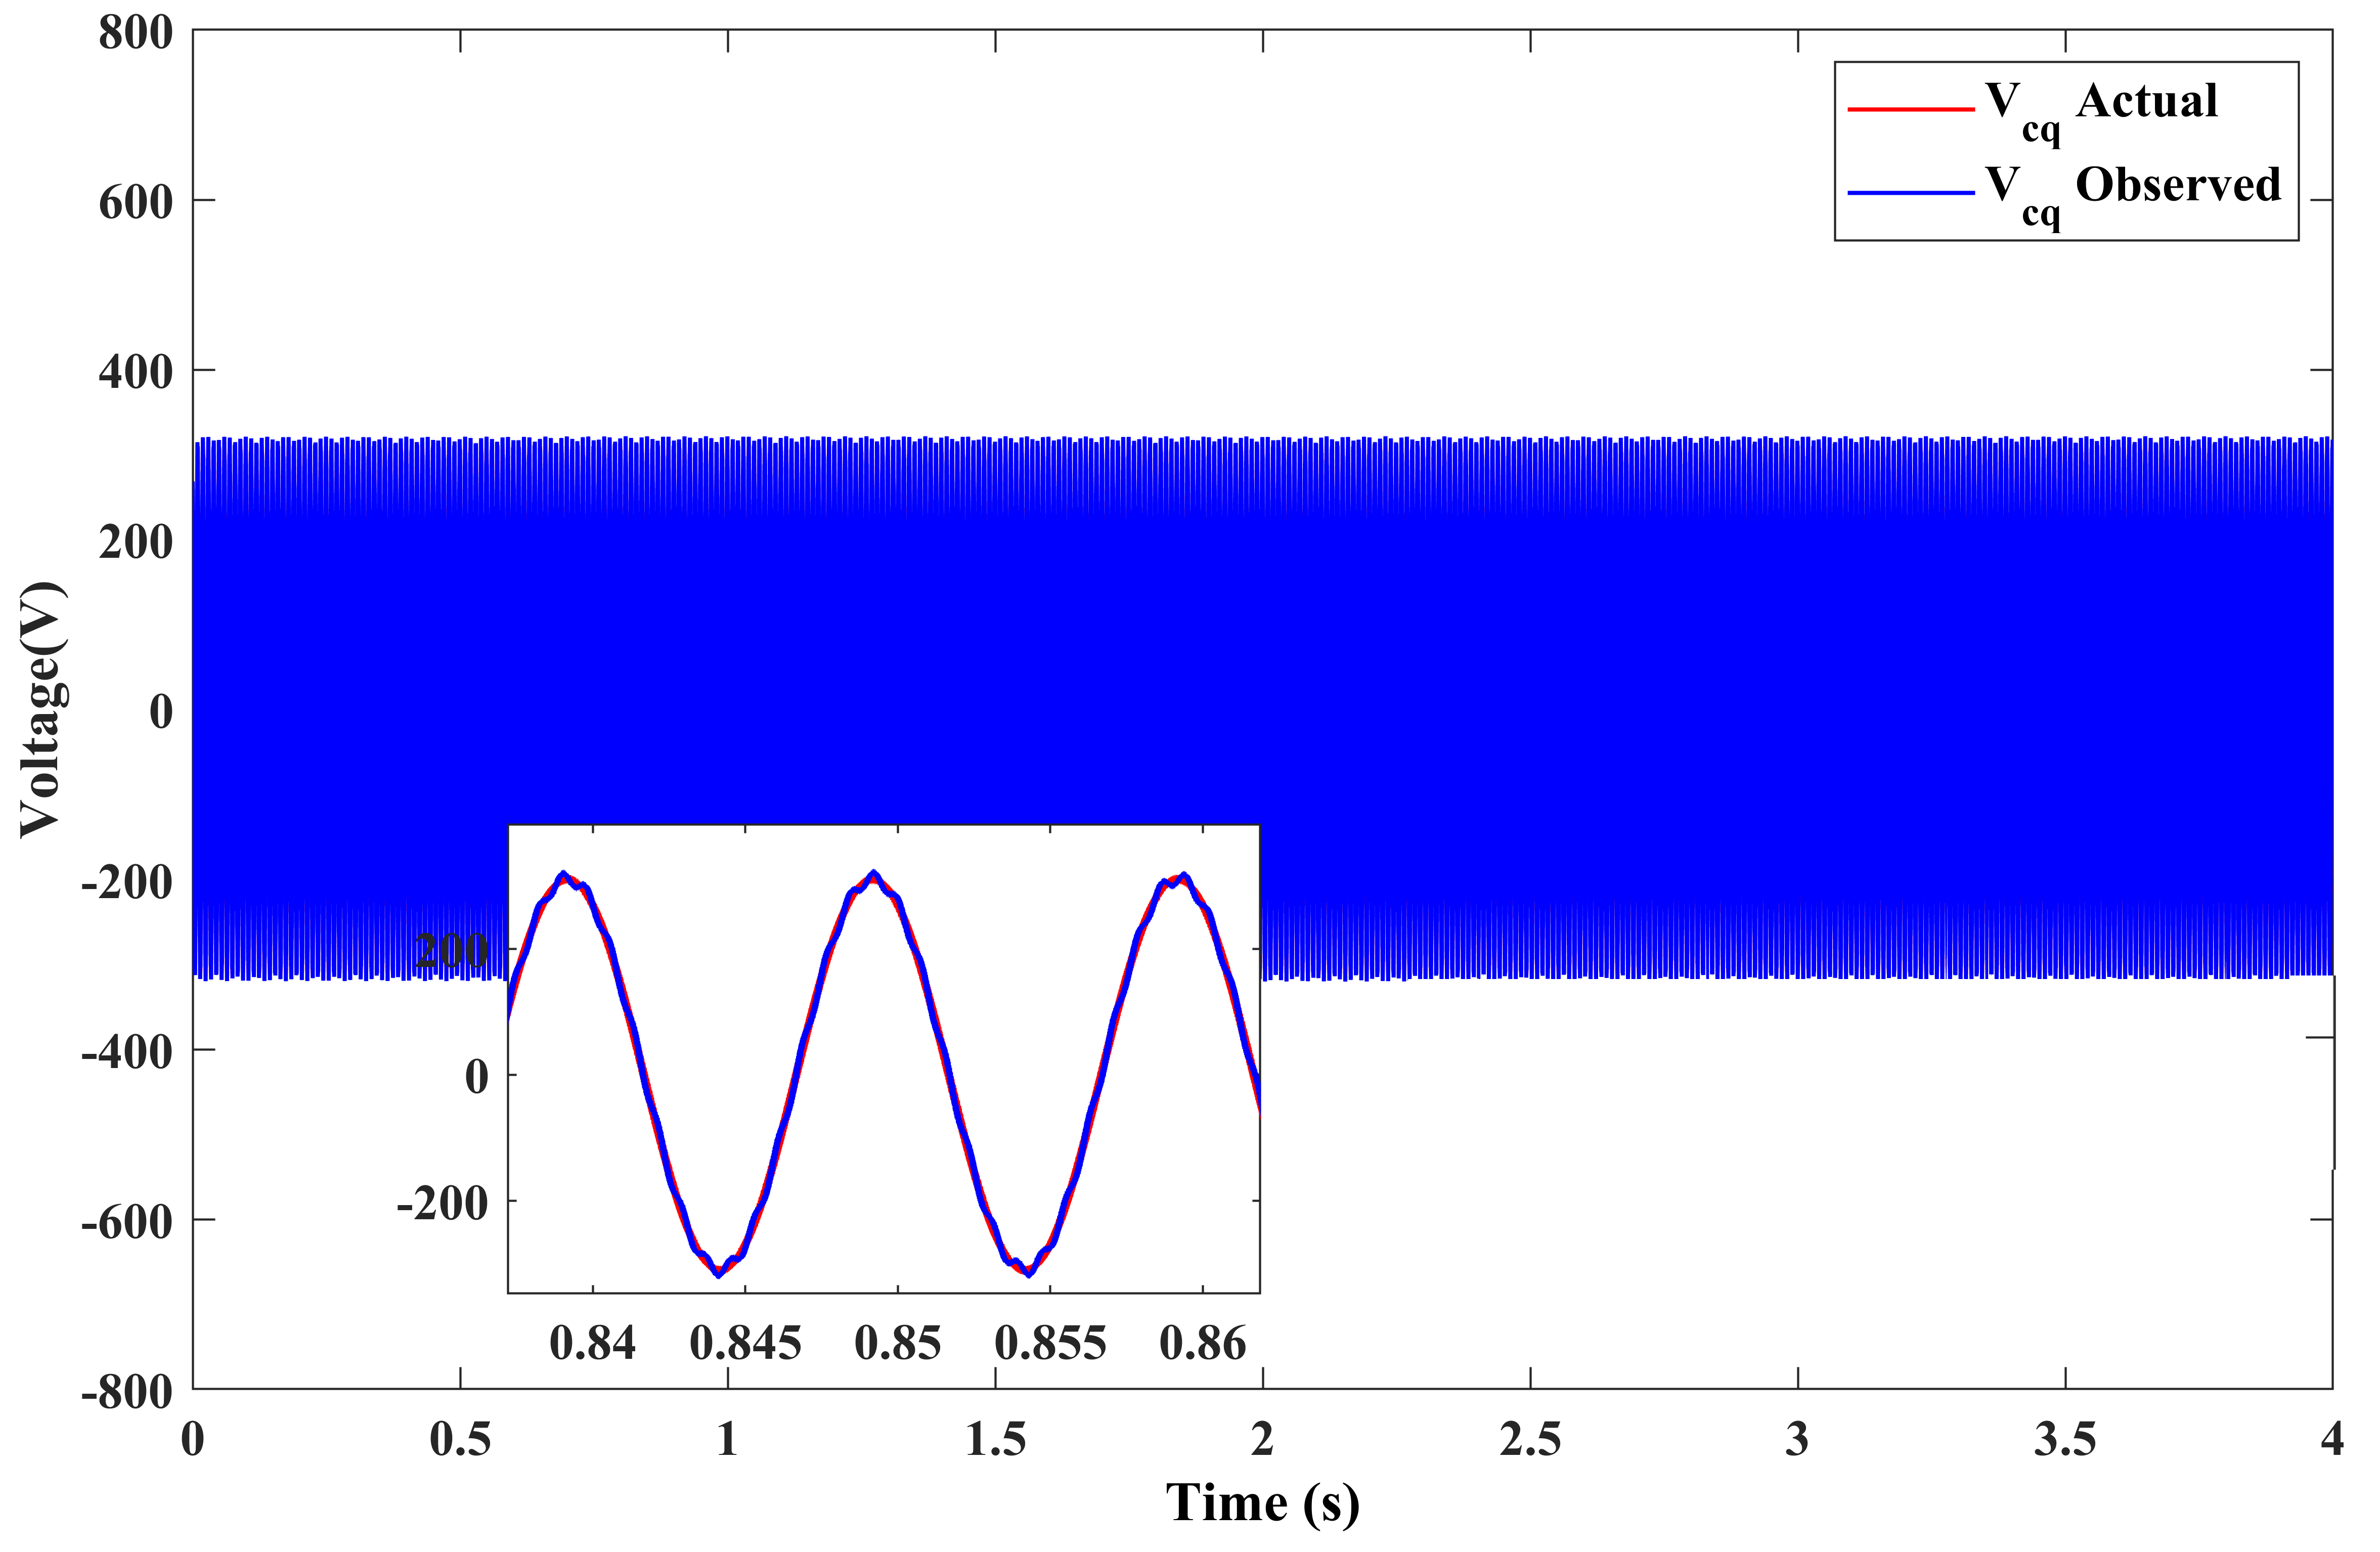
\includegraphics[width=\textwidth, height=4cm]{Pictures/Vcq Observed new1.png}
        \caption{Capacitor voltage $V_{cq}$: estimated vs. actual}
    \end{subfigure}

    % Third row of images
    \begin{subfigure}{0.45\textwidth}
        \centering
        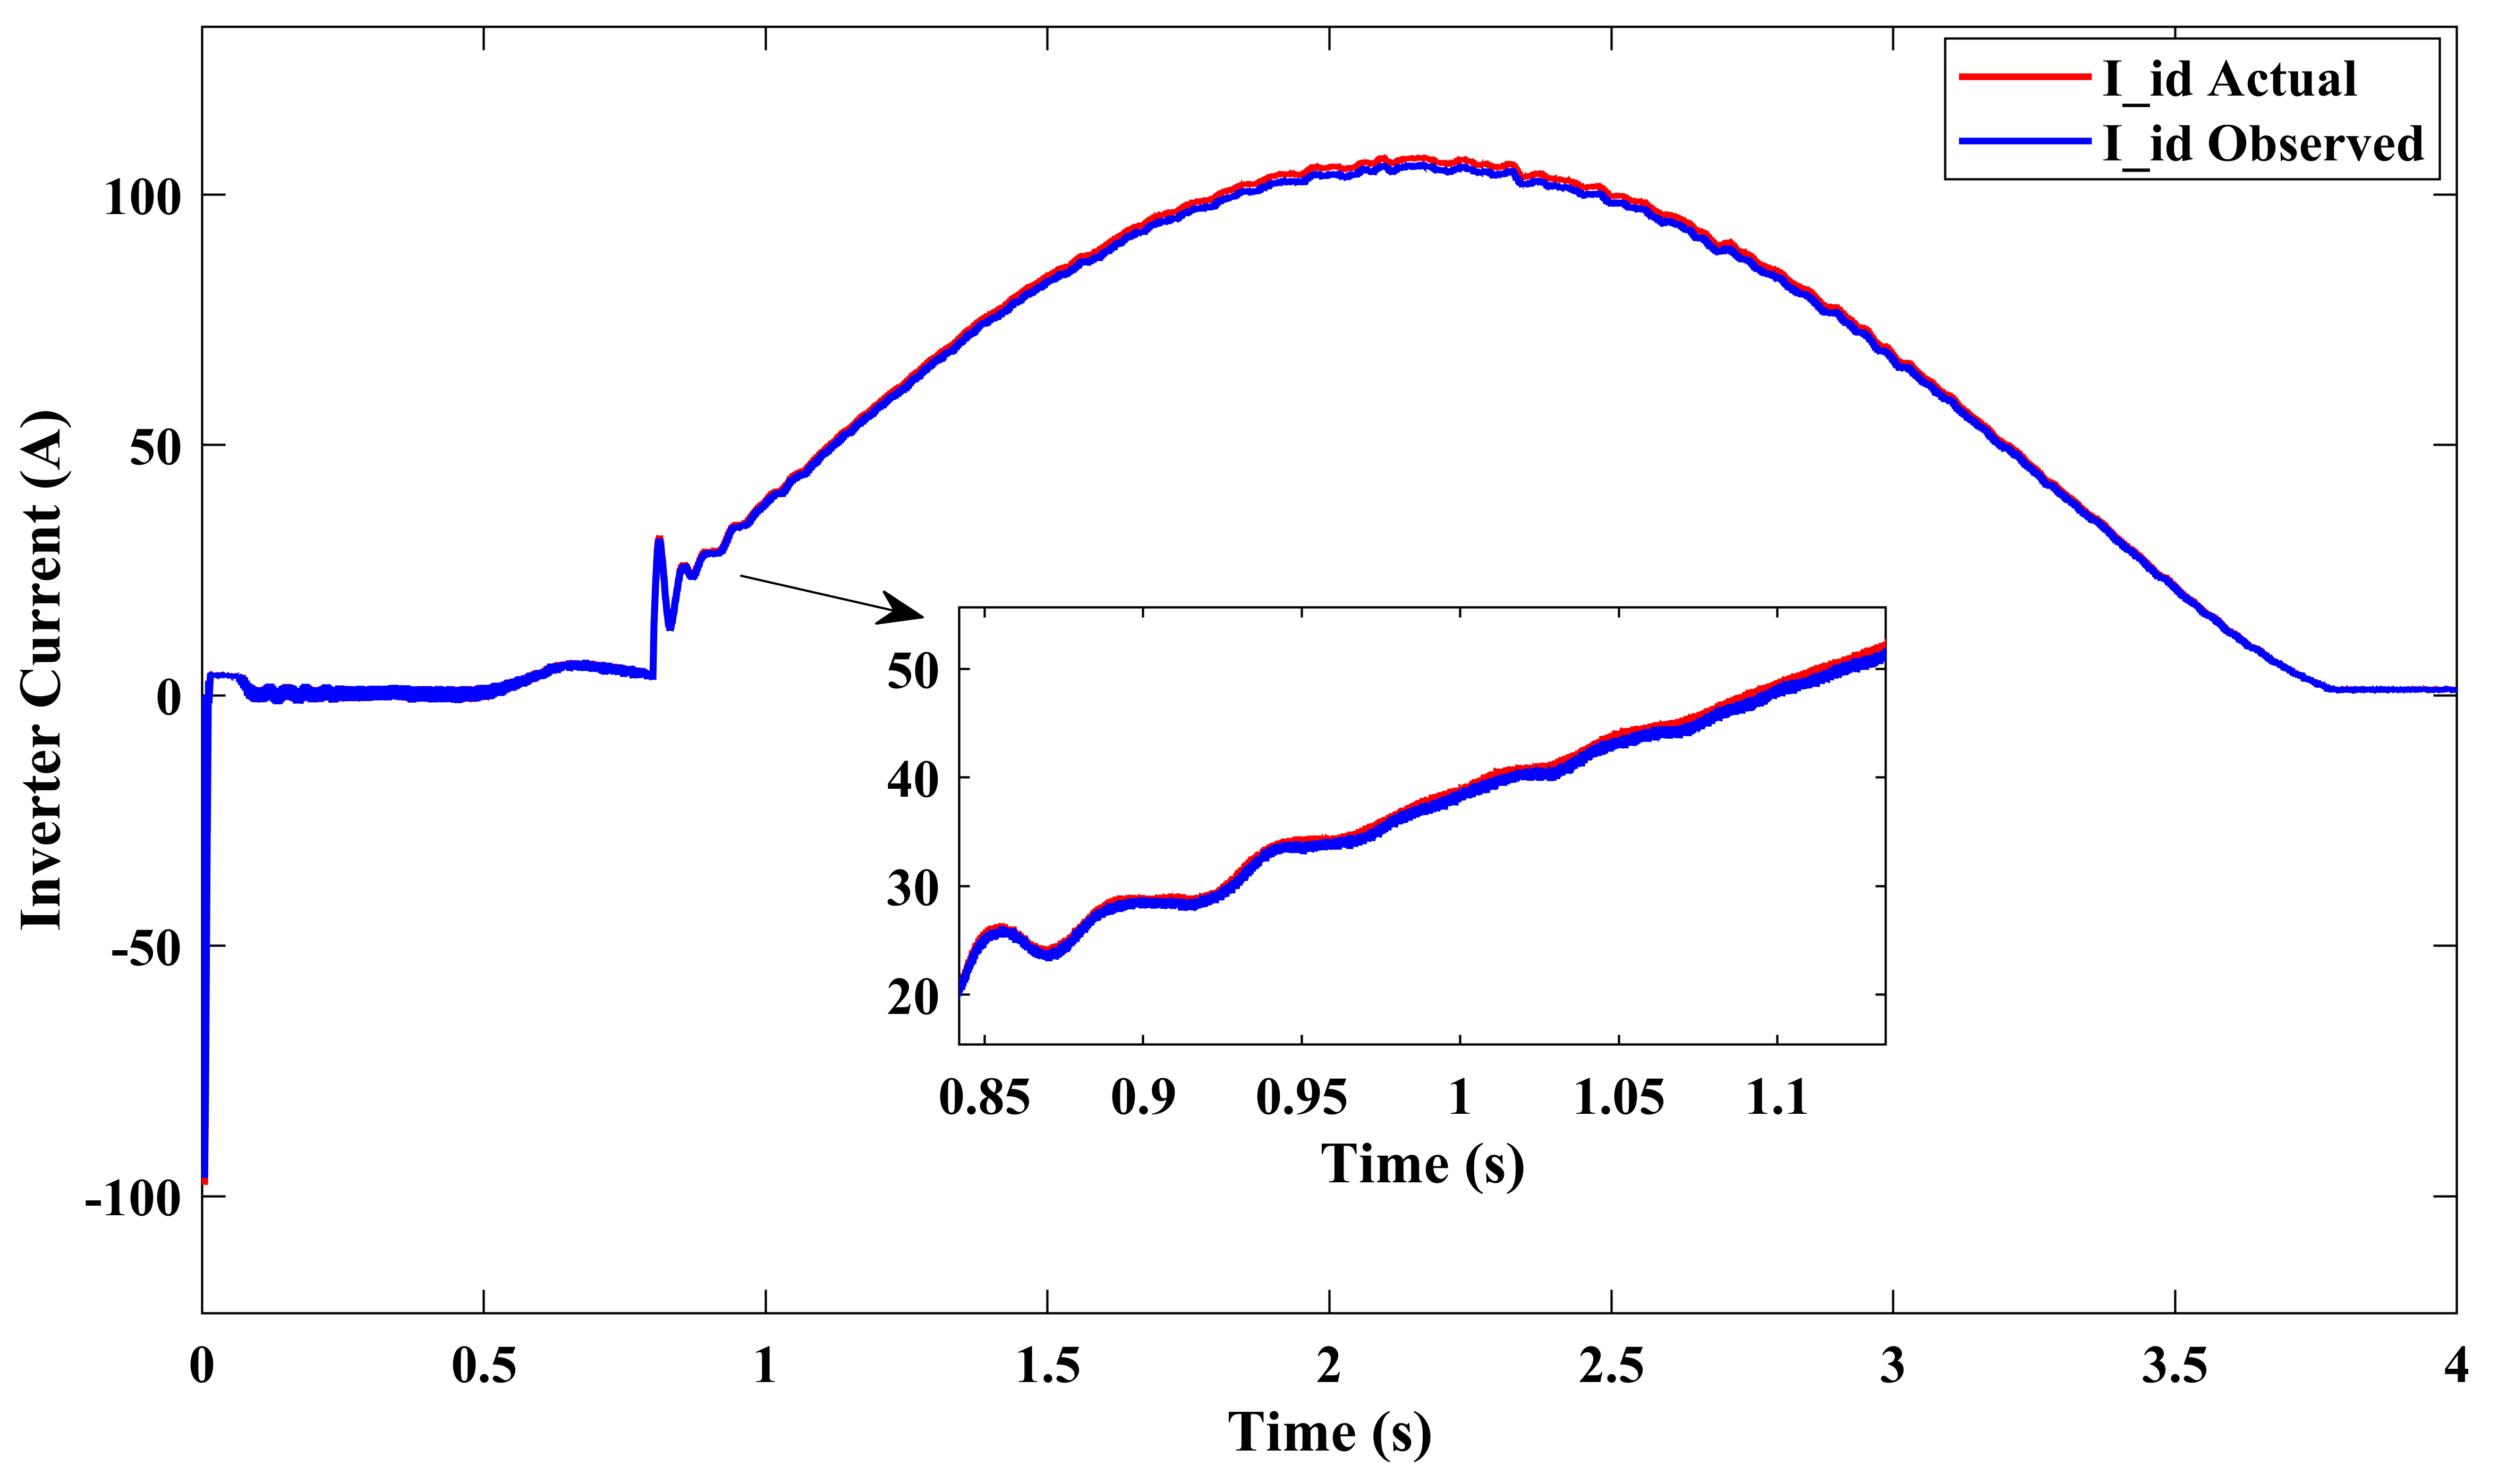
\includegraphics[width=\textwidth, height=4cm]{Pictures/Iid Observated.png}
        \caption{Inverter current $I_{d}$: estimated vs. actual}
    \end{subfigure}
    \hfill
    \begin{subfigure}{0.45\textwidth}
        \centering
        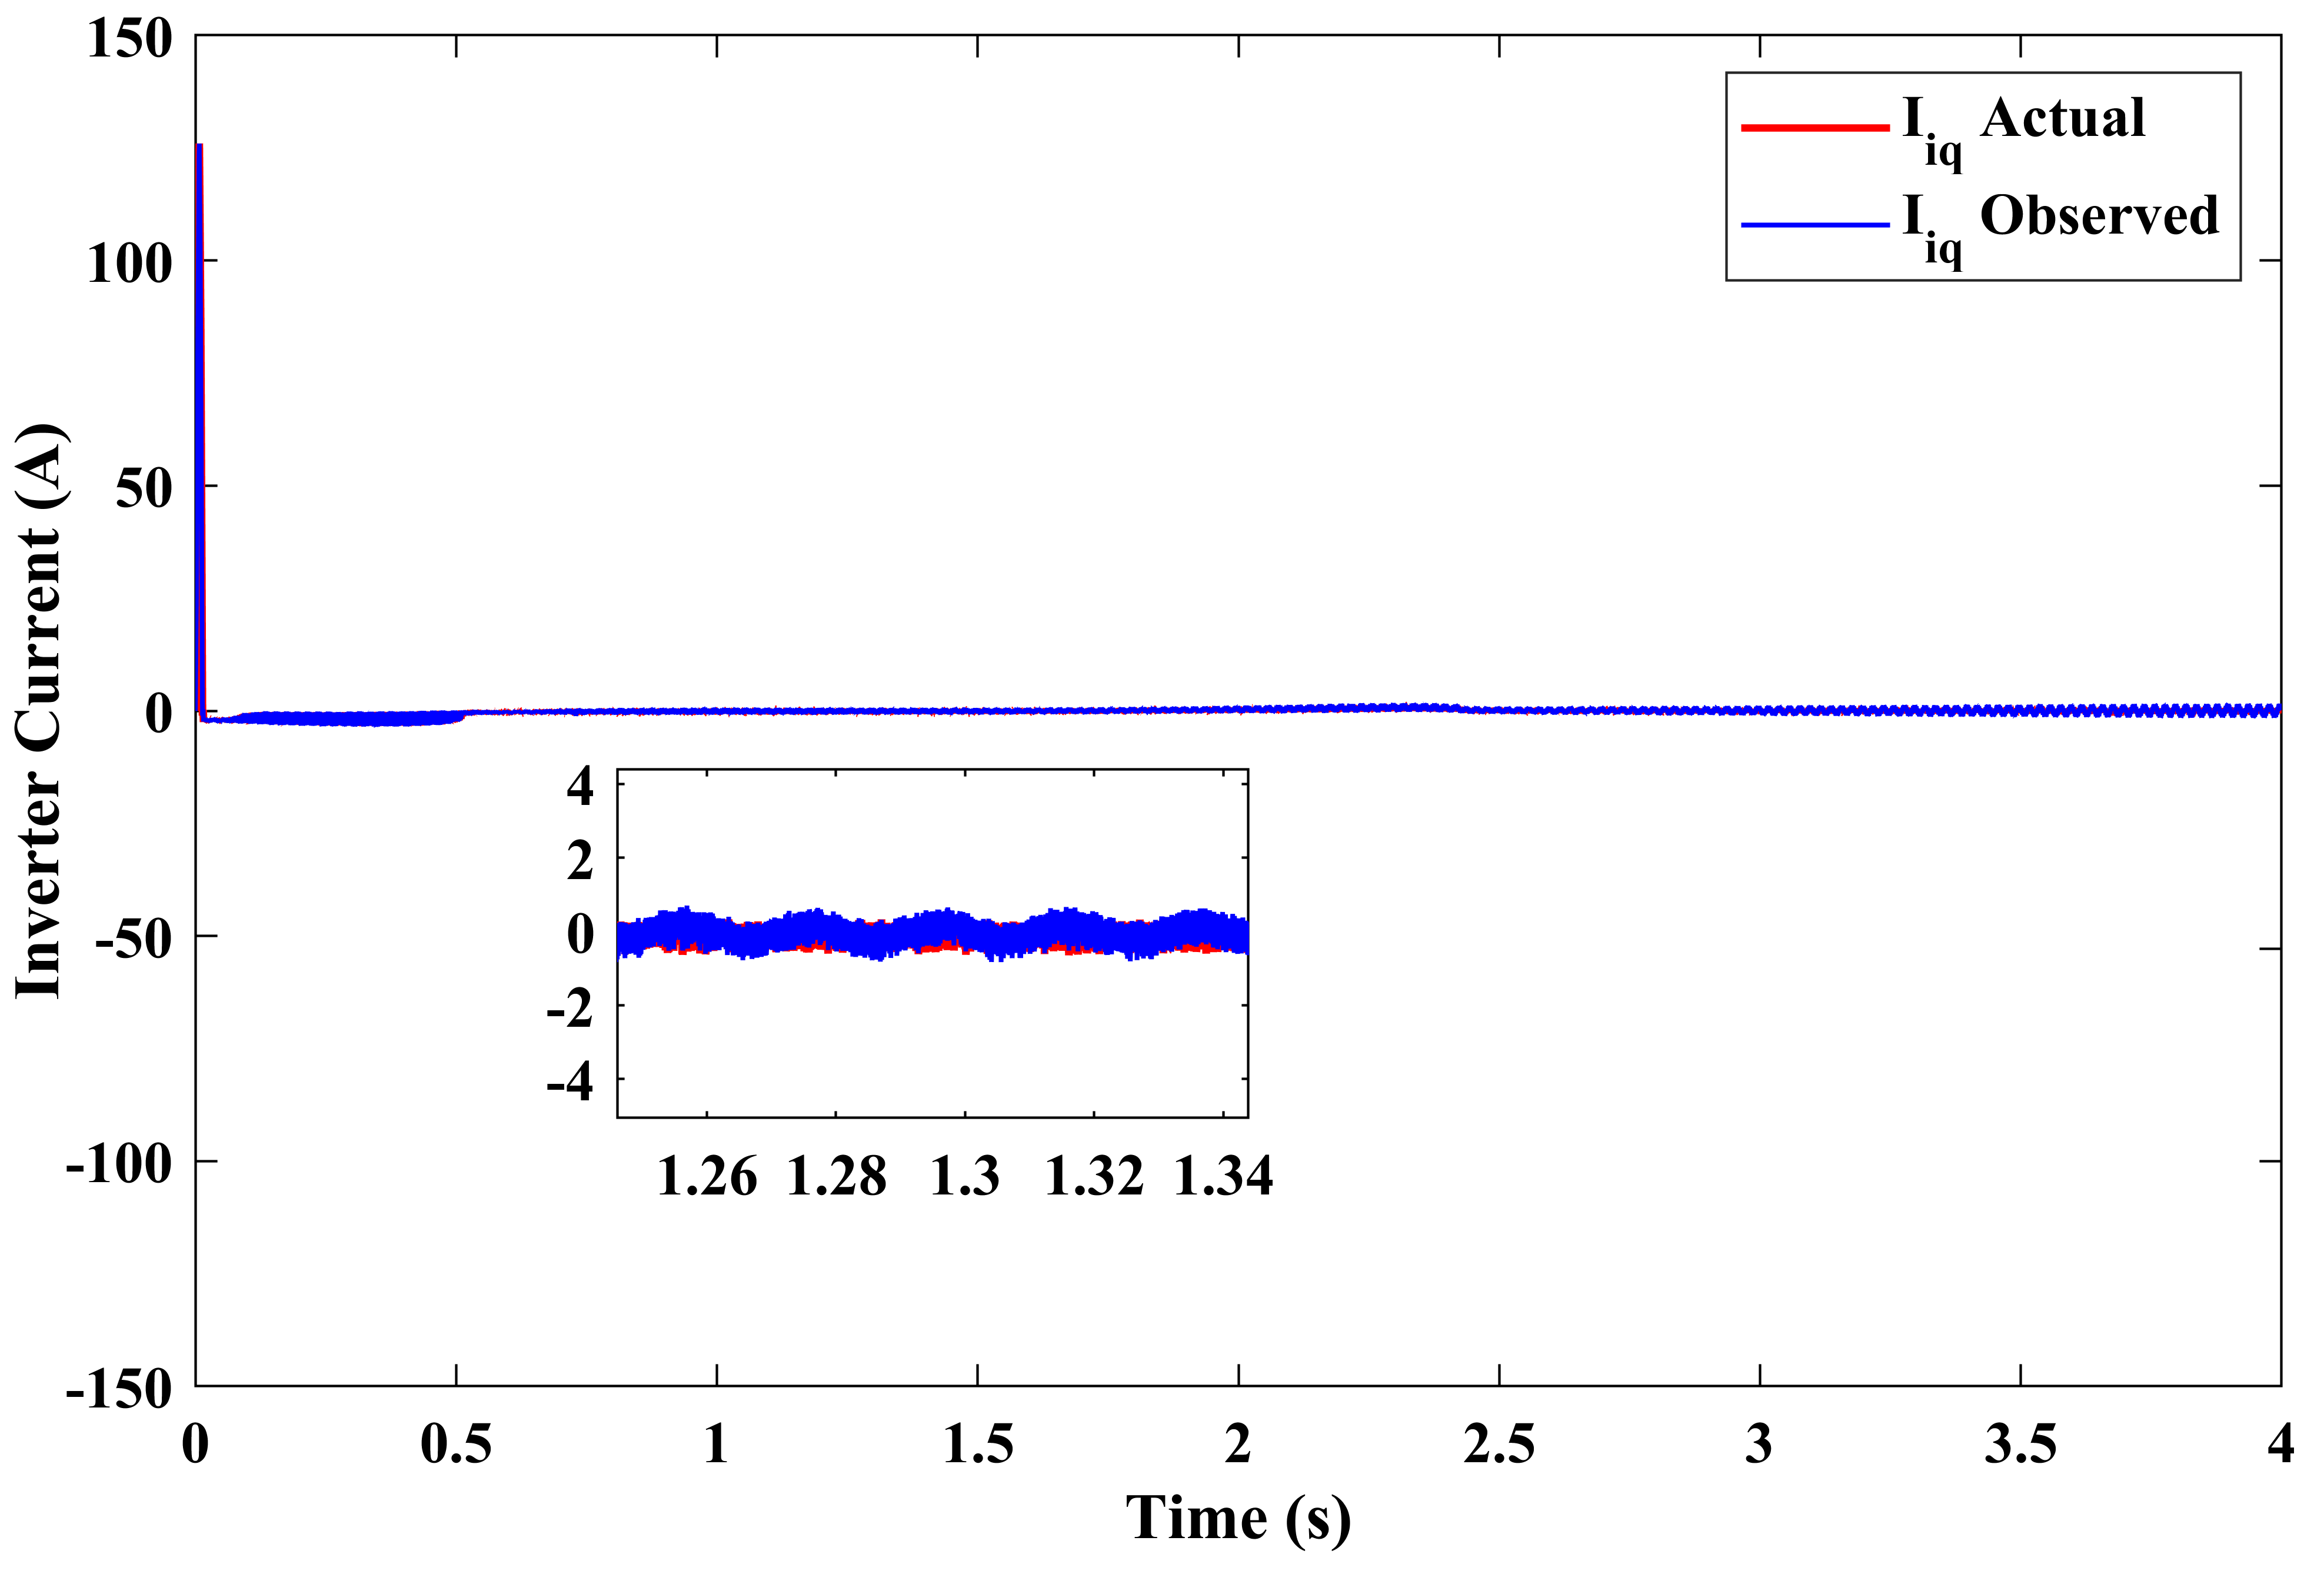
\includegraphics[width=\textwidth, height=4cm]{Pictures/Iiq Observed.png}
        \caption{Inverter current $I_{q}$: estimated vs. actual}
    \end{subfigure}
    
    \caption{Comparison of estimated and actual values of grid current, capacitor voltage and inverter current.}
    \label{fig:observer-results}
\end{figure}    

  
\subsection{Continuous Twisting Algorithm Controller Results}
The CTA controller was implemented on both the DC-DC converter (for MPPT tracking) and DC-AC inverter (for power quality regulation). Compared with the traditional PI and VO-MPPT methods, the proposed scheme achieves superior tracking accuracy, rapid response to irradiance variations, and minimal voltage/current fluctuations, thereby maximizing power extraction from the PV array.
\subsubsection{MPPT Tracking Performance}
The CTA controller dynamically adjusts the PV voltage and current to track irradiance fluctuations, ensuring precise reference power tracking (Fig. ~\ref{fig:cta-mppt-results}). The grid current variations aligned with the irradiance changes, demonstrating the ability of the controller to maintain optimal power extraction under transient conditions.
\begin{figure}
    \centering
    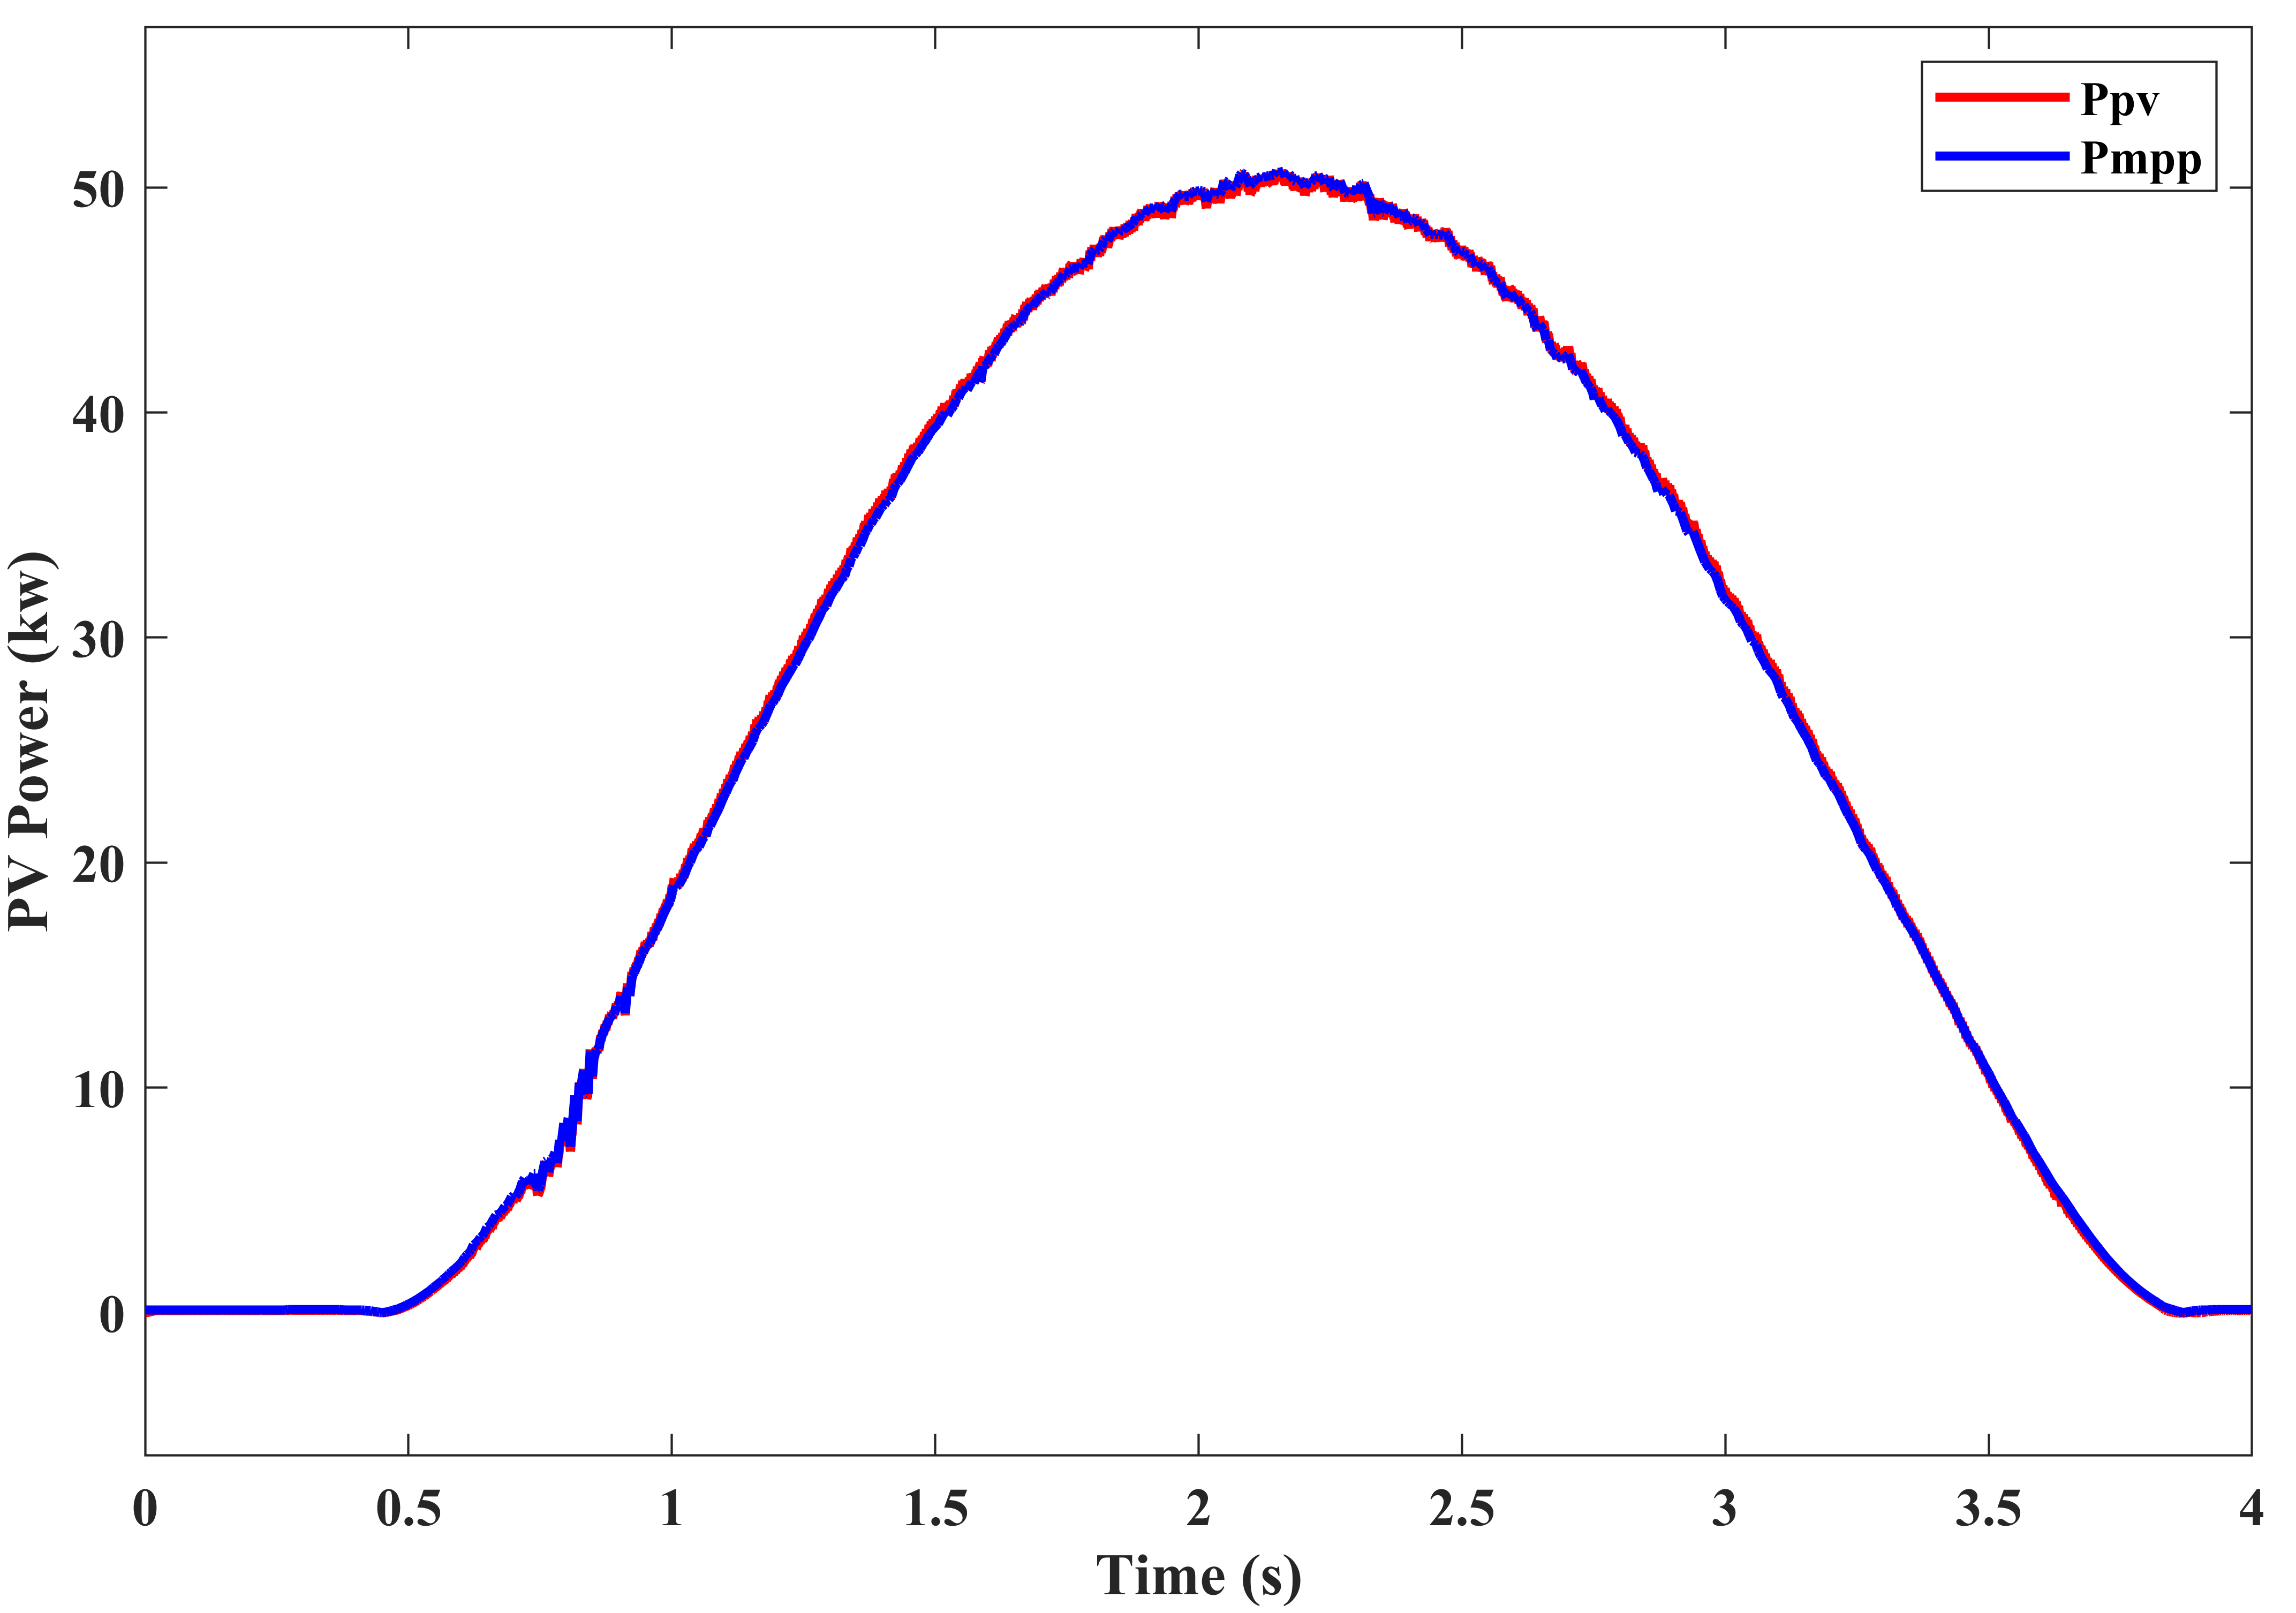
\includegraphics[width=\linewidth]{Pictures/CTA_MPPT.png}
    \caption{PV power and MPPT tracking under CTA controller}
    \label{fig:cta-mppt-results}
\end{figure}

\subsection{Inverter or Grid-Side Controller Performance}
The CTA-SMC controller achieves full active power injection into the grid (Fig. ~\ref{fig:cta-grid-power}), with the output power dynamically adjusted to the irradiance variation. The voltage and current oscillations were suppressed, thereby reducing harmonic distortion. As shown in Fig.~\ref{fig:grid-current-thd}, the grid current’s Total Harmonic Distortion (THD) is 0.43\%—well below the IEEE standard limit of 5\%—validating compliance with power quality norms.

\begin{figure}
    \centering
    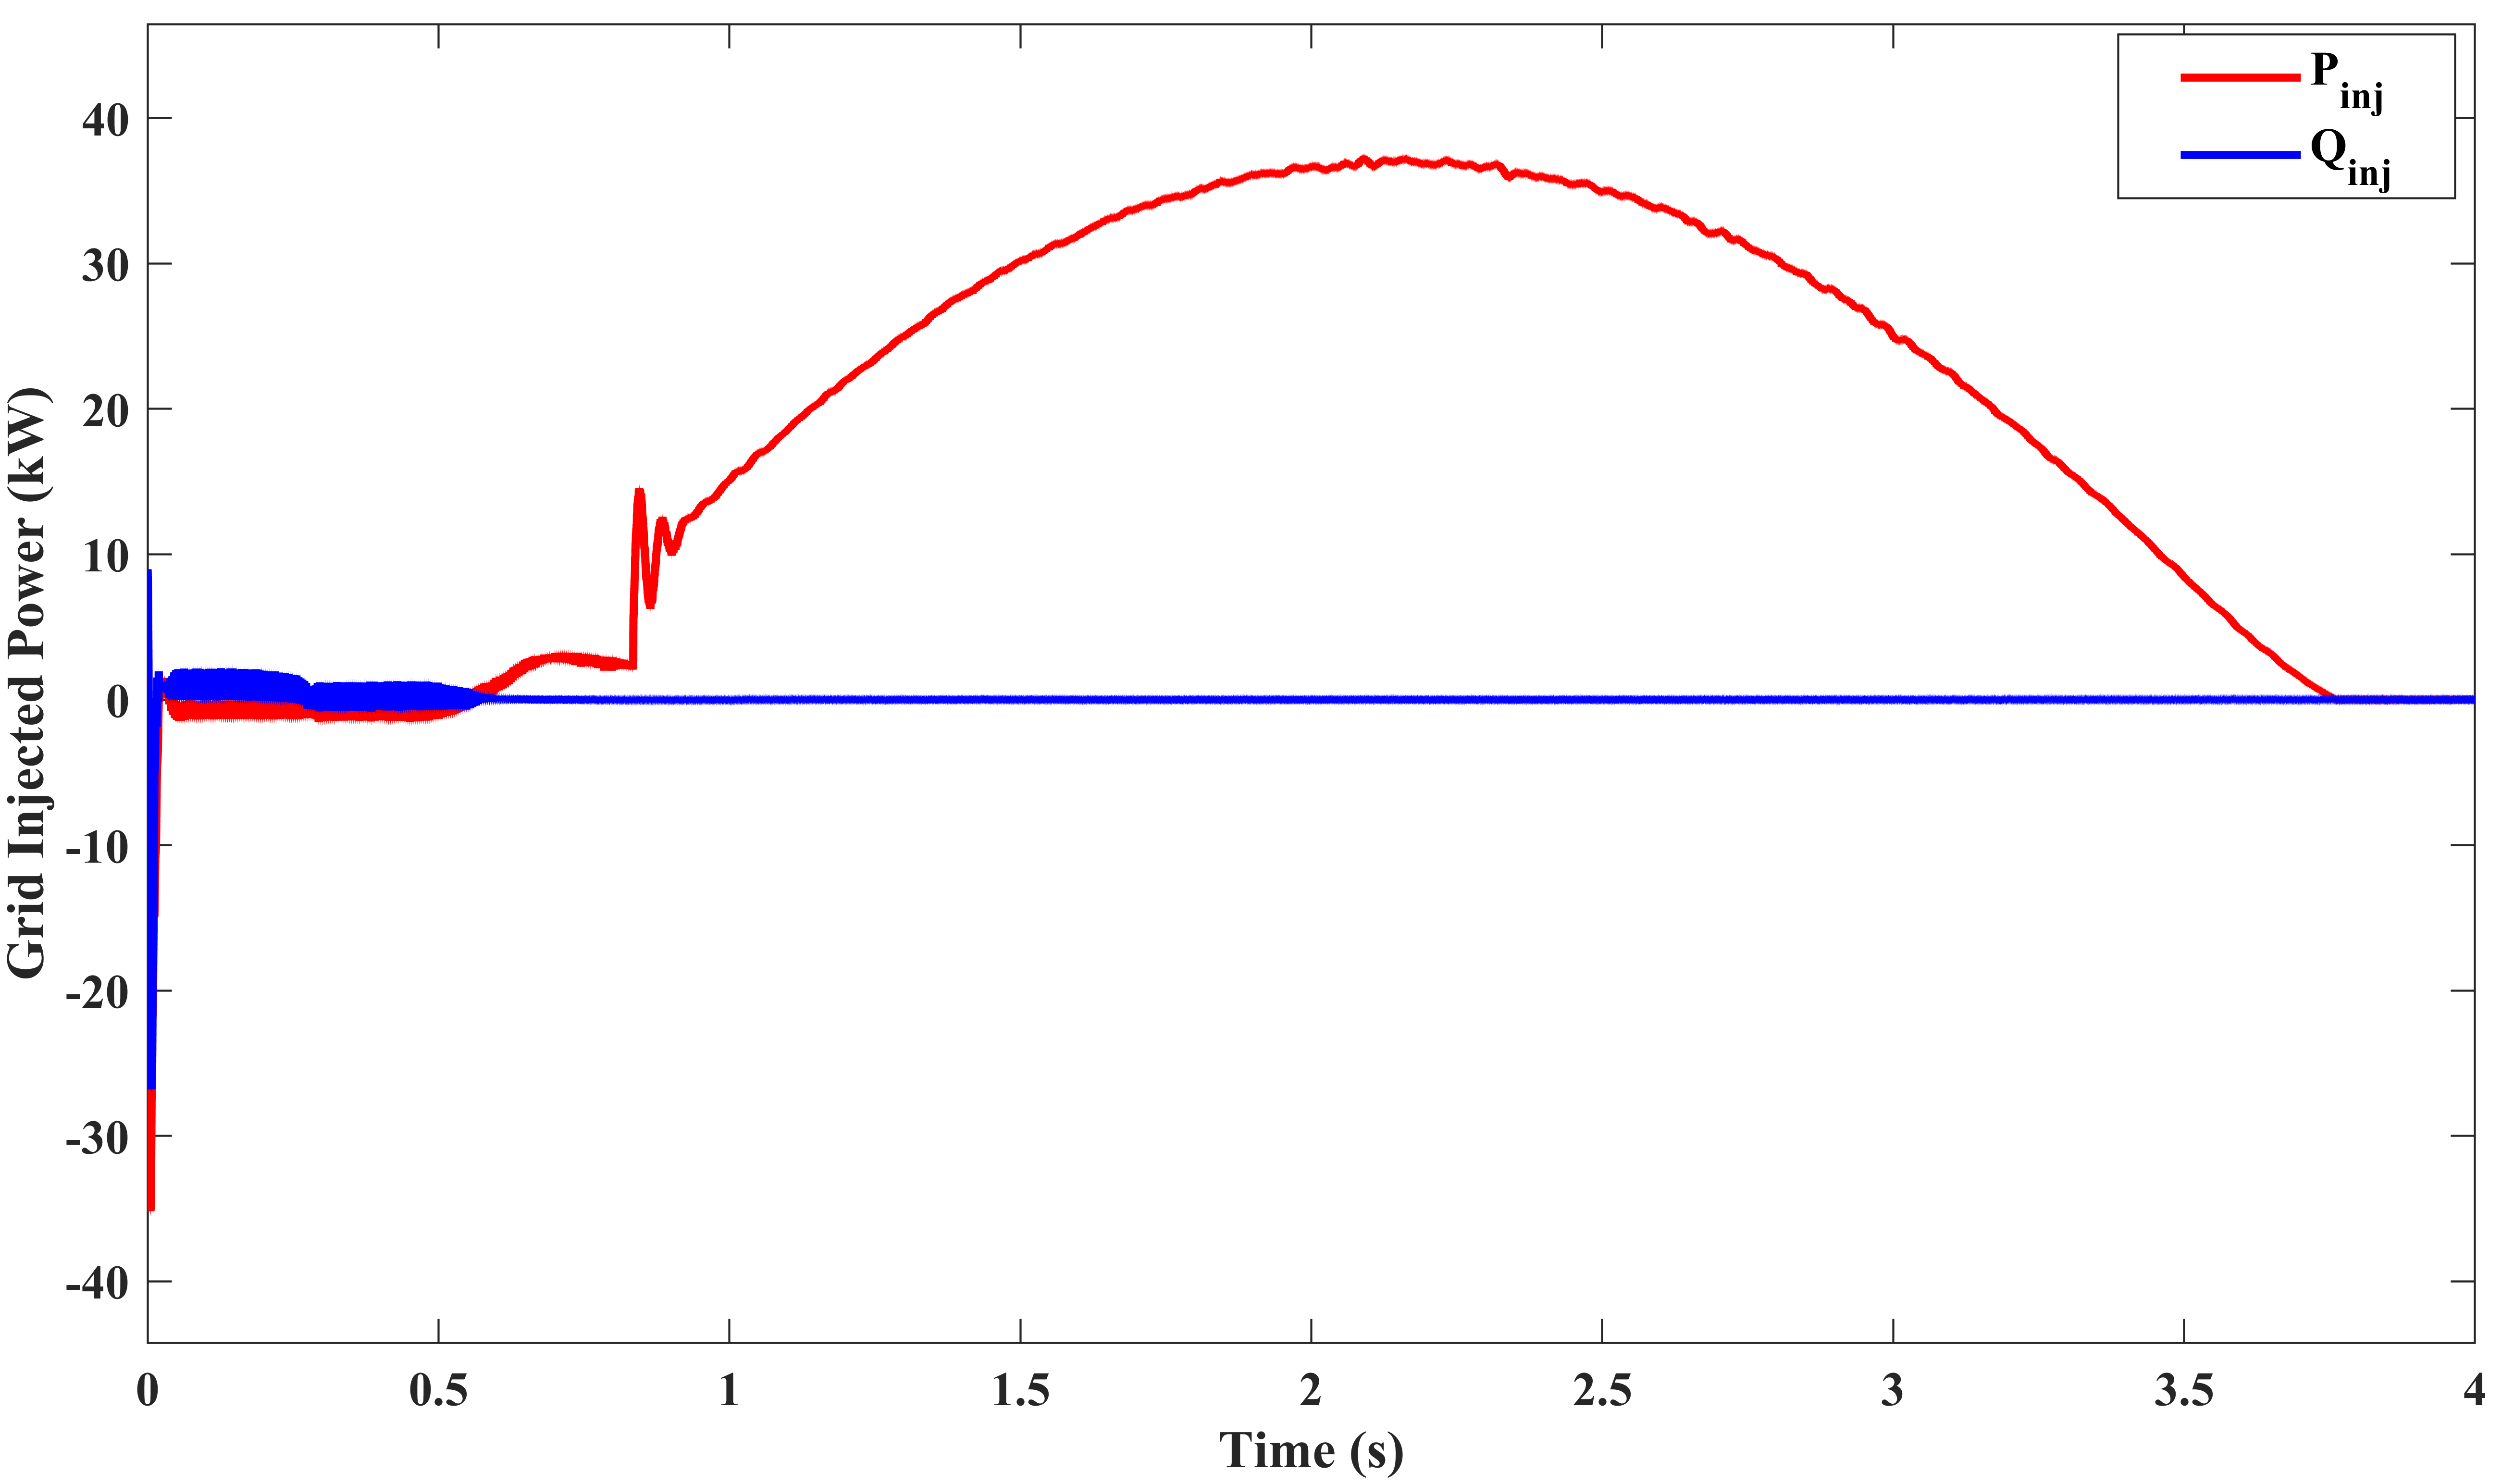
\includegraphics[width=\linewidth]{Pictures/CTA Power injected.png}
    \caption{Active power injected into the grid under CTA control}
    \label{fig:cta-grid-power}
\end{figure}

Fast Fourier Transform (FFT) analysis confirmed the effectiveness of the CTA controller in mitigating harmonics, ensuring robust performance in systems requiring strict THD control. Additionally, the grid voltage and current remained perfectly synchronized (Fig. ~\ref{fig:grid-current-thd}(a)), achieving a unity power factor and maximizing real power delivery to the grid.

\begin{figure}[htbp]
    \centering
    % First row of images
    \begin{subfigure}{0.45\textwidth}
        \centering
        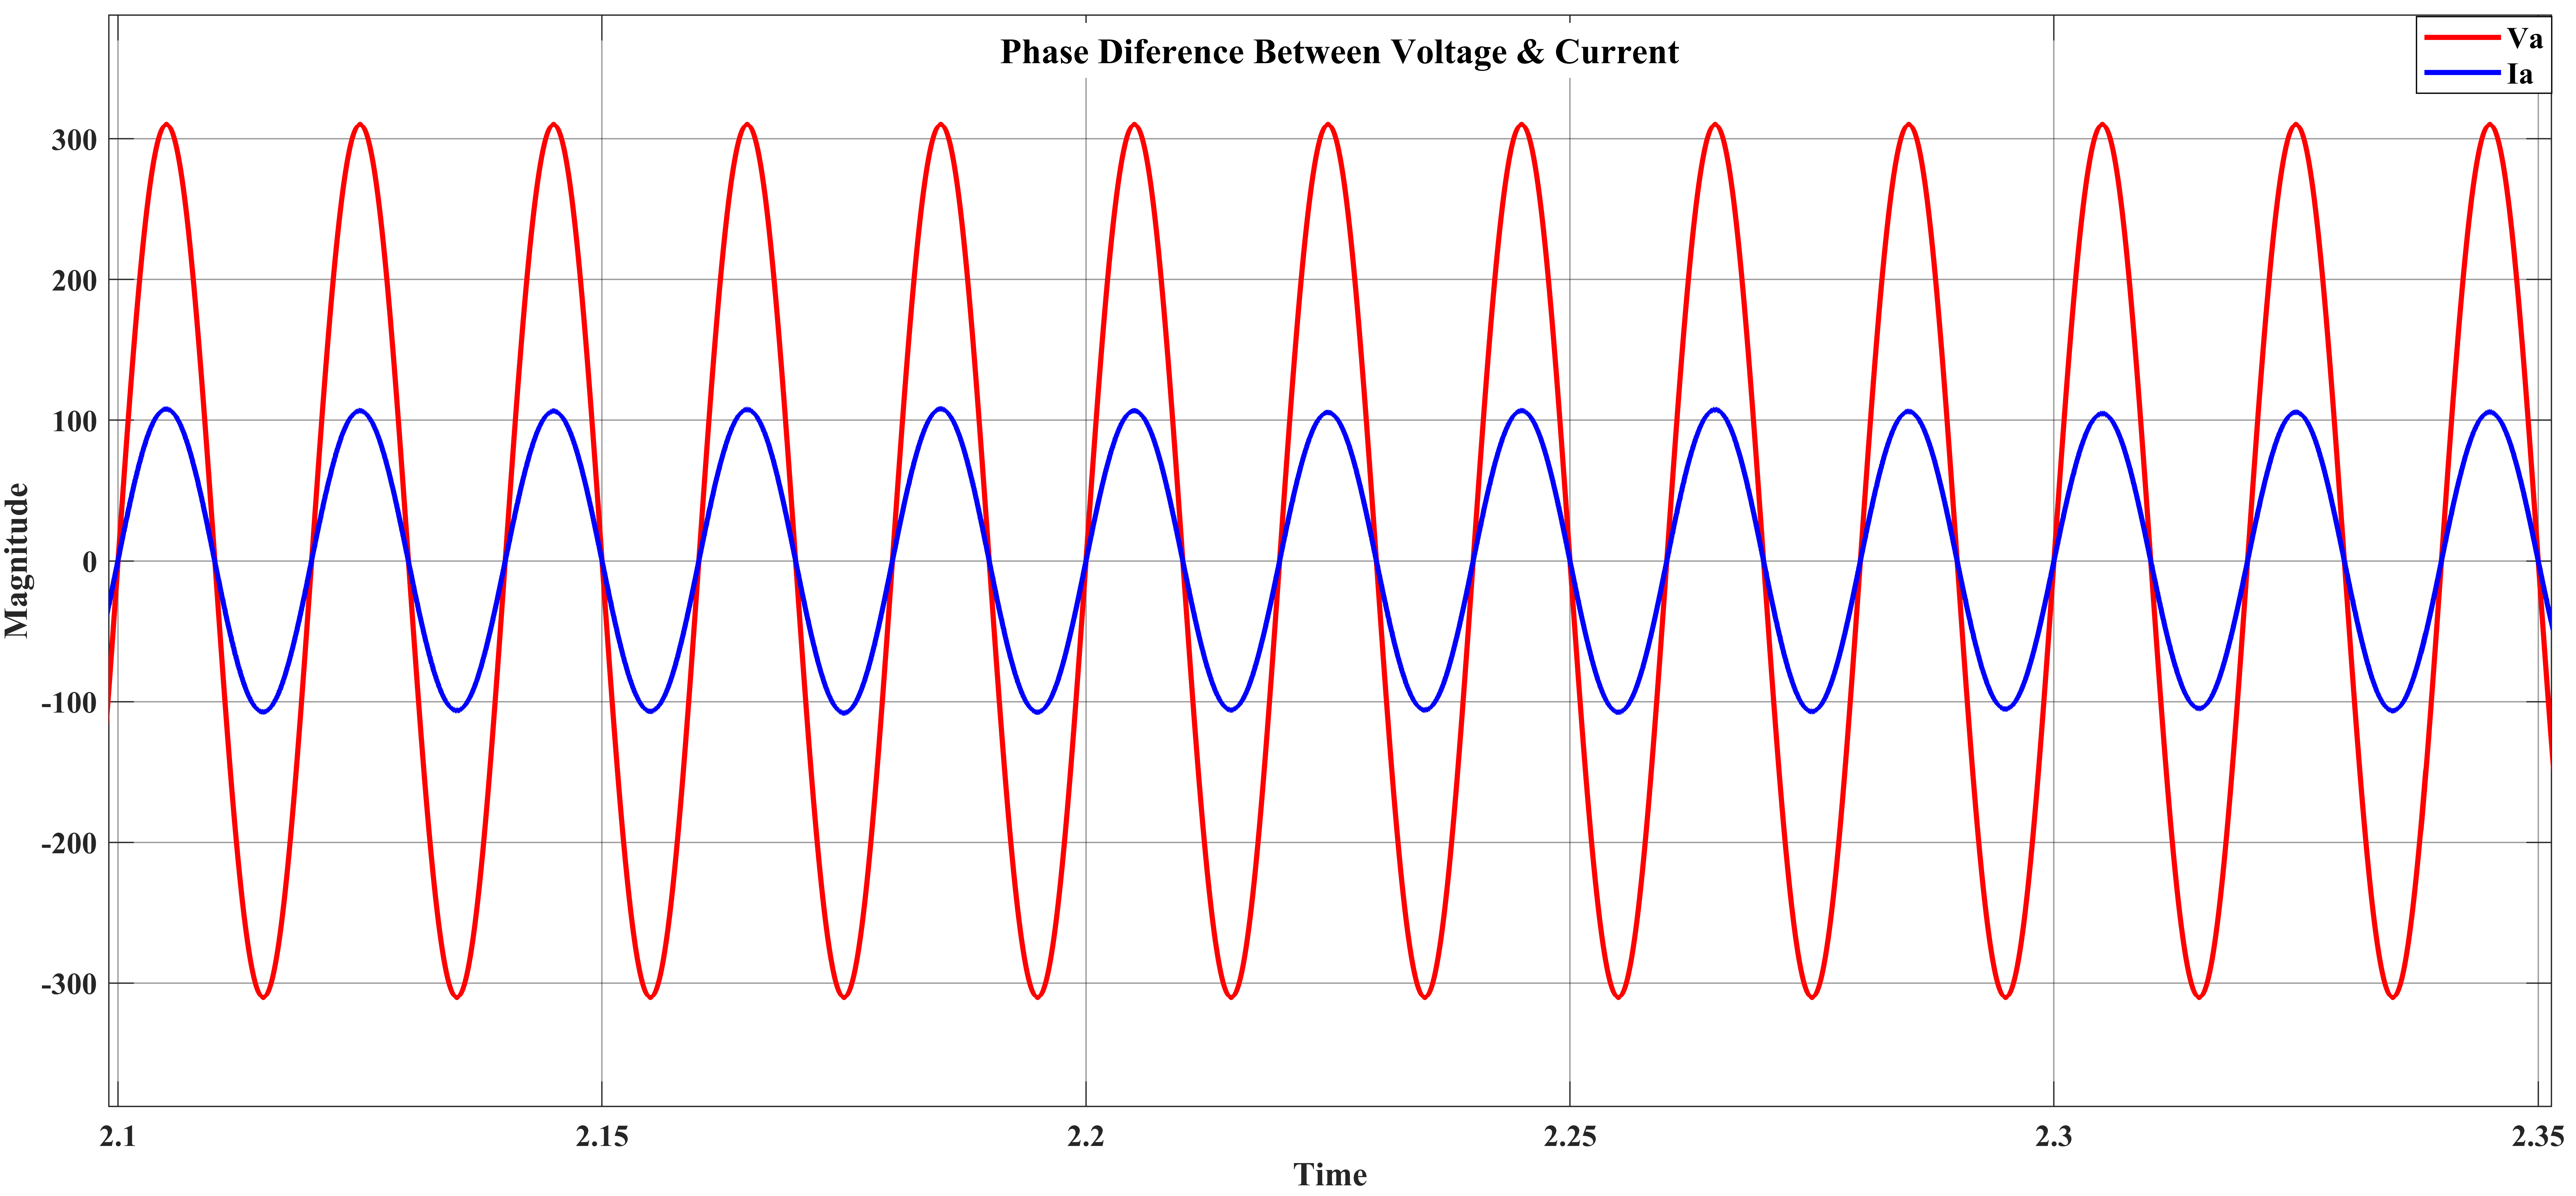
\includegraphics[width=\textwidth, height=4cm]{Pictures/CTA_SMC Phase Diference between V & I.png}
        \caption{Grid voltage-current phase synchronization under CTA control}
    \end{subfigure}
    \hfill
    \begin{subfigure}{0.45\textwidth}
        \centering
        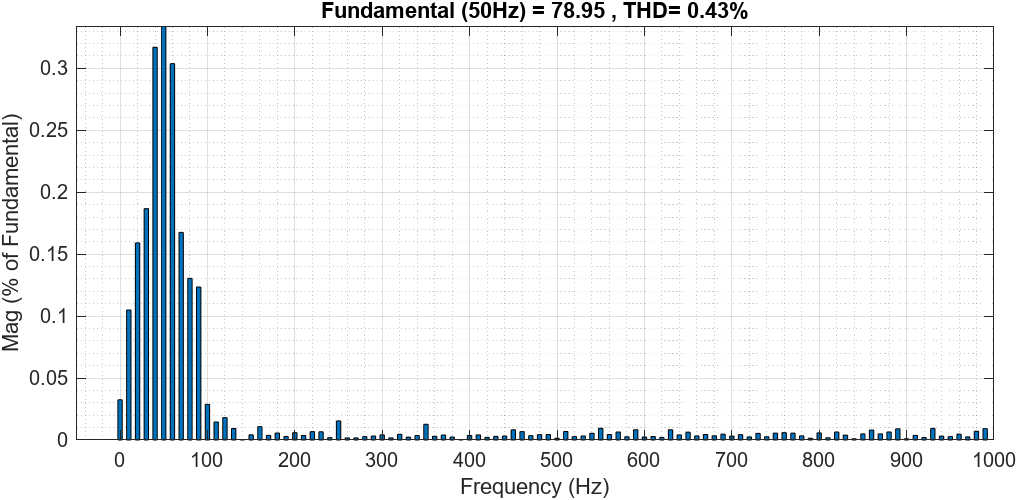
\includegraphics[width=\textwidth, height=4cm]{Pictures/CTA_SMC THD 2.png}
        \caption{Grid current THD spectrum under CTA control}
        \label{fig:grid-current-thd}
    \end{subfigure}
    \caption{CTA grid voltage/current synchronization and current THD.}
\end{figure}

\subsection{Discontinuous Integral Controller (DIC) Performance}
The Discontinuous Integral Controller (DIC) offers simplicity and low computational complexity, making it ideal for dual-stage grid-connected PV systems. Implemented for both MPPT tracking and inverter control, the DIC enhances the power quality and system stability under dynamic operating conditions.

\subsubsection{MPPT Tracking Performance}
The DIC improves the MPPT efficiency by robustly rejecting disturbances caused by rapid fluctuations in irradiance or temperature (Fig. ~\ref{fig:dic-mppt-results}). Unlike conventional methods, its discontinuous integration of tracking errors ensures fast convergence to the maximum power point (MPP), minimizes deviations, and maximizes the energy yield under varying climatic conditions.

\begin{figure}
    \centering
    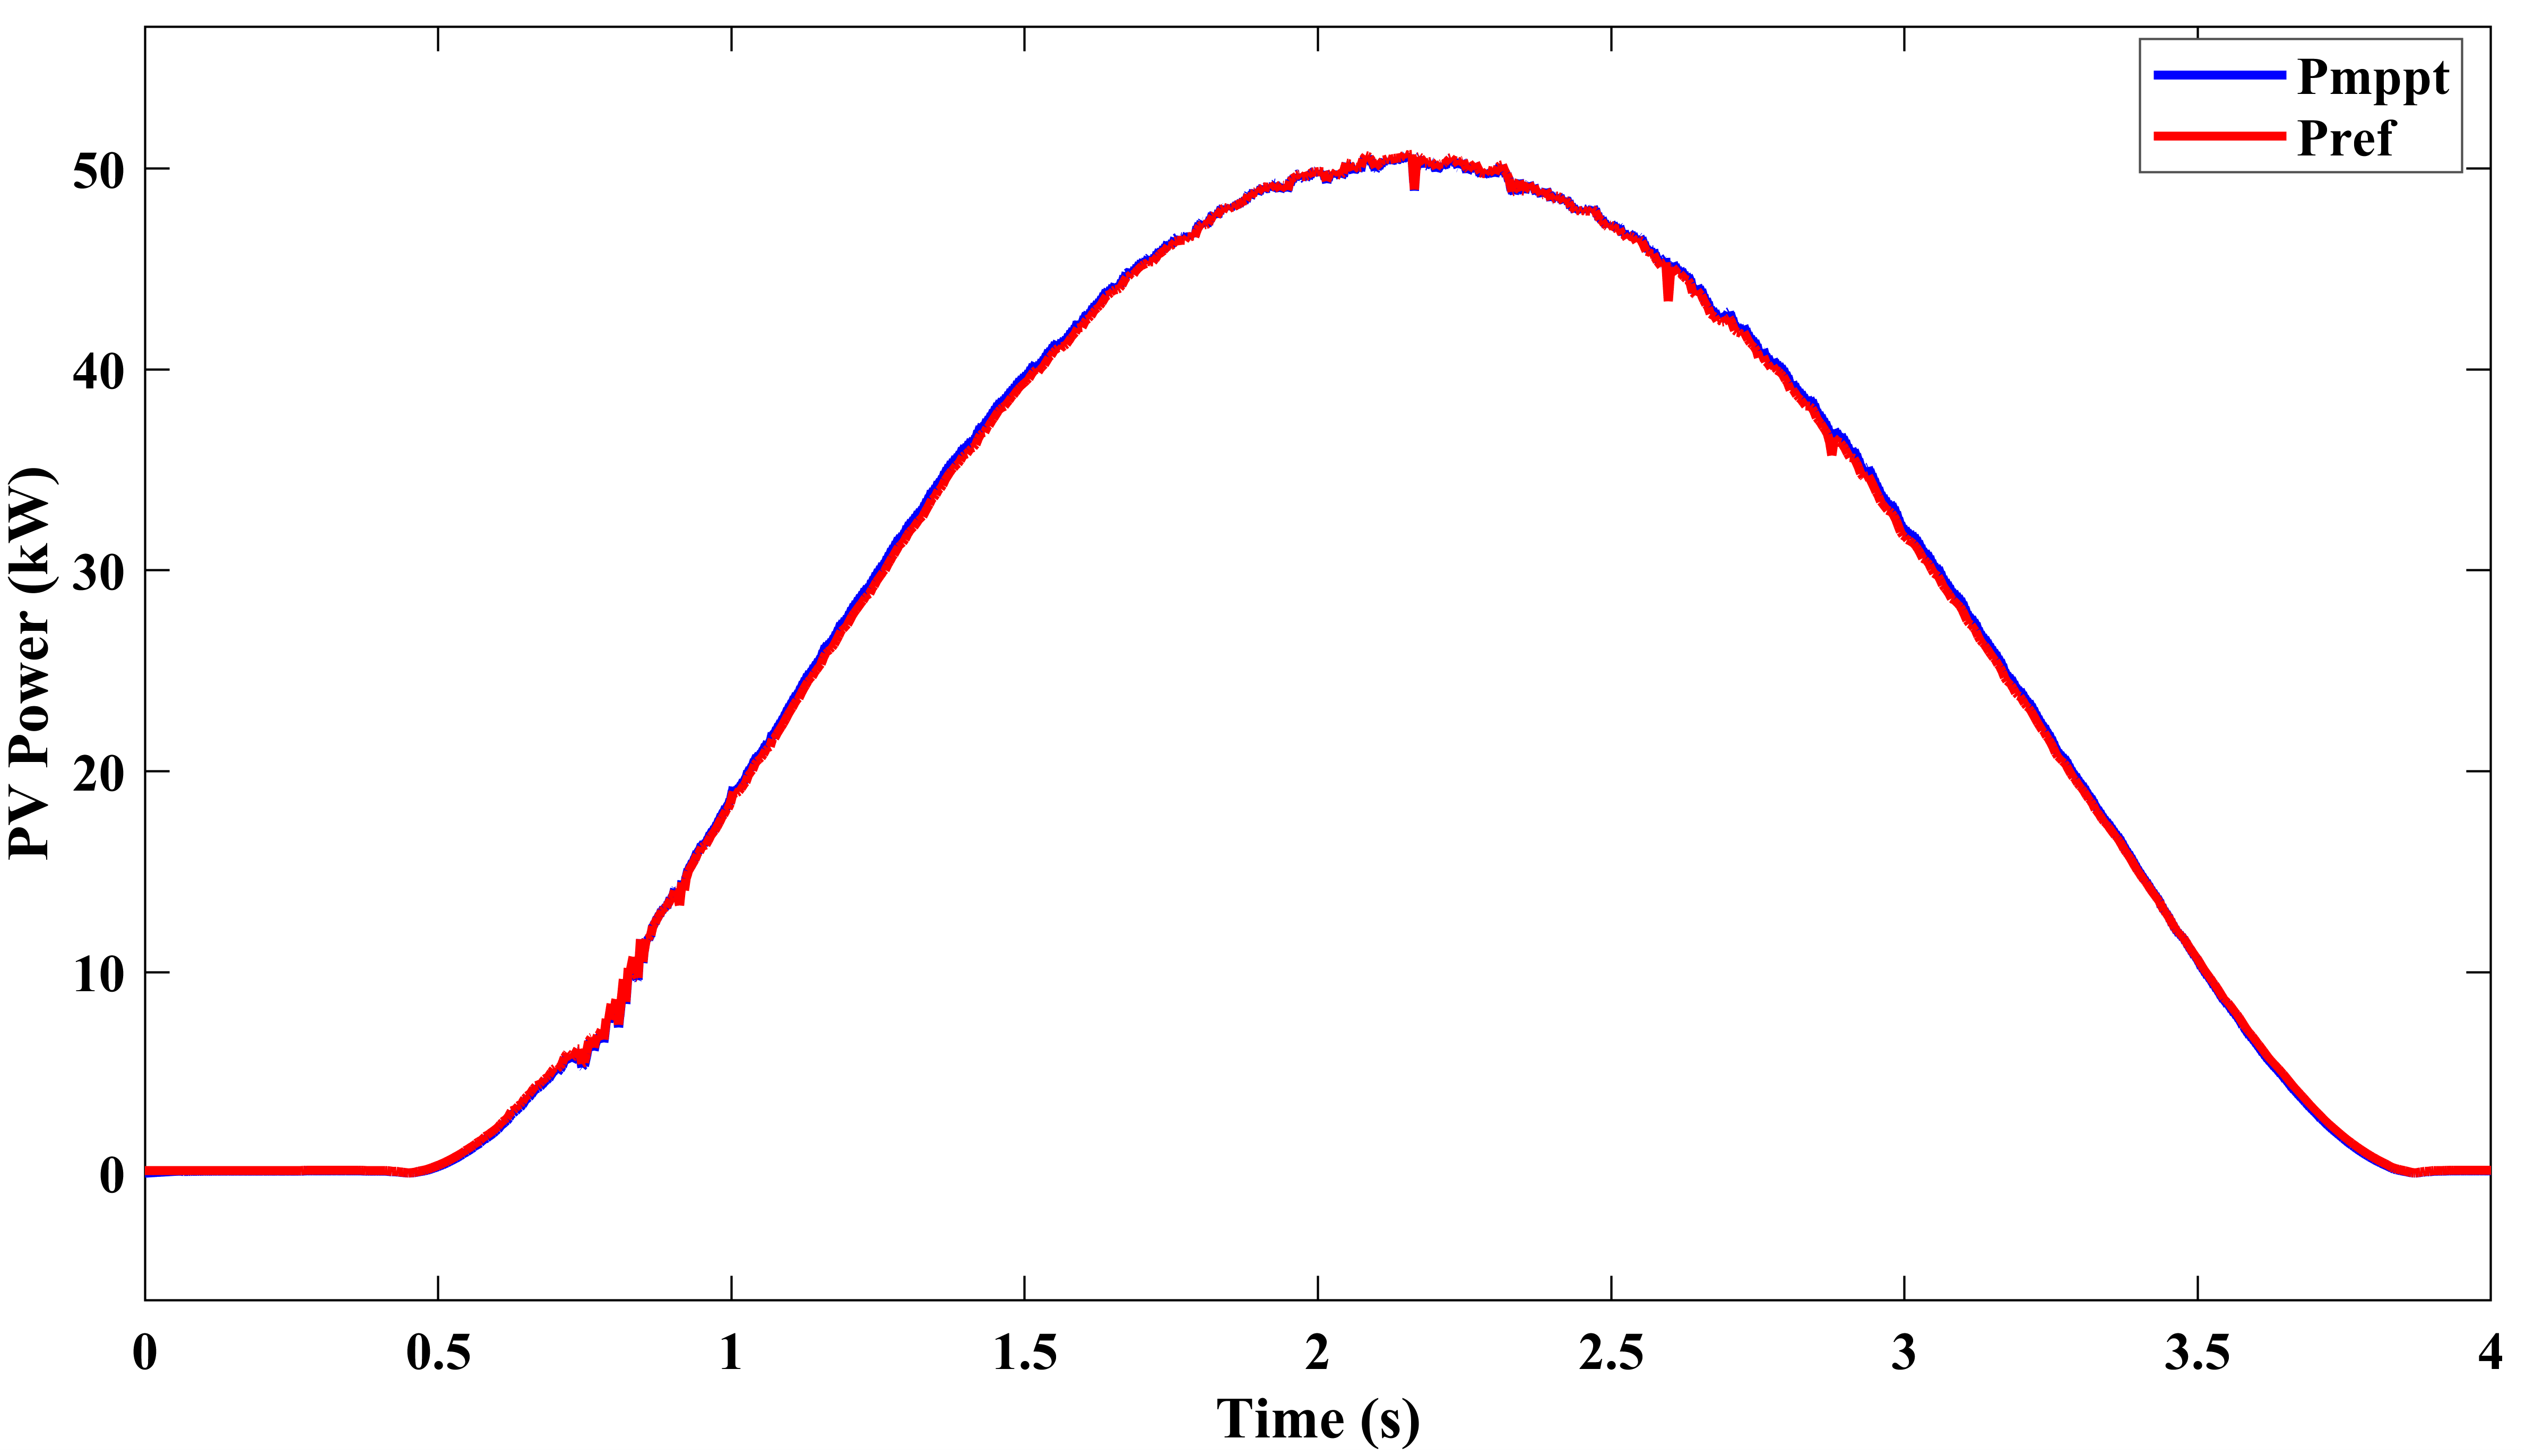
\includegraphics[width=\linewidth]{Pictures/DIC_MPPT.png}
    \caption{PV power and MPPT tracking under DIC controller}
    \label{fig:dic-mppt-results}
\end{figure}

\subsubsection{Inverter and Grid-Side Performance}
The DIC regulates the grid-side voltage and current, mitigating voltage sag, swell, and harmonic distortion. Its discontinuous integral action ensures rapid adaptation to grid disturbances while maintaining stable power injection and high power quality, as shown in Fig. ~\ref{fig:dic-grid-power}.

\begin{figure}
    \centering
    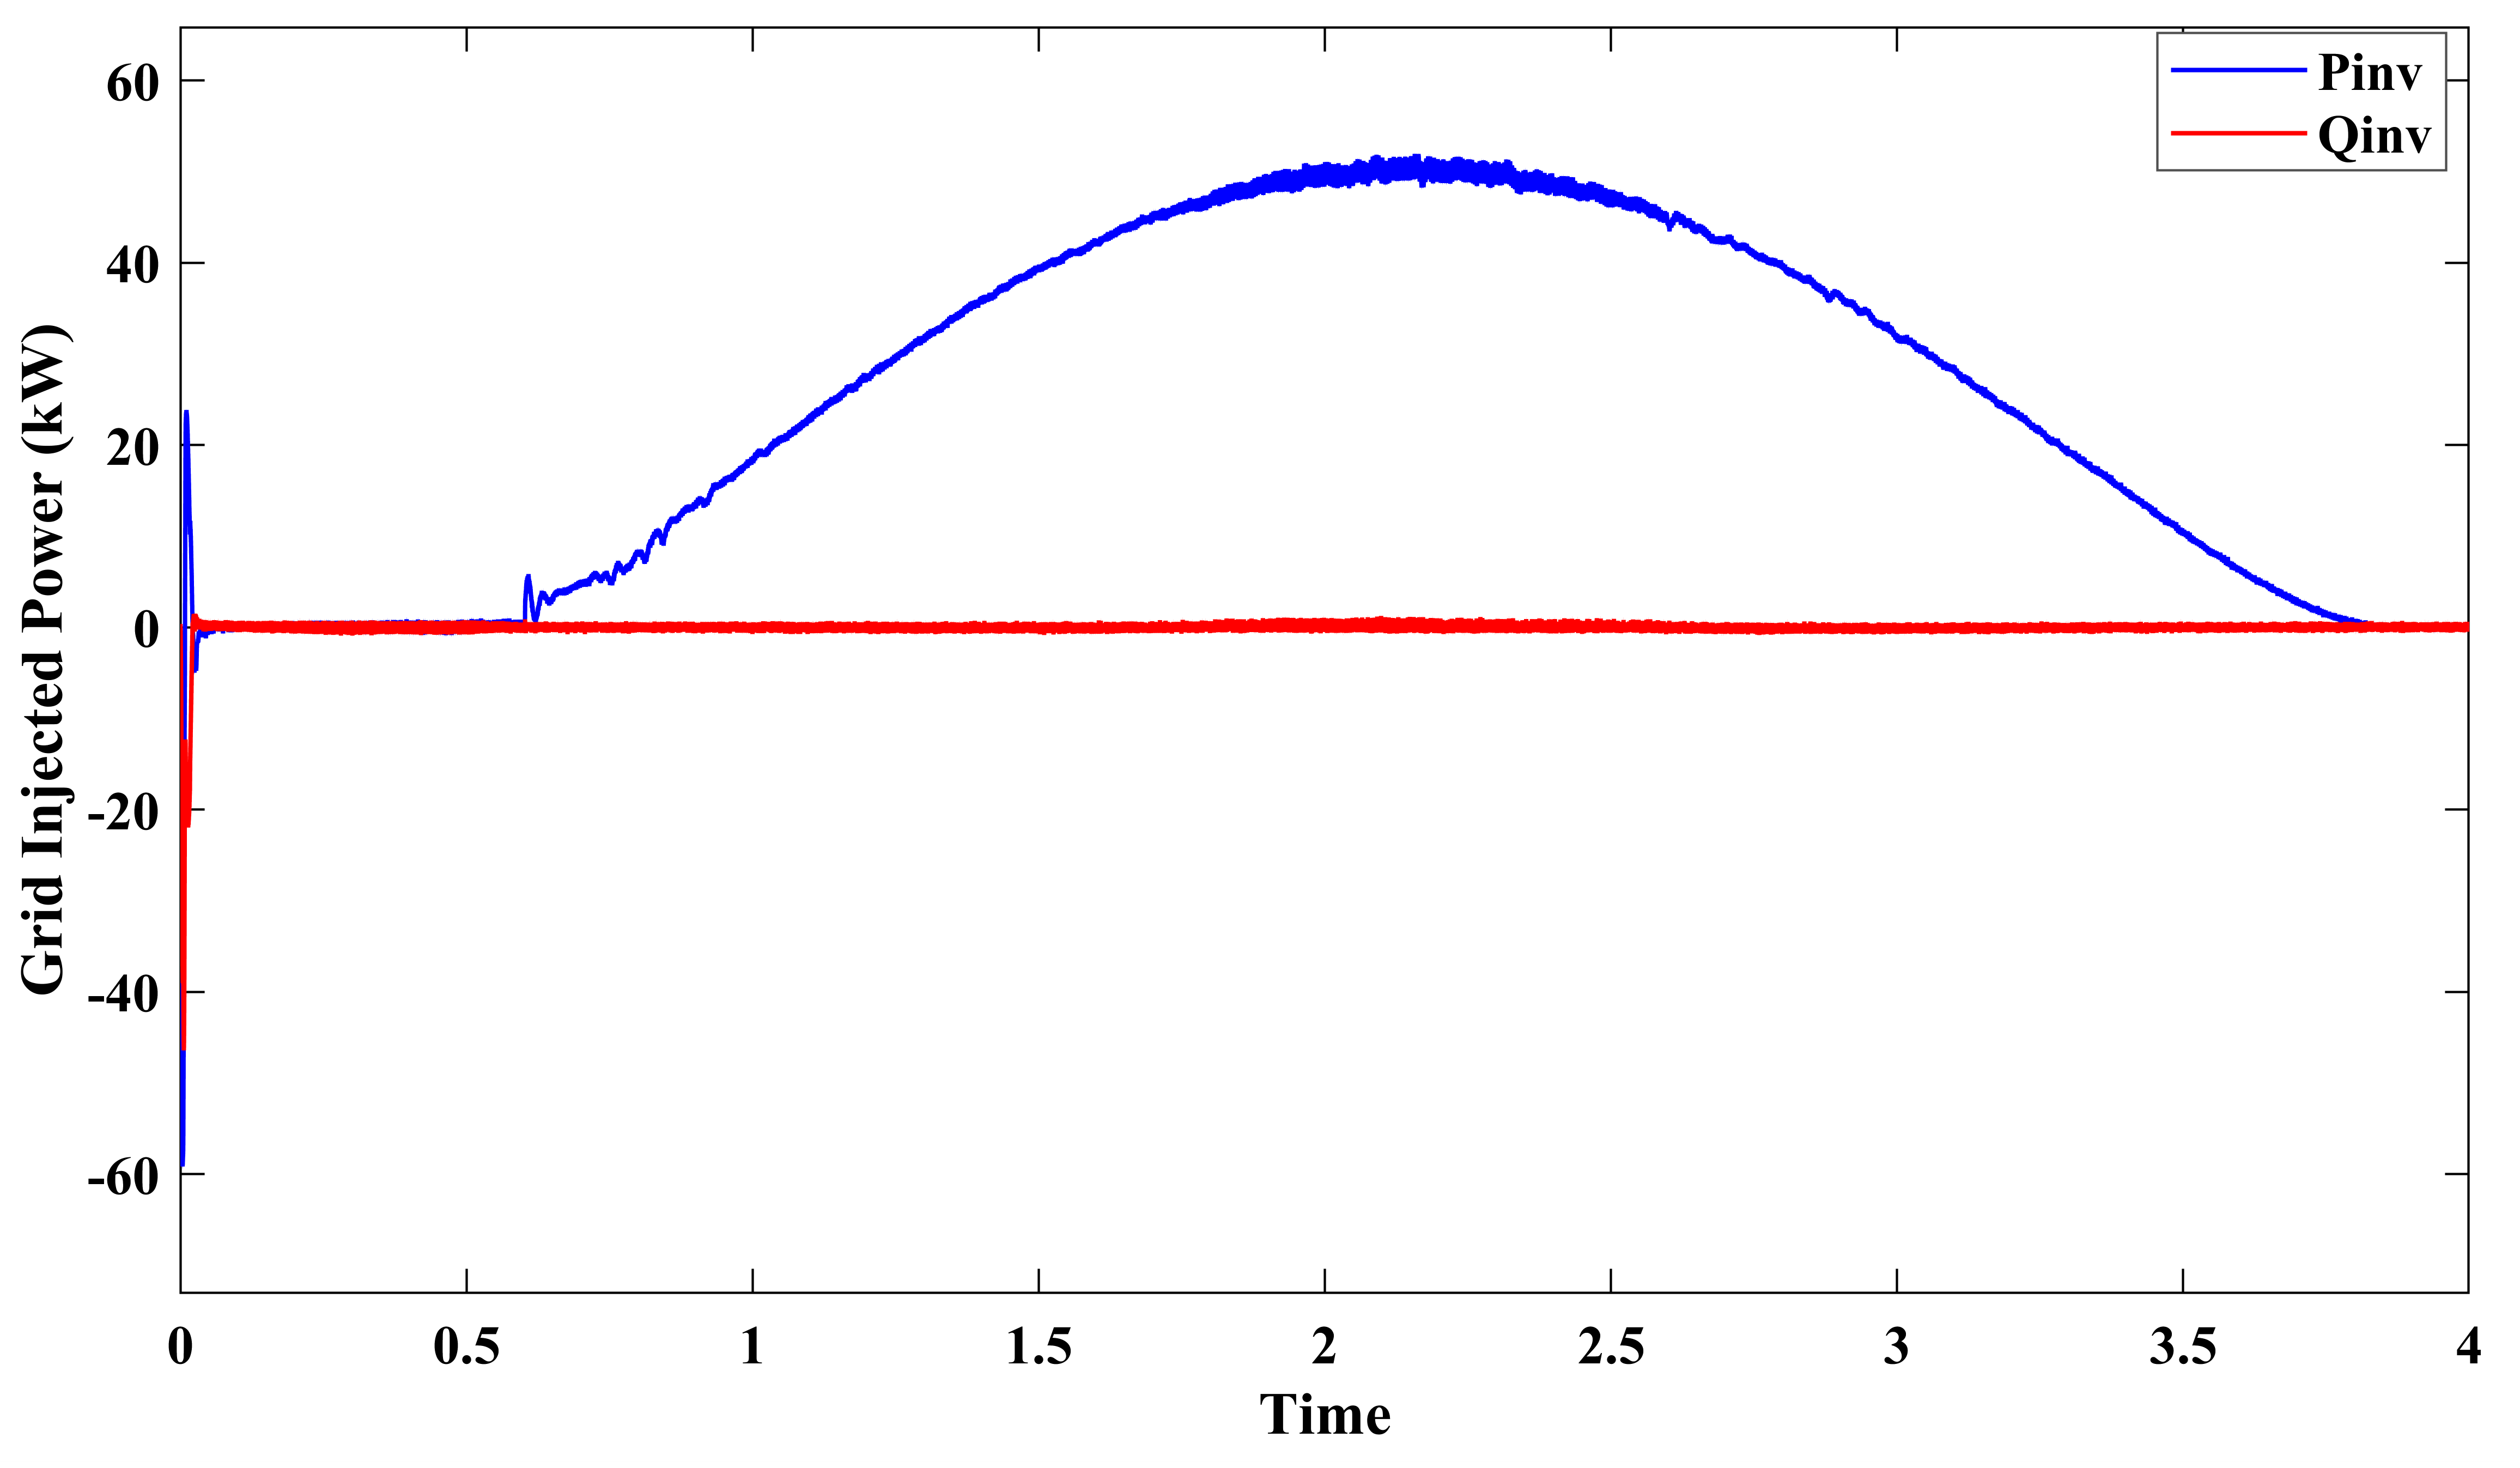
\includegraphics[width=\linewidth]{Pictures/DIC Power injected.png}
    \caption{Active power injected into the grid under DIC control}
    \label{fig:dic-grid-power}
\end{figure}

As shown in Fig.~\ref{fig:dic-grid-thd}, the grid current’s Total Harmonic Distortion (THD) is 0.84\%, significantly below the IEEE 5\% threshold. The FFT analysis confirmed the DIC’s ability to suppress high-order harmonics, thereby ensuring compliance with the grid standards.

\begin{figure}
    \centering
    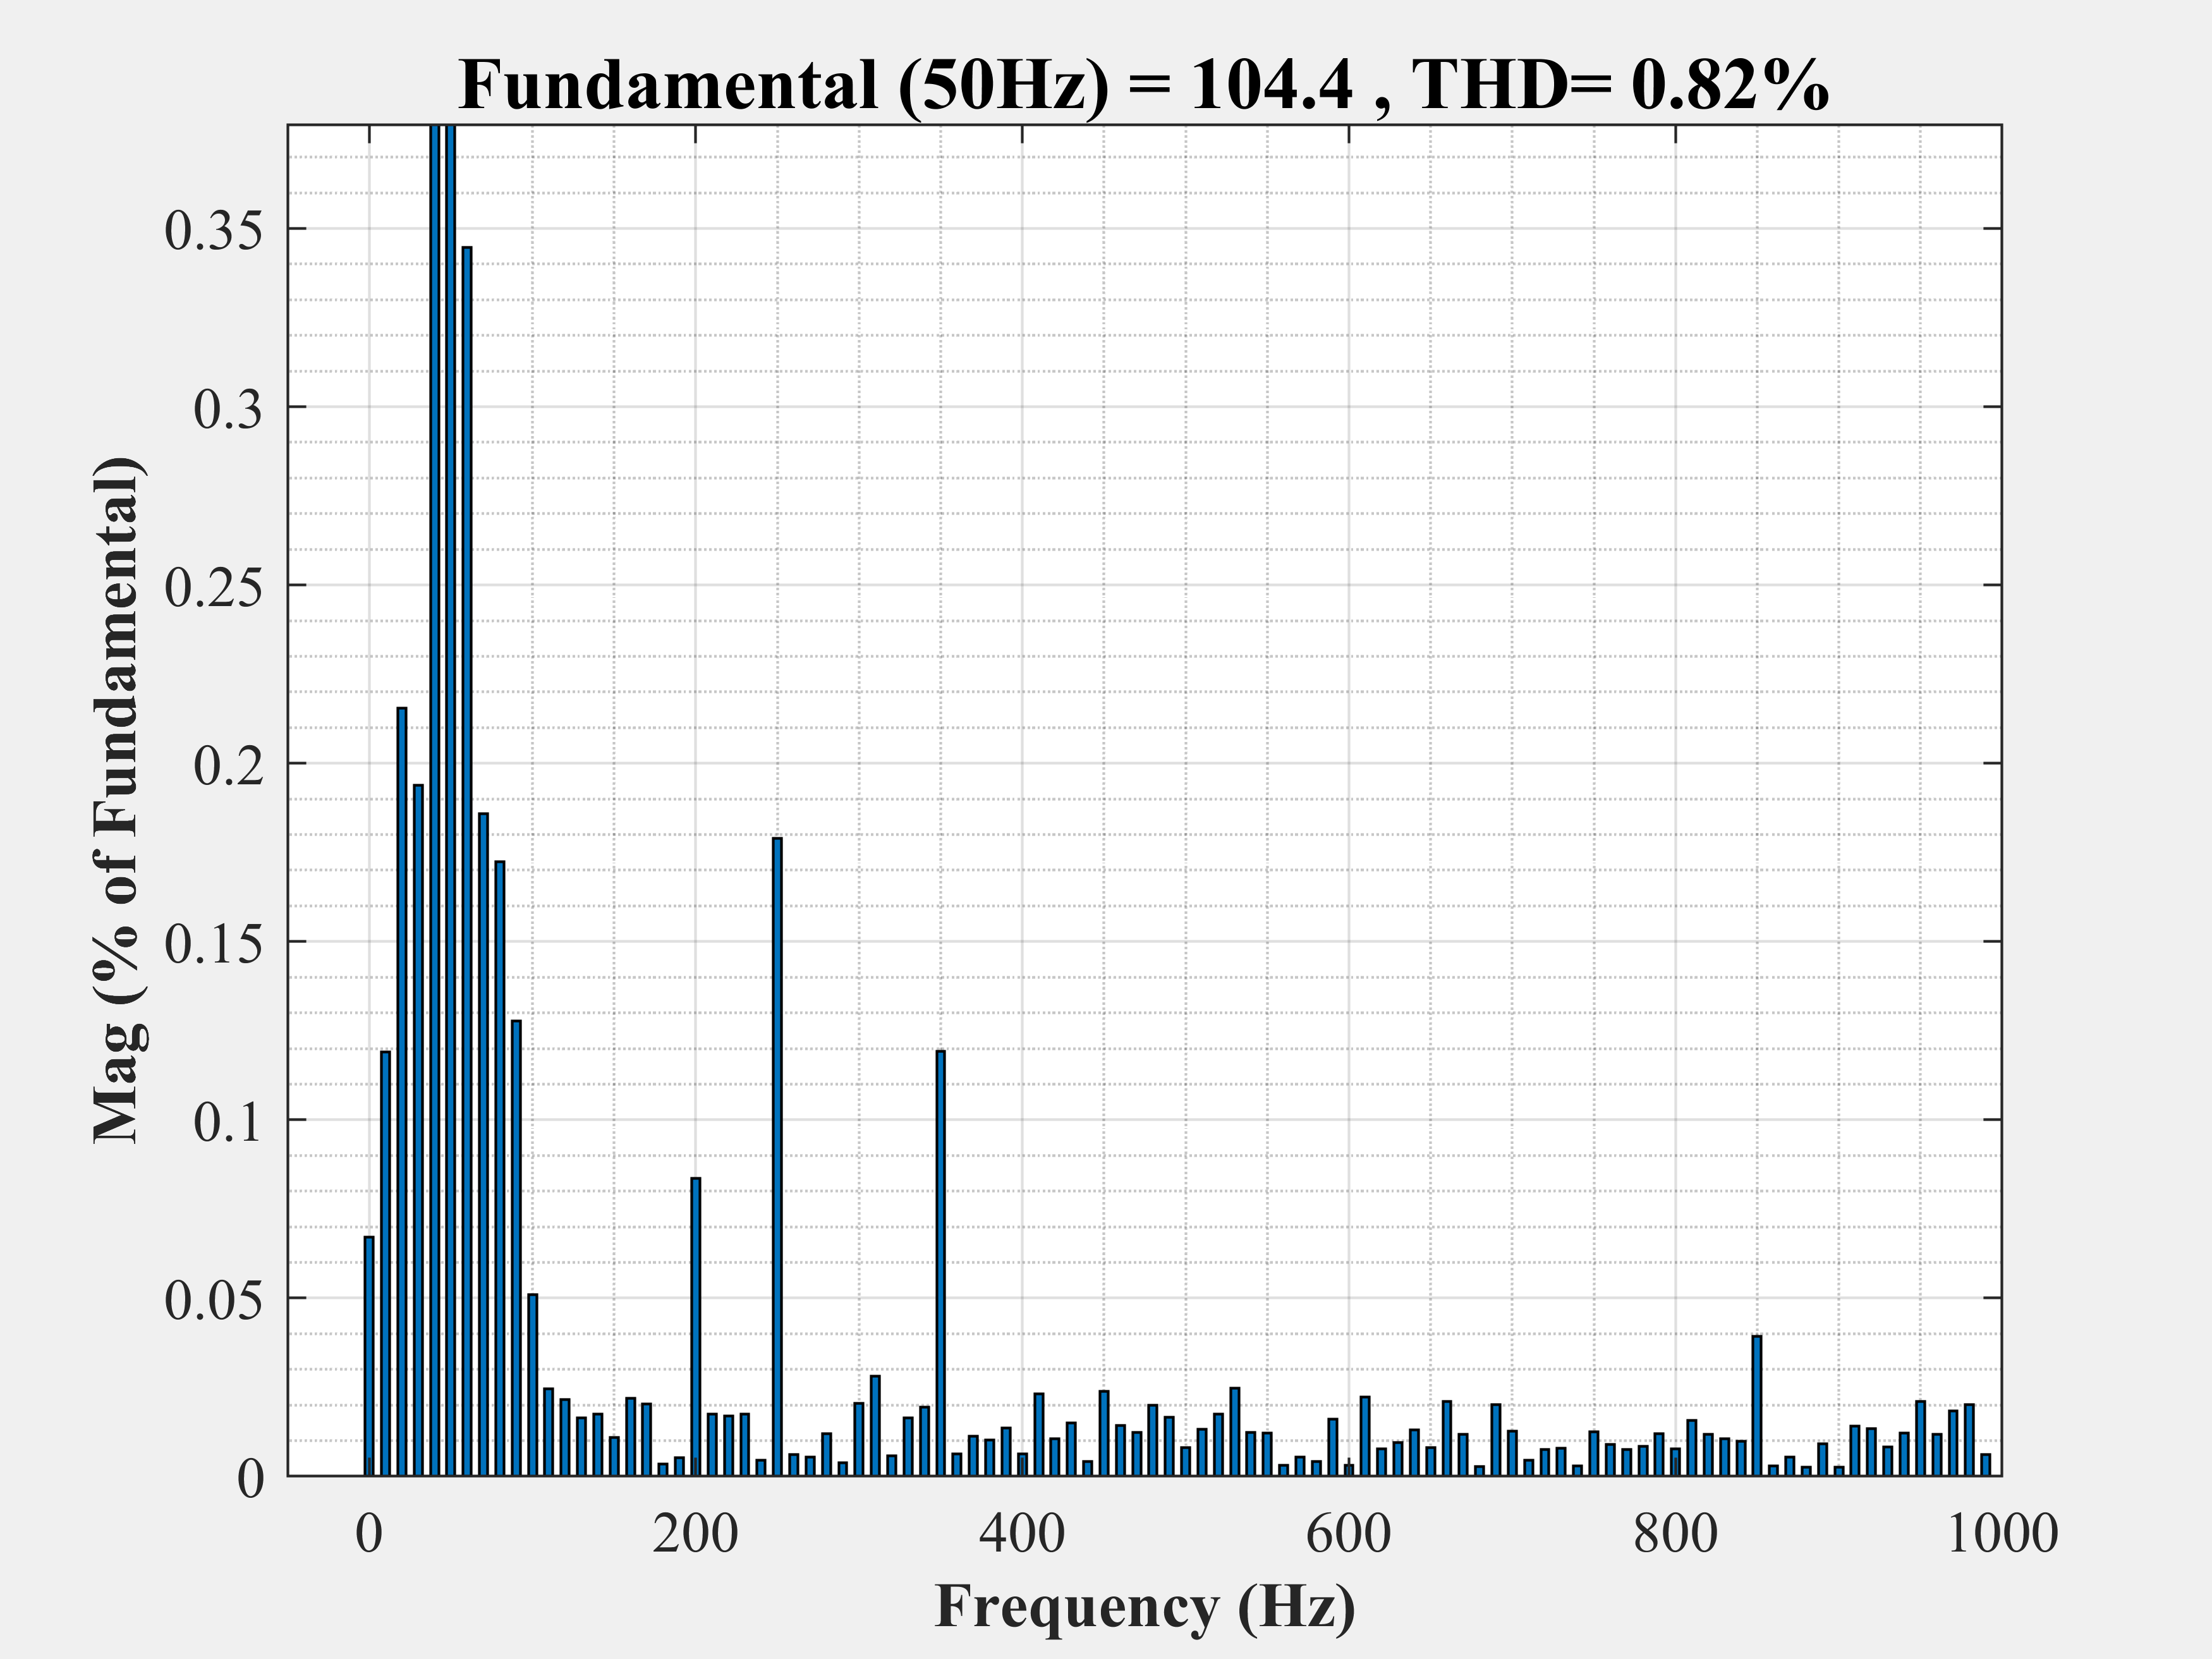
\includegraphics[width=\linewidth]{Pictures/DIC_SMC THD.png}
    \caption{Grid current THD spectrum under DIC control}
    \label{fig:dic-grid-thd}
\end{figure}

Additionally, as shown in Fig.~\ref{fig:dic-grid-synchronization}, unity power factor operation is achieved through the precise synchronization of grid voltage and current, validating the effectiveness of the controller in real-world applications.

\begin{figure}
    \centering
    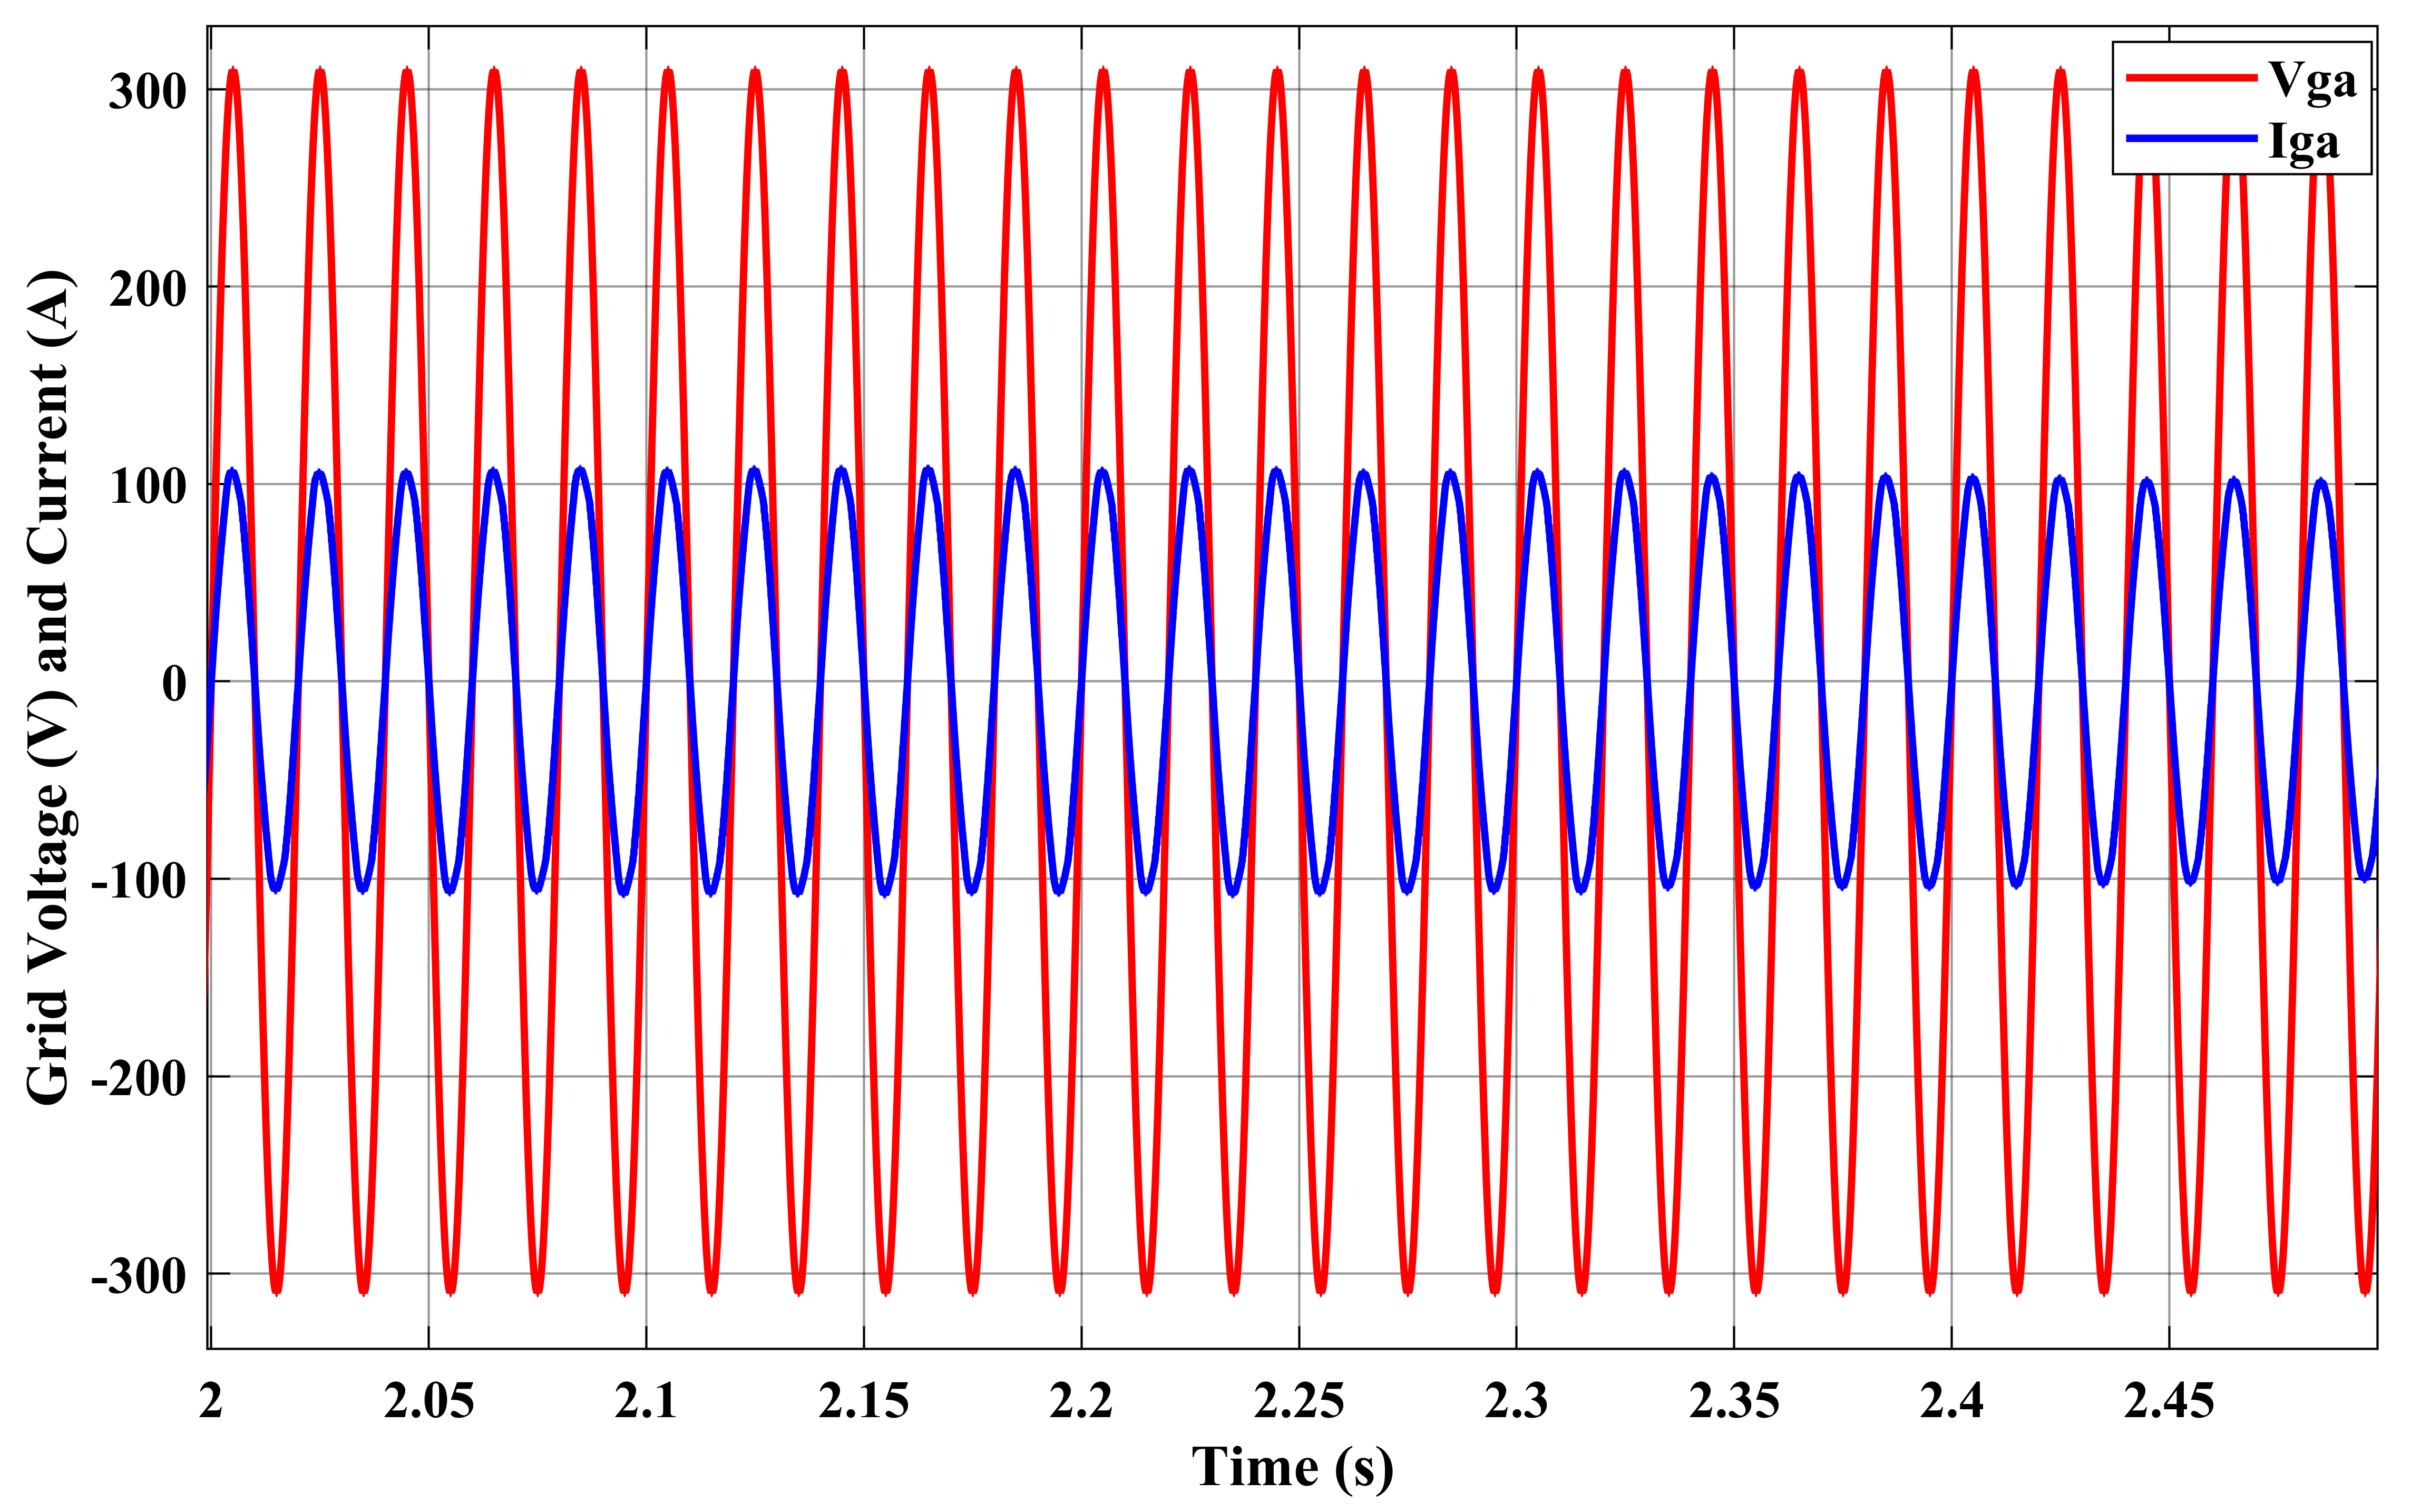
\includegraphics[width=\linewidth]{Pictures/DIC Grid voltage and current.png}
    \caption{Grid voltage-current synchronization under DIC control}
    \label{fig:dic-grid-synchronization}
\end{figure}


The gains of the proposed controllers used in the simulation are listed in Table~\ref{tab:gains}.

\begin{table}[htbp]
    \centering
    \caption{Gains of the proposed controllers used in the simulation of the model}
    \label{tab:gains}
    \begin{tabular}{c c} % Changed to 'c c' to center align data
        \toprule
        \multicolumn{2}{c}{\textbf{Continuous Twisting Algorithm Controller Gains}} \\
        \midrule
        \textbf{Parameter} & \textbf{Value} \\
        \midrule
        H  & 10 (for MPPT $\eta=1.0$) \\
        K1 & $7 \times \eta^{0.667}$ \\
        K2 & $5 \times \eta^{0.5}$ \\
        K3 & $2.3 \times \eta$ \\
        K4 & $1.1 \times \eta$ \\
        \midrule
        \multicolumn{2}{c}{\textbf{Discontinuous Integral Controller Gains}} \\
        \midrule
        \textbf{Parameter} & \textbf{Value} \\
        \midrule
        H  & 10 (for MPPT $\eta=2.0$) \\
        L  & 0.5 (for MPPT $l=30$) \\
        K1 & 1 (for MPPT $k1=0.5$) \\
        K2 & 1 (for MPPT $k2=0.05$) \\
        K3 & $\frac{\eta}{l}$ \\
        K4 & 2 (for MPPT $k4=4.5$) \\
        \bottomrule
    \end{tabular}
\end{table}

\section{Comparative Analysis}\label{sec:comparative}
The proposed Continuous Twisting Algorithm Sliding Mode Control (CTA-SMC) and Discontinuous Integral Control (DIC) were benchmarked against the conventional perturb-and-observe (P\&O)-based PI MPPT algorithm. As shown in Fig.~\ref{fig:mppt-comparison}, both CTA-SMC and DIC outperform the PI controller in terms of tracking accuracy, transient response, and power stability. The sliding mode controllers achieve smoother and faster convergence to the maximum power point (MPP) under dynamic irradiation.

\begin{equation}
\begin{aligned}
    \eta_{100}
    &= \frac{\int_{t_0}^{t_f} P_{PV} \, dt}
            {\int_{t_0}^{t_f} P_{PV\text{-}ref} \, dt} \times 100 \\
    &= \frac{\int_{t_0}^{t_f} V_{PV} I_{PV} \, dt}
            {\int_{t_0}^{t_f} P_{PV\text{-}ref} \, dt} \times 100,
       \qquad t_0=0,\quad t_f=4\,\text{s}.
\end{aligned}
\end{equation}

CTA-SMC achieved the highest efficiency (\(\eta_{100} = 99.4\%\)), followed by DIC (\(98\%\)), whereas the PI controller lagged at \(95\%\) (Fig. ~\ref{fig:dynamic-efficiency}). This underscores the superior adaptability of sliding mode controllers to transient conditions.

\begin{figure}
    \centering
    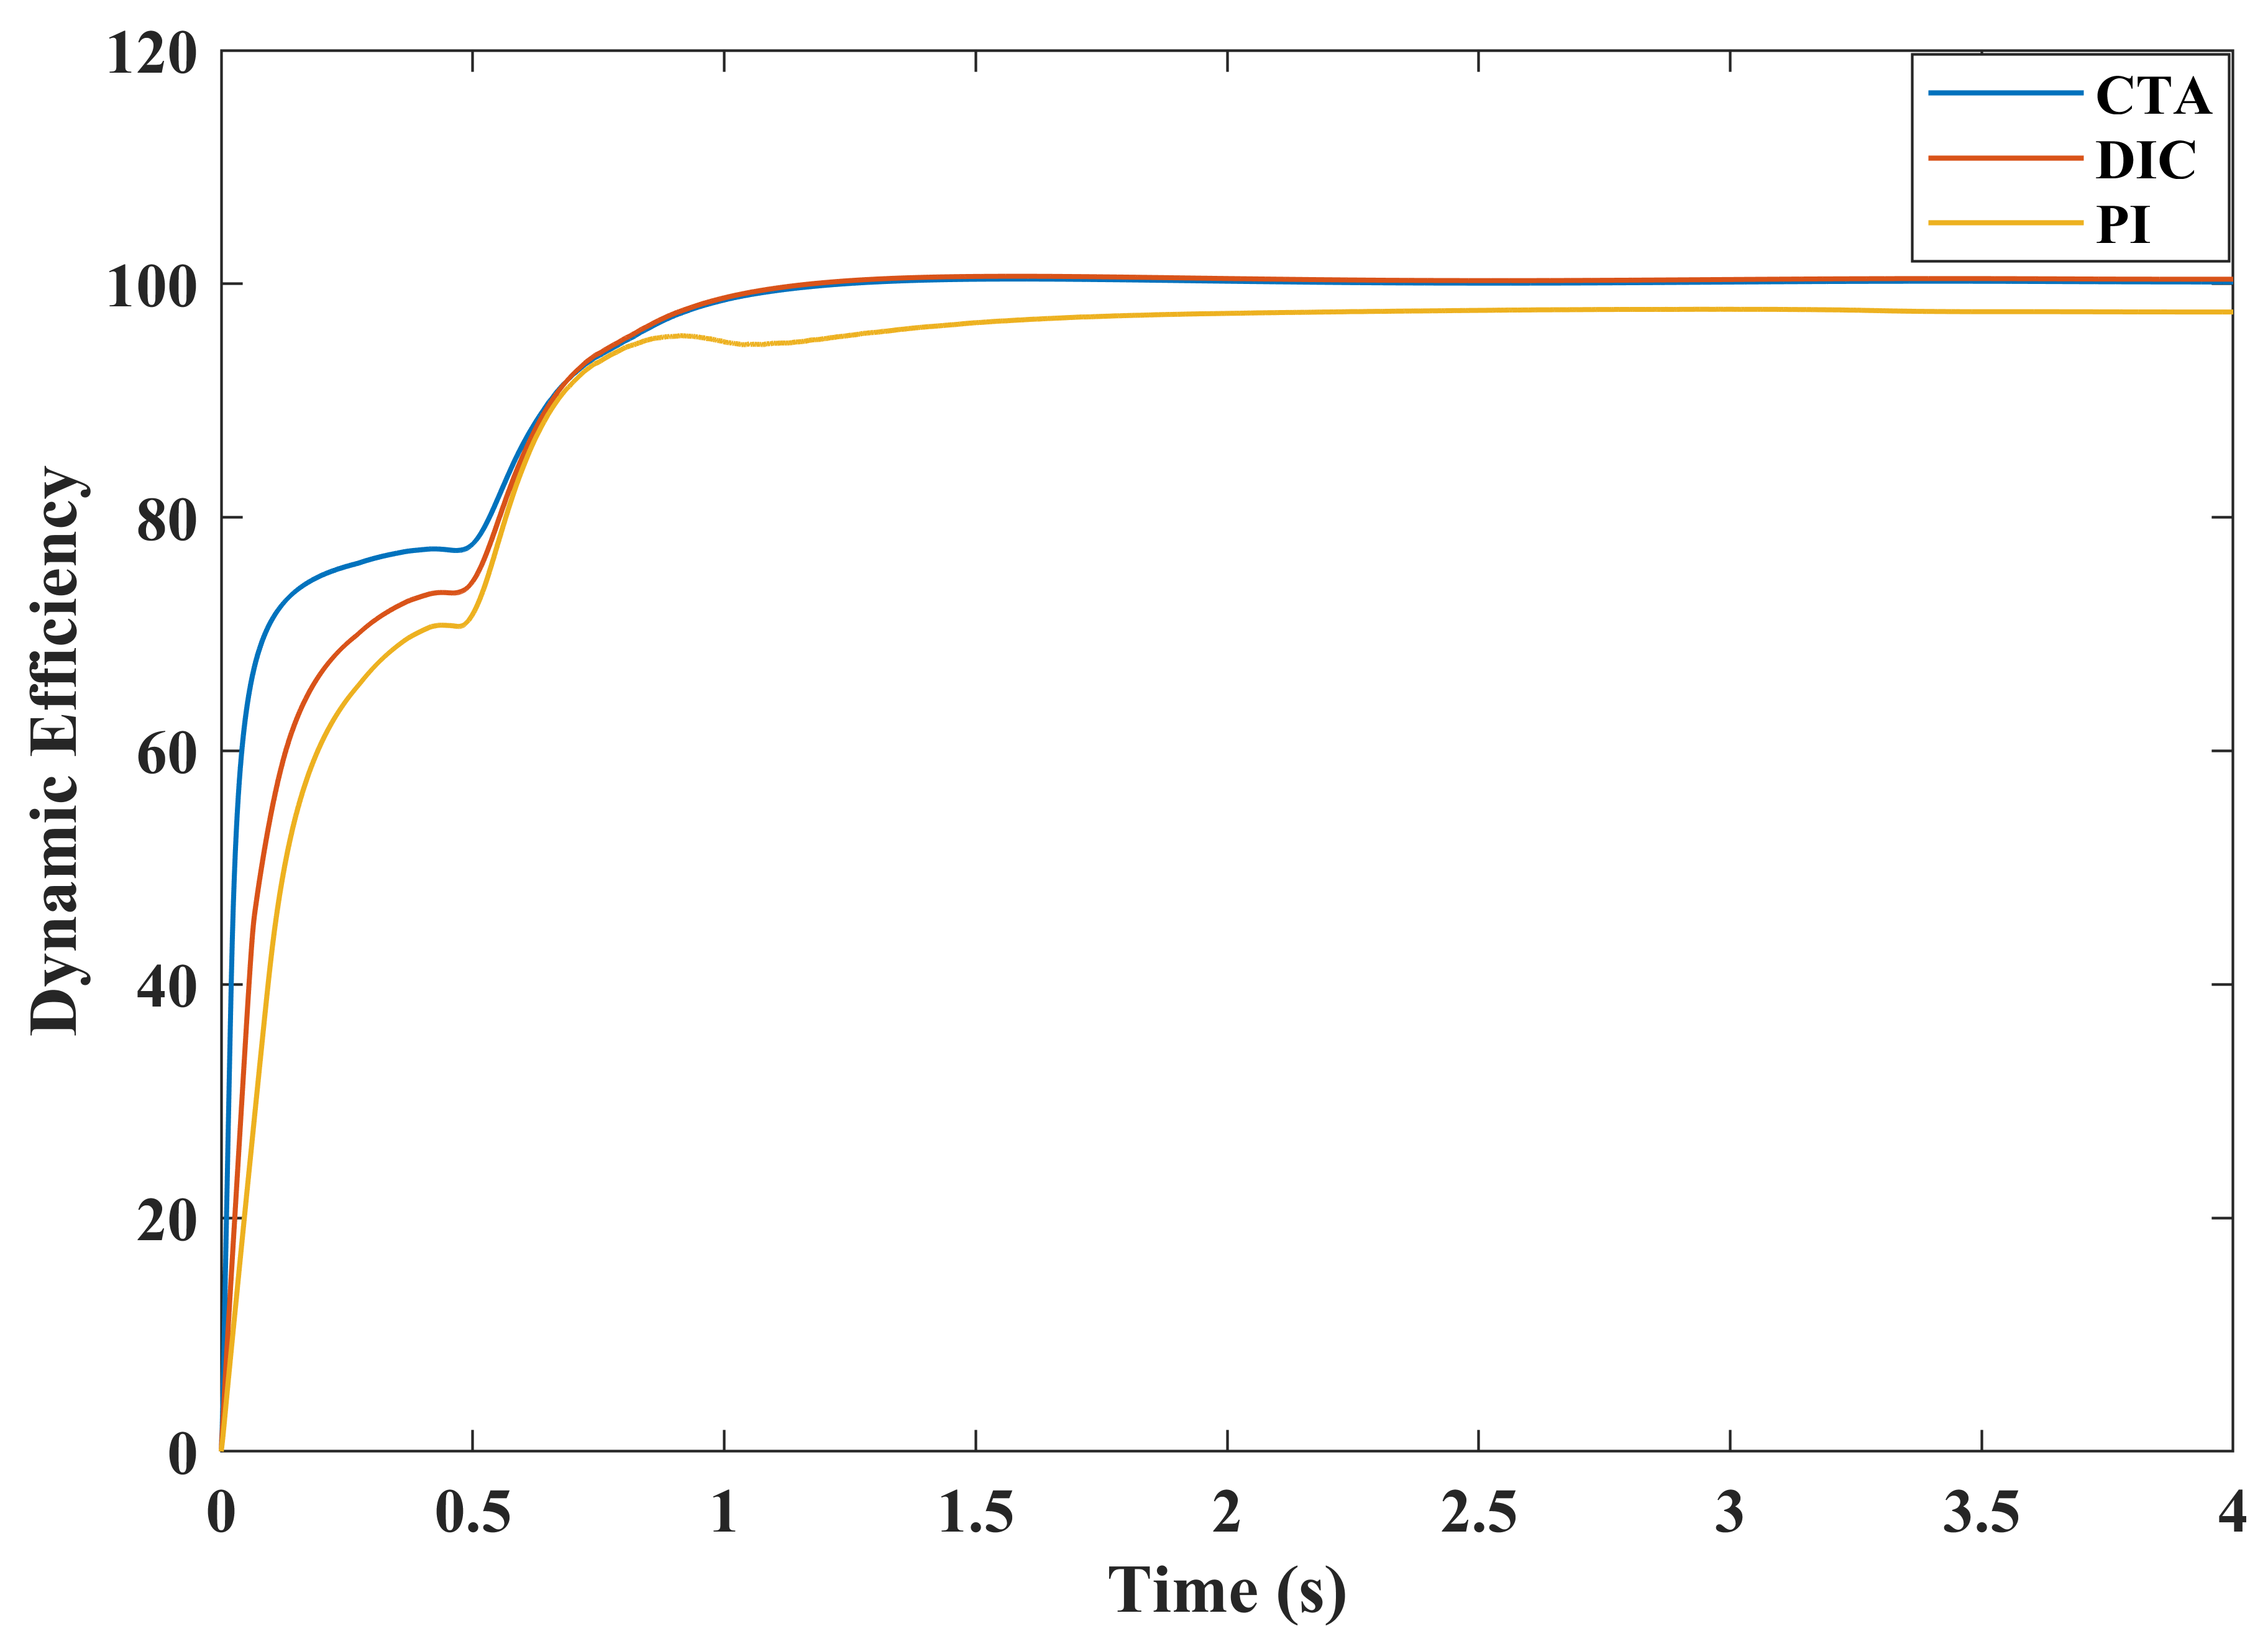
\includegraphics[width=\linewidth]{Pictures/Dynamic efficiency.png}
    \caption{Dynamic efficiency}
    \label{fig:dynamic-efficiency}
\end{figure}

The CTA-SMC delivers steady active power to the grid with minimal oscillations (Fig.~\ref{fig:grid-power-comparison}), thereby maximizing power utilization and stability. In contrast, the P\&O-PI method exhibited significant power fluctuations (``chattering''), degrading its performance. Both CTA-SMC and DIC enhance grid voltage stability and reduce Total Harmonic Distortion (THD) to \textbf{<5\%}, complying with IEEE standards (Figs. ~\ref{fig:grid-current-thd} and \ref{fig:dic-grid-thd}).
\begin{figure}
    \centering
    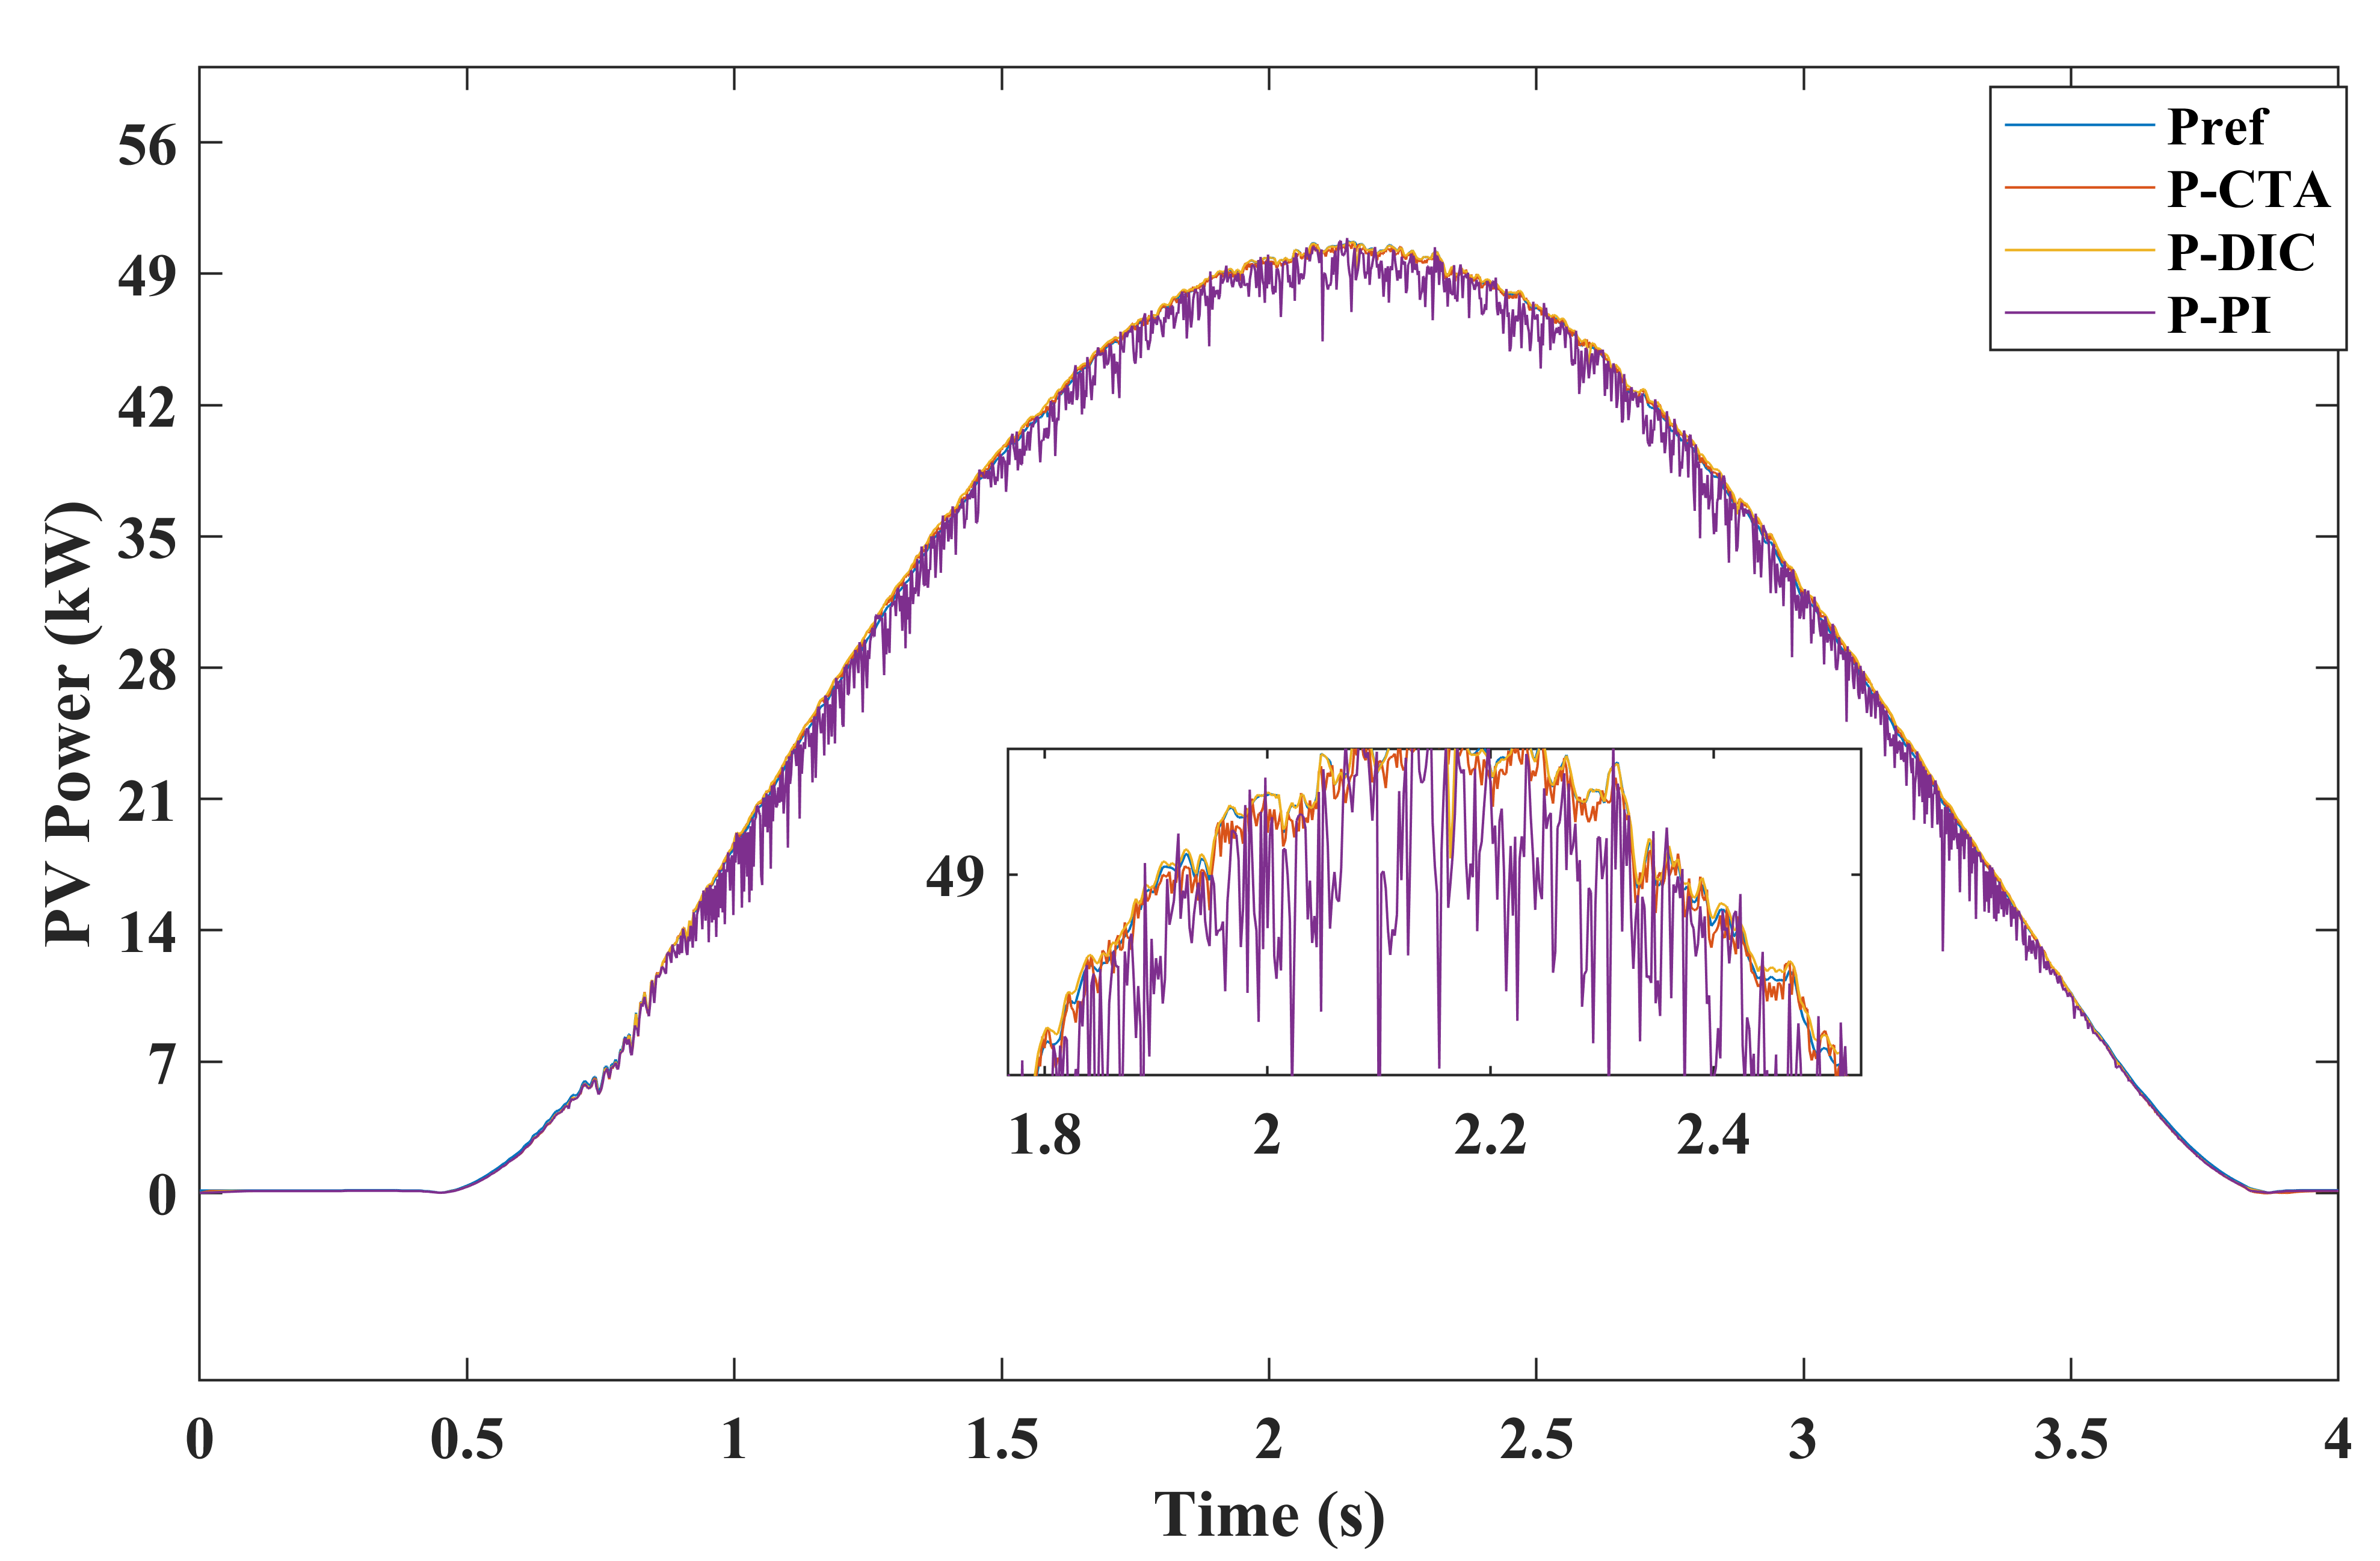
\includegraphics[width=\linewidth]{Pictures/MPPT Comparison.png}
    \caption{PV power extraction comparison}
    \label{fig:mppt-comparison}
\end{figure}
\begin{figure}
    \centering
    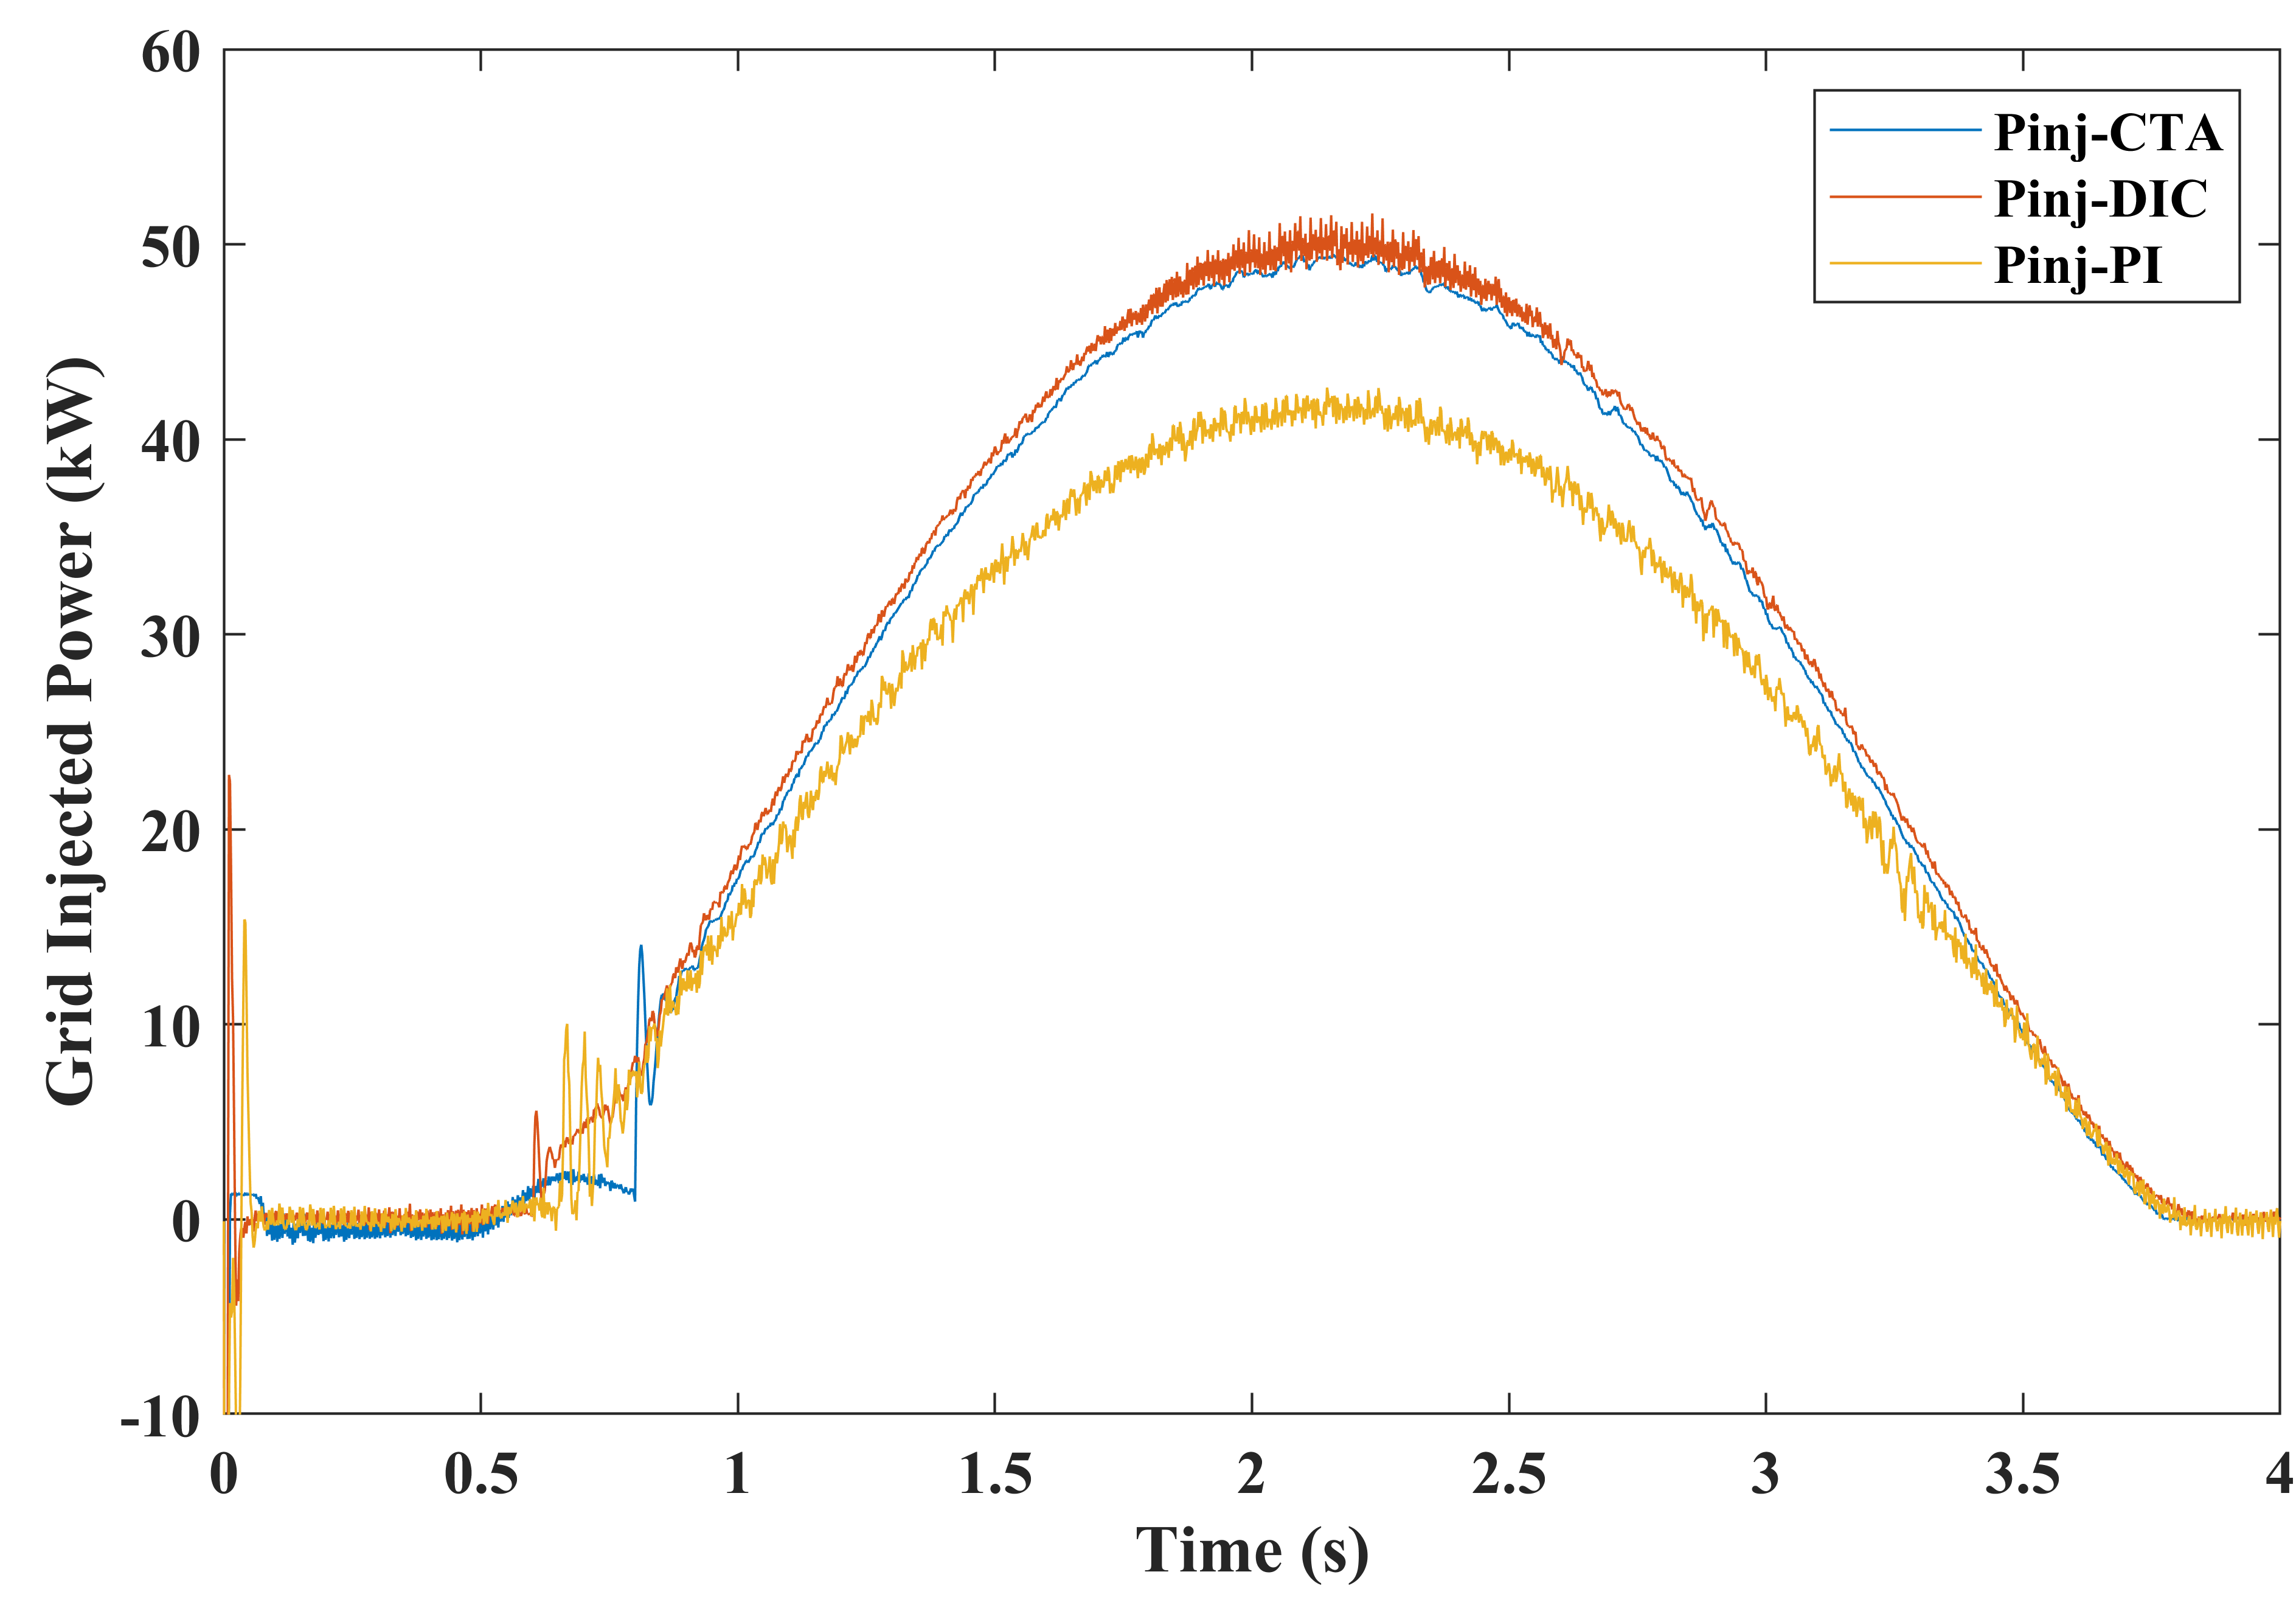
\includegraphics[width=\linewidth]{Pictures/Comparison Grid Inj Power.png}
    \caption{Grid injected power comparison }
    \label{fig:grid-power-comparison}
\end{figure}
\subsection{Performance Indices of the Employed and PI Controller}
The proposed CTA and DIC controllers were compared with the conventional PI method using four error indices: IAE, ITAE, ISE, and ITSE (Eqs. 4.1–4.4). 
\begin{equation}
    J_1 = \int_{0}^{t} |e(t)| dt \quad \text{(IAE)}
\end{equation}

\begin{equation}
    J_2 = \int_{0}^{t} t |e(t)| dt \quad \text{(ITAE)}
\end{equation}

\begin{equation}
    J_3 = \int_{0}^{t} e^2(t) dt \quad \text{(ISE)}
\end{equation}

\begin{equation}
    J_4 = \int_{0}^{t} t e^2(t) dt \quad \text{(ITSE)}
\end{equation}
These metrics were computed during the simulations (Fig. ~\ref{fig:mppt-indices} and Table~\ref{tab:mppt-indices}), reveal critical insights.
\begin{itemize}
    \item CTA achieves the lowest IAE and ITAE values, indicating minimal fluctuations and superior tracking accuracy for MPPT.
    \item DIC matches CTA in ISE and ITSE, demonstrating comparable long-term error suppression.
    \item The PI controller exhibits the highest errors across all indices, underscoring its limitations in dynamic environments.
\end{itemize}
These results emphasize the practicality of the CTA and DIC for grid-connected PV systems, in which precision and stability are paramount. Their ability to minimize errors under varying irradiance conditions ensures reliable power extraction and adherence to grid standards, outperforming conventional approaches.
\begin{figure}[htbp]
    \centering
    % First row of images
    \begin{subfigure}{0.45\textwidth}
        \centering
        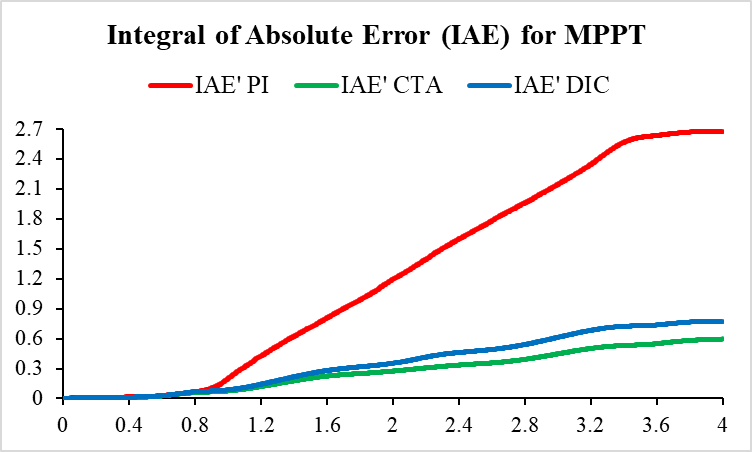
\includegraphics[width=\textwidth, height=4cm]{Pictures/IAE MPPT.png}
        \caption{IAE}
    \end{subfigure}
    \hfill
    \begin{subfigure}{0.45\textwidth}
        \centering
        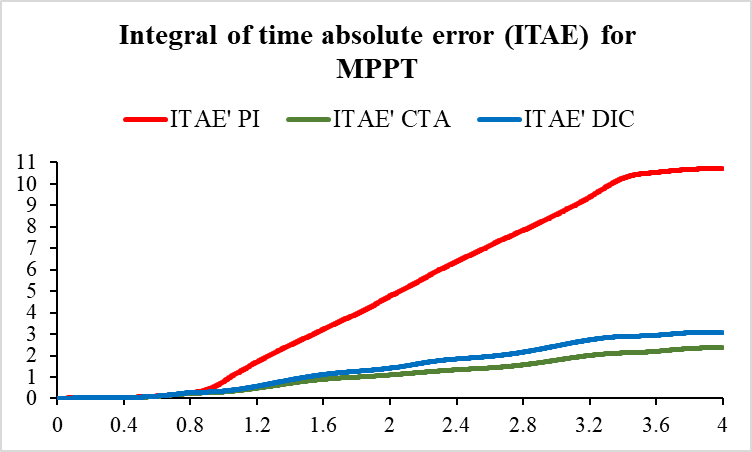
\includegraphics[width=\textwidth, height=4cm]{Pictures/ITAE MPPT.png}
        \caption{ITAE}
    \end{subfigure}

    % Second row of images
    \begin{subfigure}{0.45\textwidth}
        \centering
        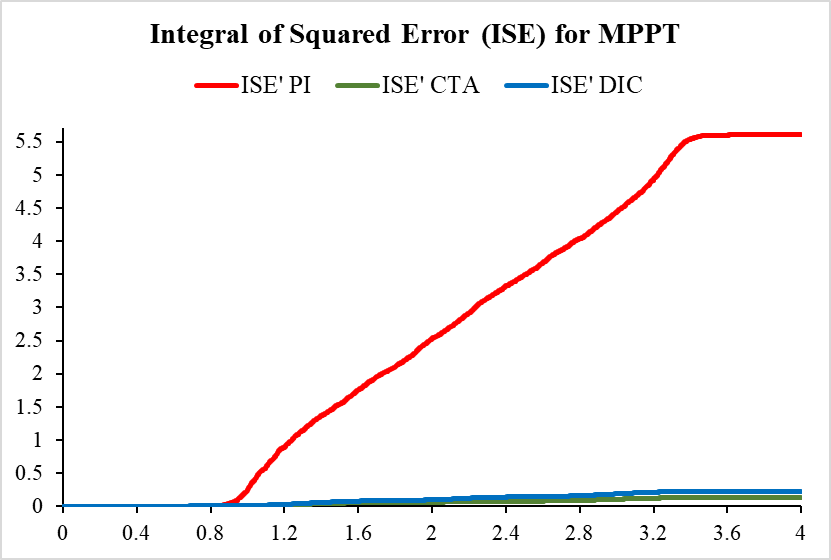
\includegraphics[width=\textwidth, height=4cm]{Pictures/ISE MPPT.png}
        \caption{ISE}
    \end{subfigure}
    \hfill
    \begin{subfigure}{0.45\textwidth}
        \centering
        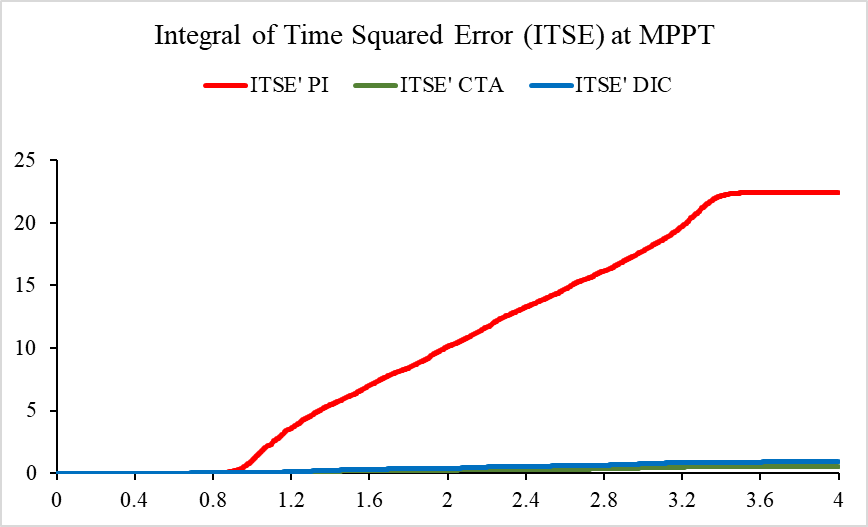
\includegraphics[width=\textwidth, height=4cm]{Pictures/ITSE MPPT.png}
        \caption{ITSE}
    \end{subfigure}

    \caption{Performance indices of the MPPT controllers PI, CTA and DIC}
    \label{fig:mppt-indices}
\end{figure}
In general, both CTA and DIC showed better performance than the PI controller, as shown in Table~\ref{tab:mppt-indices}.
\begin{table}[htbp]
    \centering
    \caption{Comparison of performance indices at MPPT Controller}
    \label{tab:mppt-indices}
    \renewcommand{\arraystretch}{1.3} % Better row spacing
    
    % Scale table to textwidth
    \resizebox{\textwidth}{!}{%
    \begin{tabular}{l c c c c c}
        \hline
        \multicolumn{6}{c}{\textbf{Performance Indices Comparison in tabulated form for MPPT/DC-DC Boost Controller}} \\
        \hline
        \textbf{Control Strategy} & \textbf{Efficiency} & \textbf{IAE} & \textbf{ITAE} & \textbf{ISE} & \textbf{ITSE} \\
        \hline
        CTA-SMC  & 99.4\%  & 0.5750  & 2.2998  & 0.1375  & 0.5501  \\
        DIC-SMC  & 98\%    & 0.7596  & 3.0386  & 0.2283  & 0.9133  \\
        PI       & 95\%    & 2.6615  & 10.6461 & 5.6062  & 22.4250 \\
        \hline
    \end{tabular}%
    }
\end{table}

The Total Harmonic Distortion (THD) of the grid current was analyzed for the proposed CTA and DIC controllers alongside the conventional PI method (Fig. ~\ref{fig:inverter-indices} and Table~\ref{tab:inverter-indices}). Key findings include:
\begin{itemize}
 \item CTA Controller: Achieves the lowest THD $\leq 0.5\%$, outperforming both DIC and PI in minimizing harmonic distortion. Its superior error indices (IAE, ITAE, ISE, and ITSE) reflect precise harmonic suppression with minimal transient fluctuations.

\item DIC Controller: Exhibits marginally higher THD $(\leq 0.8\%)$ but demonstrates exceptional stability with the smallest accumulated error over time (ITSE), ensuring robust operation under prolonged grid disturbances.

\item PI Controller: Records the highest THD and error indices, highlighting its inadequacy in harmonic mitigation.
\end{itemize}
These results validate the CTA as the optimal choice for THD-sensitive applications, whereas the DIC excels in scenarios prioritizing long-term stability. Both controllers comply with the IEEE 519 standard $(THD \leq 5\%)$, ensuring grid compatibility and enhanced power quality.

\begin{figure}[htbp]
    \centering
    % First row of images
    \begin{subfigure}{0.45\textwidth}
        \centering
        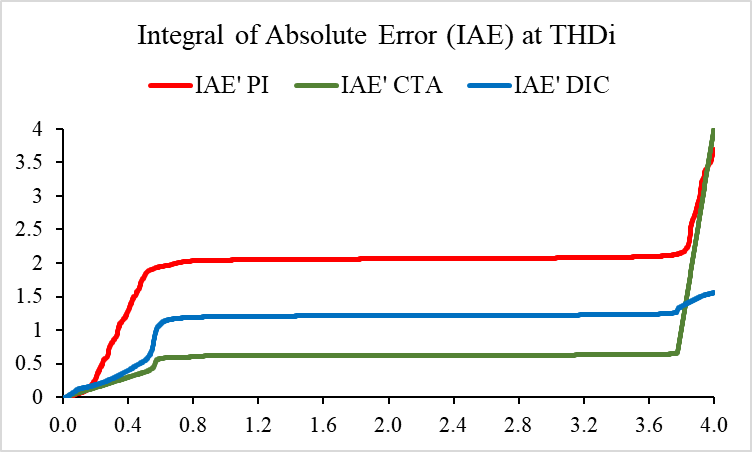
\includegraphics[width=\textwidth, height=4cm]{Pictures/IAE INVER.png}
        \caption{IAE}
    \end{subfigure}
    \hfill
    \begin{subfigure}{0.45\textwidth}
        \centering
        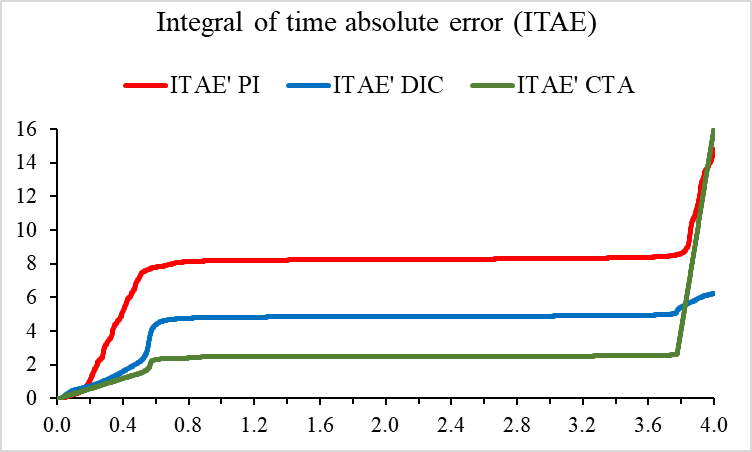
\includegraphics[width=\textwidth, height=4cm]{Pictures/ITAE INVER.png}
        \caption{ITAE}
    \end{subfigure}

    % Second row of images
    \begin{subfigure}{0.45\textwidth}
        \centering
        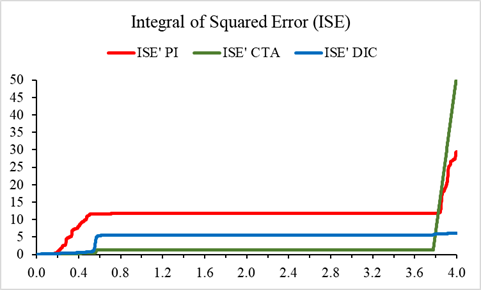
\includegraphics[width=\textwidth, height=4cm]{Pictures/ISE INVER.png}
        \caption{ISE}
    \end{subfigure}
    \hfill
    \begin{subfigure}{0.45\textwidth}
        \centering
        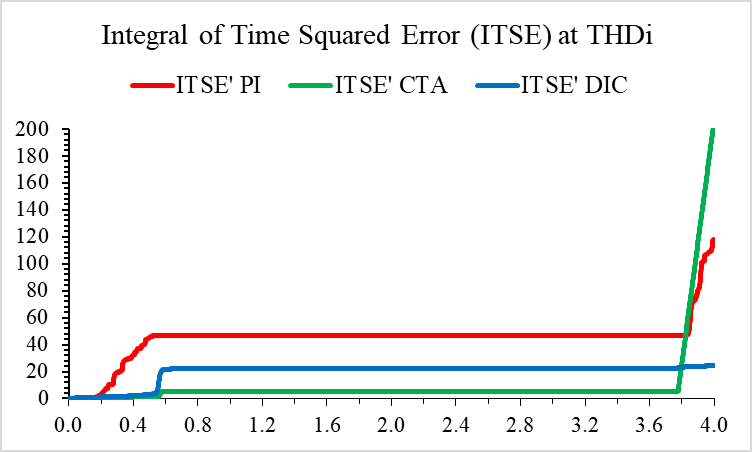
\includegraphics[width=\textwidth, height=4cm]{Pictures/ITSE INVER.png}
        \caption{ITSE}
    \end{subfigure}
    
    \caption{Performance indices of the Inverter Controllers PI, CTA and DIC}
    \label{fig:inverter-indices}
\end{figure}
\begin{table}[htbp]
    \centering
    \caption{Comparison of performance indices for inverter control}
    \label{tab:inverter-indices}
    \renewcommand{\arraystretch}{1.2}
    % Resize to fit page width
    \resizebox{\textwidth}{!}{%
    \begin{tabular}{lccccc}
        \toprule
        \multicolumn{6}{c}{\textbf{Comparison of Performance Indices for Inverter Controller}} \\
        \midrule
        \textbf{Control Strategy} & \textbf{THD} & \textbf{IAE} & \textbf{ITAE} & \textbf{ISE} & \textbf{ITSE} \\
        \midrule
        CTA-SMC & 0.43\% & 0.6458 & 2.5917 & 1.3167 & 5.2668 \\
        DIC-SMC & 0.82\% & 1.2528 & 5.0262 & 5.4907 & 21.9627 \\
        PI      & 2.27\% & 2.1180 & 8.4850 & 11.7053 & 46.8213 \\
        \bottomrule
    \end{tabular}%
    }
\end{table}


%\section{Summary}
The proposed design was tested under varying solar irradiances and showed remarkable improvement. The observer results were simulated using the two control techniques. The observer efficiently estimated the system states for both proposed control techniques. With the help of two states, all six states (inverter output current d component, inverter output q component, voltage across capacitor d component, voltage across q component, grid current d component, and grid current q component) of the system were calculated. These estimated states were used in place of the actual states, which were the three-phase grid current, grid voltage, and capacitor voltage. The proposed controllers maintained exact tracking under various solar irradiation conditions compared with the PI controller. In addition, the proposed controllers enhance the quality of the output power by reducing THD. The use of the LCL filter allows us to use small values for the inductor and capacitor.
\section{Conclusion}
\label{sec:conclusion}
This study demonstrates the successful implementation of the Continuous Twisting Algorithm (CTA) and Discontinuous Integral Controller (DIC) sliding mode controls in a two-stage grid-connected PV system. Both controllers outperform conventional PI methods, with the CTA and DIC achieving rapid maximum power point tracking (MPPT) under dynamic irradiance by dynamically adjusting the PV reference voltage \(V_{ref}\) derived from the perturb-and-observe (P\&O) method. For grid integration, the controllers regulate the inverter via \(i^*_{gd}\) (linked to the DC-link voltage) and enforce \(i^*_{gq}=0\) to ensure a unity power factor and minimal reactive power injection. An LCL filter minimizes the THD to $\leq 5\%$, complying with the IEEE standards, whereas a Utkin sliding mode observer enhances the accuracy by estimating the inverter current and capacitor voltage in the dq-frame. The finite-time convergence and robustness properties of the CTA and DIC used in this study follow from the sliding-mode control results established in \cite{torres2017design, moreno2017discontinuous}. In the reported simulations, the CTA excelled in harmonic suppression ($THD \leq 0.5\%$), whereas the DIC prioritized steady-state precision by minimizing cumulative errors. These results underscore the practical value of sliding mode strategies in balancing the efficiency, stability, and grid compliance of renewable energy systems.

\subsection*{Limitations and Future Work}
The present study is based entirely on MATLAB/Simulink simulations, and the reported performance metrics correspond to an idealized modeling environment. Consequently, several practical aspects are outside the scope of this study. First, the real-time computational costs of the CTA and DIC have not been characterized, and their behavior on embedded controllers with finite sampling rates, quantization, and measurement noise remains to be assessed. Second, no hardware-in-the-loop (HIL) or experimental validation on a physical PV/inverter setup has been conducted; such validation is required to confirm that the observer-based, sensor-reduced implementation performs as predicted under real grid disturbances, partial shading, and component tolerances. Third, the study assumes a balanced and healthy grid and does not explicitly address abnormal conditions, such as grid voltage sags, faults, or islanding events. Therefore, future work will focus on (i) real-time and HIL implementation of the CTA/DIC-based controllers together with the Utkin observer, (ii) extending the framework to fault-tolerant operation and unbalanced grid conditions, and (iii) rigorous quantification of computational complexity and tuning sensitivity for deployment on typical embedded control platforms.
% \section{Future Work}
% \label{sec}
 %The following are useful future research potentialities of this model, which are more realistic in nature.
%\begin{itemize}
 

%\item \textbf{AI-Driven MPPT Tracking}: Integrate machine/deep learning techniques for predictive MPPT control, enhancing adaptability to nonlinear PV behaviors and real-time efficiency.
    
 %   \item \textbf{Hybrid Voltage Control}: Combine model predictive control (MPC) with robust strategies to stabilize DC-link voltage rapidly, minimizing overshoots and ensuring grid continuity.
    
  %  \item \textbf{Advanced Harmonic Mitigation}: Develop adaptive resonant controllers or dynamic compensators to suppress harmonics during non-power transfer and transient conditions.
    
   % \item \textbf{Hybrid Control Schemes}: Merge continuous/discontinuous methods to improve grid synchronization and reduce oscillations during PV generation fluctuations.
    
    %\item \textbf{Fault-Resilient Controllers}: Embed fault detection and self-correction mechanisms to address partial shading, voltage sags, and component failures.
    
    %\item \textbf{Predictive Fault Management}: Design controllers with preemptive diagnostic algorithms to anticipate and mitigate system failures, boosting reliability.
%\end{itemize}
%% Use \subsubsection, \paragraph, \subparagraph commands to 
%% start 3rd, 4th and 5th level sections.
%% Refer following link for more details.
%% https://en.wikibooks.org/wiki/LaTeX/Document_Structure#Sectioning_commands



%% Refer following link for more details.
%% https://en.wikibooks.org/wiki/LaTeX/Mathematics
%% https://en.wikibooks.org/wiki/LaTeX/Advanced_Mathematics

%% Use a table environment to create tables.
%% Refer following link for more details.



%% Use figure environment to create figures
%% Refer following link for more details.
%% https://en.wikibooks.org/wiki/LaTeX/Floats,_Figures_and_Captions



%% The Appendices part is started with the command \appendix;
%% appendix sections are then done as normal sections
%\appendix
%\section{Example Appendix Section}
%\label{app1}

%Appendix text.

%% For citations use: 
%%       \cite{<label>} ==> [1]

%%
%Example citation, See \cite{lamport94}.

%% If you have bib database file and want bibtex to generate the
%% bibitems, please use
%%
\newpage
\bibliographystyle{elsarticle-num} 
\bibliography{references-reviewed}

%% else use the following coding to input the bibitems directly in the
%% TeX file.

%% Refer following link for more details about bibliography and citations.
%% https://en.wikibooks.org/wiki/LaTeX/Bibliography_Management

%\begin{thebibliography}{00}

%% For numbered reference style
%% \bibitem{label}
%% Text of bibliographic item

%\bibitem{lamport94}
 % Leslie Lamport,
 % \textit{\LaTeX: a document preparation system},
  %Addison Wesley, Massachusetts,
  %2nd edition,
  %1994.

%\end{thebibliography}
\end{document}

\endinput
%%
%% End of file `elsarticle-template-num.tex'.
